\documentclass[../main.tex]{subfiles}
\graphicspath{{\subfix{../images/}}}

\begin{document}

\chapter{Электричество и магнетизм}

\section{Электрическое поле в вакууме}
Наименьший заряд в природе обозначается как \texttt{e} и называется электроном. Из такого утверждения, следует что любой заряд в природе может быть определён как  $ q = \pm e \cdot N, N \in \mathbb{Z}$

\vspace{5px}

Заряд --- величина дискретная, может быть положительной и отрицательной, при соприкосновении разноименных зарядов они взаимоуничтожаются.
\subsection{Закон сохранения заряда}
\textit{\textbf{Формулировка:} Заряд сохраняется в электрически замкнутой системе.}

\define Электрически замкнутая система - система, через границу которой не проходят электрические заряды.

\subsection{Закон Кулона}
\textit{\textbf{Формулировка:} Все заряженные тела взаимодействуют между собой. При этом одноименные заряды отталкиваются, а разноименные притягиваются.}
Причем сила с которой они взаимодействуют равна:
\[ F = k\frac{q_1 q_2}{r^2}\]
\begin{center}
    где k - коэффициент пропорциональности,  $q_1,q_2$ - величины зарядов
\end{center}

\define \textbf{Точечным зарядом} называется заряженное тело, размером которого можно пренебречь по сравнению с расстоянием до других заряженных тел.

\vspace{5px}

В системе СИ заряд измеряют в Кулонах, при этом Кулон не основная единица измерения, а составная: $[q] = \text{Кл} = \text{Ам} \cdot \text{c}$.
При измерении в Кулонах коэффициент k будет равен $k = 9 \cdot 10^9 \frac{\text{Н} \cdot \text{м}^2}{\text{Кл}^2}$

На практике в опытах также возникал некоторый коэффициент, поэтому при решении задач используют уже нормализованную форму:
\[ k = \frac{1}{4 \pi \varepsilon_0}\]
\begin{center}
    где $\varepsilon_0$ электрическая постоянная, $\varepsilon_0 = 8,85 \cdot10^{-12} \frac{\text{Ф}}{\text{м}}$
\end{center}

\[F = \frac{1}{4 \pi \varepsilon_0}\frac{q_1 q_2}{r^2}\]

\section{Электрическое поле}
\define Напряженность электрического поля
\[ \vec E = \frac{\vec F}{q} \text{(векторная)}\]
\begin{center}
    \definecolor{qqqqff}{rgb}{0,0,1}
    \definecolor{ffqqqq}{rgb}{1,0,0}
    \begin{tikzpicture}[line cap=round,line join=round,>=triangle 45,x=1.5755455765500463cm,y=1.4141895319101883cm]
        \clip(26.95,39.98) rectangle (37.37,42.39);
        \draw [line width=1.6pt,color=ffqqqq] (33,41) ellipse (0.45cm and 0.4cm);
        \draw [color=ffqqqq](32.83,41.34) node[anchor=north west] {$+$};
        \draw [line width=1.6pt,color=qqqqff] (35,41) ellipse (0.45cm and 0.4cm);
        \draw [color=qqqqff](34.82,41.34) node[anchor=north west] {$-$};
        \draw [->] (35.28,40.99) -- (36.4,40.97);
        \draw (35.57,41.77) node[anchor=north west] {$\vec E$};
        \draw [->] (34.71,40.99) -- (33.69,40.97);
        \draw (34.19,41.75) node[anchor=north west] {$\vec F$};
        \draw [line width=1.6pt,color=ffqqqq] (29.17,45.85) ellipse (0.45cm and 0.4cm);
        \draw [color=ffqqqq](29,46.2) node[anchor=north west] {$+$};
        \draw [line width=1.6pt,color=qqqqff] (31.87,45.96) ellipse (0.45cm and 0.4cm);
        \draw [color=qqqqff](31.75,46.34) node[anchor=north west] {$-$};
        \draw (32.91,41.74) node[anchor=north west] {q};
        \draw (34.82,41.94) node[anchor=north west] {$q_{\text{пр}}$};
        \draw [line width=1.6pt,color=ffqqqq] (27.96,41) ellipse (0.45cm and 0.4cm);
        \draw [color=ffqqqq](27.8,41.35) node[anchor=north west] {$+$};
        \draw [line width=1.6pt,color=ffqqqq] (29.68,41.02) ellipse (0.45cm and 0.4cm);
        \draw [color=ffqqqq](29.51,41.37) node[anchor=north west] {$+$};
        \draw [->] (29.96,41) -- (31.24,40.99);
        \draw (30.4,41.78) node[anchor=north west] {$\vec F$};
        \draw (30.34,41.03) node[anchor=north west] {$\vec E$};
        \draw (29.44,42.01) node[anchor=north west] {$q_{\text{пр}}$};
        \draw (27.89,41.82) node[anchor=north west] {q};
        \draw [line width=1.6pt,color=qqqqff] (28.02,39.04) ellipse (0.45cm and 0.4cm);
        \draw [color=qqqqff](27.83,39.37) node[anchor=north west] {$-$};
        \draw [line width=1.6pt,color=qqqqff] (29.69,39.02) ellipse (0.45cm and 0.4cm);
        \draw [color=qqqqff](29.51,39.35) node[anchor=north west] {$-$};
        \draw [->] (29.98,39) -- (31.22,39);
        \draw [line width=1.6pt,color=qqqqff] (33.03,39.02) ellipse (0.45cm and 0.4cm);
        \draw [color=qqqqff](32.85,39.35) node[anchor=north west] {$-$};
        \draw [line width=1.6pt,color=ffqqqq] (35,39.03) ellipse (0.45cm and 0.4cm);
        \draw [color=ffqqqq](34.83,39.37) node[anchor=north west] {$+$};
        \draw [->] (34.74,39.13) -- (33.63,39.15);
        \draw [->] (34.75,38.9) -- (33.59,38.88);
        \draw (30.31,39.83) node[anchor=north west] {$\vec F$};
        \draw (34.16,39.86) node[anchor=north west] {$\vec F$};
        \draw (30.28,38.92) node[anchor=north west] {$\vec E$};
        \draw (34.11,38.89) node[anchor=north west] {$\vec E$};
        \draw [line width=1.6pt,color=ffqqqq] (28.01,36.06) ellipse (0.45cm and 0.4cm);
        \draw [color=ffqqqq](27.85,36.4) node[anchor=north west] {$+$};
        \draw [line width=1.6pt,color=qqqqff] (30.96,36.05) ellipse (0.45cm and 0.4cm);
        \draw [color=qqqqff](30.84,36.44) node[anchor=north west] {$-$};
        \draw (28.29,36.02)-- (30.68,36.01);
        \draw [->] (30.68,36.01) -- (29,36.02);
        \draw (29.51,36.78) node[anchor=north west] {$\vec P$};
        \draw (29.56,36.09) node[anchor=north west] {$l$};
        \draw (27.96,39.7) node[anchor=north west] {q};
        \draw (27.96,36.83) node[anchor=north west] {q};
        \draw (31.04,36.78) node[anchor=north west] {q};
        \draw (32.98,39.7) node[anchor=north west] {q};
        \draw [line width=1.6pt,color=ffqqqq] (28.04,31.02) ellipse (0.45cm and 0.4cm);
        \draw [color=ffqqqq](27.86,31.37) node[anchor=north west] {$+$};
        \draw [->] (28.01,31.61) -- (27.99,32.55);
        \draw [->] (28.42,31.55) -- (29.28,32.33);
        \draw [->] (28.6,31.19) -- (29.66,31.25);
        \draw [->] (28.58,30.6) -- (29.54,30.15);
        \draw [->] (28.2,30.29) -- (28.71,29.58);
        \draw [->] (27.57,30.25) -- (26.96,29.66);
        \draw [->] (27.51,30.7) -- (26.45,30.35);
        \draw [->] (27.4,31.21) -- (26.51,31.73);
        \draw [line width=1.6pt,color=qqqqff] (31.99,31.14) ellipse (0.45cm and 0.4cm);
        \draw [color=qqqqff](31.81,31.47) node[anchor=north west] {$-$};
        \draw [->] (31.96,31.61) -- (31.88,32.49);
        \draw [->] (31.39,31.39) -- (30.7,31.82);
        \draw [->] (31.33,30.68) -- (30.48,30);
        \draw [->] (31.94,30.6) -- (32.21,29.7);
        \draw [->] (32.45,30.98) -- (33.28,30.58);
        \draw [->] (32.53,31.51) -- (33.32,32.02);
        \draw [line width=1.6pt,color=ffqqqq] (36,31) ellipse (0.45cm and 0.4cm);
        \draw [color=ffqqqq](35.86,31.33) node[anchor=north west] {$+$};
        \draw [line width=1.6pt,color=qqqqff] (38,31) ellipse (0.45cm and 0.4cm);
        \draw [color=qqqqff](37.85,31.36) node[anchor=north west] {$-$};
        \draw [->] (36.28,31.02) -- (37.72,31.02);
        \draw [->] (35.76,31.16) -- (35.5,31.5);
        \draw [->] (35.77,30.84) -- (35.47,30.61);
        \draw [->] (38.68,30.46) -- (38.21,30.81);
        \draw [->] (38.5,31.5) -- (38.13,31.25);
        \draw [shift={(37.02,30.3)}] plot[domain=0.83:2.32,variable=\t]({1*1.31*cos(\t r)+0*1.31*sin(\t r)},{0*1.31*cos(\t r)+1*1.31*sin(\t r)});
        \draw [shift={(36.98,31.65)}] plot[domain=3.95:5.49,variable=\t]({1*1.23*cos(\t r)+0*1.23*sin(\t r)},{0*1.23*cos(\t r)+1*1.23*sin(\t r)});
        \draw [shift={(36.97,29.37)}] plot[domain=1.16:1.96,variable=\t]({1*1.95*cos(\t r)+0*1.95*sin(\t r)},{0*1.95*cos(\t r)+1*1.95*sin(\t r)});
        \draw [shift={(36.76,33.3)}] plot[domain=4.47:5.1,variable=\t]({1*2.63*cos(\t r)+0*2.63*sin(\t r)},{0*2.63*cos(\t r)+1*2.63*sin(\t r)});
        \draw [rotate around={0:(31,53)},line width=1.2pt,dash pattern=on 1pt off 1pt] (31,53) ellipse (3.23cm and 0.63cm);
        \draw [dash pattern=on 1pt off 1pt] (31,53) ellipse (3.15cm and 2.83cm);
        \draw [rotate around={90:(31,53)},line width=1.2pt,dash pattern=on 1pt off 1pt] (31,53) ellipse (3.21cm and 0.56cm);
        \draw [line width=1.6pt,color=ffqqqq] (30.96,53.02) ellipse (0.45cm and 0.4cm);
        \draw [color=ffqqqq](30.79,53.36) node[anchor=north west] {$+$};
        \draw [->] (31.13,53.25) -- (32,54);
        \draw [->] (30.73,53.19) -- (29.99,53.63);
        \draw [->] (30.87,52.76) -- (30.36,52.04);
        \draw [->] (31.17,52.85) -- (32,52.31);
    \end{tikzpicture} %TODO: Фиксануть переполнение
\end{center}
\textbf{Получим, что линии напряженности электрического поля направлены от положительного заряда к отрицательному:}

\begin{center}

    \definecolor{qqqqff}{rgb}{0,0,1}
    \definecolor{ffqqqq}{rgb}{1,0,0}
    \begin{tikzpicture}[line cap=round,line join=round,>=triangle 45,x=1.3229395145530378cm,y=1.0cm]
        \clip(27.33,37.96) rectangle (36.62,40.02);
        \draw [line width=1.6pt,color=ffqqqq] (33,41) ellipse (0.37cm and 0.28cm);
        \draw [color=ffqqqq](32.83,41.34) node[anchor=north west] {$+$};
        \draw [line width=1.6pt,color=qqqqff] (35,41) ellipse (0.37cm and 0.28cm);
        \draw [color=qqqqff](34.82,41.34) node[anchor=north west] {$-$};
        \draw [->] (35.28,40.99) -- (36.4,40.97);
        \draw (35.57,41.77) node[anchor=north west] {$\vec E$};
        \draw [->] (34.71,40.99) -- (33.69,40.97);
        \draw (34.19,41.75) node[anchor=north west] {$\vec F$};
        \draw [line width=1.6pt,color=ffqqqq] (29.17,45.85) ellipse (0.37cm and 0.28cm);
        \draw [color=ffqqqq](29,46.2) node[anchor=north west] {$+$};
        \draw [line width=1.6pt,color=qqqqff] (31.87,45.96) ellipse (0.37cm and 0.28cm);
        \draw [color=qqqqff](31.75,46.34) node[anchor=north west] {$-$};
        \draw (32.91,41.74) node[anchor=north west] {q};
        \draw (34.82,41.94) node[anchor=north west] {$q_{\text{пр}}$};
        \draw [line width=1.6pt,color=ffqqqq] (27.96,41) ellipse (0.37cm and 0.28cm);
        \draw [color=ffqqqq](27.8,41.35) node[anchor=north west] {$+$};
        \draw [line width=1.6pt,color=ffqqqq] (29.68,41.02) ellipse (0.37cm and 0.28cm);
        \draw [color=ffqqqq](29.51,41.37) node[anchor=north west] {$+$};
        \draw [->] (29.96,41) -- (31.24,40.99);
        \draw (30.4,41.78) node[anchor=north west] {$\vec F$};
        \draw (30.34,41.03) node[anchor=north west] {$\vec E$};
        \draw (29.44,42.01) node[anchor=north west] {$q_{\text{пр}}$};
        \draw (27.89,41.82) node[anchor=north west] {q};
        \draw [line width=1.6pt,color=qqqqff] (28.02,39.04) ellipse (0.37cm and 0.28cm);
        \draw [color=qqqqff](27.83,39.37) node[anchor=north west] {$-$};
        \draw [line width=1.6pt,color=qqqqff] (29.69,39.02) ellipse (0.37cm and 0.28cm);
        \draw [color=qqqqff](29.51,39.35) node[anchor=north west] {$-$};
        \draw [->] (29.98,39) -- (31.22,39);
        \draw [line width=1.6pt,color=qqqqff] (33.03,39.02) ellipse (0.37cm and 0.28cm);
        \draw [color=qqqqff](32.85,39.35) node[anchor=north west] {$-$};
        \draw [line width=1.6pt,color=ffqqqq] (35,39.03) ellipse (0.37cm and 0.28cm);
        \draw [color=ffqqqq](34.83,39.37) node[anchor=north west] {$+$};
        \draw [->] (34.74,39.13) -- (33.63,39.15);
        \draw [->] (34.75,38.9) -- (33.59,38.88);
        \draw (30.31,39.83) node[anchor=north west] {$\vec F$};
        \draw (34.16,39.86) node[anchor=north west] {$\vec F$};
        \draw (30.28,38.92) node[anchor=north west] {$\vec E$};
        \draw (34.11,38.89) node[anchor=north west] {$\vec E$};
        \draw [line width=1.6pt,color=ffqqqq] (28.01,36.06) ellipse (0.37cm and 0.28cm);
        \draw [color=ffqqqq](27.85,36.4) node[anchor=north west] {$+$};
        \draw [line width=1.6pt,color=qqqqff] (30.96,36.05) ellipse (0.37cm and 0.28cm);
        \draw [color=qqqqff](30.84,36.44) node[anchor=north west] {$-$};
        \draw (28.29,36.02)-- (30.68,36.01);
        \draw [->] (30.68,36.01) -- (29,36.02);
        \draw (29.51,36.78) node[anchor=north west] {$\vec P$};
        \draw (29.56,36.09) node[anchor=north west] {$l$};
        \draw (27.96,39.7) node[anchor=north west] {q};
        \draw (27.96,36.83) node[anchor=north west] {q};
        \draw (31.04,36.78) node[anchor=north west] {q};
        \draw (32.98,39.7) node[anchor=north west] {q};
        \draw [line width=1.6pt,color=ffqqqq] (28.04,31.02) ellipse (0.37cm and 0.28cm);
        \draw [color=ffqqqq](27.86,31.37) node[anchor=north west] {$+$};
        \draw [->] (28.01,31.61) -- (27.99,32.55);
        \draw [->] (28.42,31.55) -- (29.28,32.33);
        \draw [->] (28.6,31.19) -- (29.66,31.25);
        \draw [->] (28.58,30.6) -- (29.54,30.15);
        \draw [->] (28.2,30.29) -- (28.71,29.58);
        \draw [->] (27.57,30.25) -- (26.96,29.66);
        \draw [->] (27.51,30.7) -- (26.45,30.35);
        \draw [->] (27.4,31.21) -- (26.51,31.73);
        \draw [line width=1.6pt,color=qqqqff] (31.99,31.14) ellipse (0.37cm and 0.28cm);
        \draw [color=qqqqff](31.81,31.47) node[anchor=north west] {$-$};
        \draw [->] (31.96,31.61) -- (31.88,32.49);
        \draw [->] (31.39,31.39) -- (30.7,31.82);
        \draw [->] (31.33,30.68) -- (30.48,30);
        \draw [->] (31.94,30.6) -- (32.21,29.7);
        \draw [->] (32.45,30.98) -- (33.28,30.58);
        \draw [->] (32.53,31.51) -- (33.32,32.02);
        \draw [line width=1.6pt,color=ffqqqq] (36,31) ellipse (0.37cm and 0.28cm);
        \draw [color=ffqqqq](35.86,31.33) node[anchor=north west] {$+$};
        \draw [line width=1.6pt,color=qqqqff] (38,31) ellipse (0.37cm and 0.28cm);
        \draw [color=qqqqff](37.85,31.36) node[anchor=north west] {$-$};
        \draw [->] (36.28,31.02) -- (37.72,31.02);
        \draw [->] (35.76,31.16) -- (35.5,31.5);
        \draw [->] (35.77,30.84) -- (35.47,30.61);
        \draw [->] (38.68,30.46) -- (38.21,30.81);
        \draw [->] (38.5,31.5) -- (38.13,31.25);
        \draw [shift={(37.02,30.3)}] plot[domain=0.83:2.32,variable=\t]({1*1.31*cos(\t r)+0*1.31*sin(\t r)},{0*1.31*cos(\t r)+1*1.31*sin(\t r)});
        \draw [shift={(36.98,31.65)}] plot[domain=3.95:5.49,variable=\t]({1*1.23*cos(\t r)+0*1.23*sin(\t r)},{0*1.23*cos(\t r)+1*1.23*sin(\t r)});
        \draw [shift={(36.97,29.37)}] plot[domain=1.16:1.96,variable=\t]({1*1.95*cos(\t r)+0*1.95*sin(\t r)},{0*1.95*cos(\t r)+1*1.95*sin(\t r)});
        \draw [shift={(36.76,33.3)}] plot[domain=4.47:5.1,variable=\t]({1*2.63*cos(\t r)+0*2.63*sin(\t r)},{0*2.63*cos(\t r)+1*2.63*sin(\t r)});
        \draw [rotate around={0:(31,53)},line width=1.2pt,dash pattern=on 1pt off 1pt] (31,53) ellipse (2.71cm and 0.44cm);
        \draw [dash pattern=on 1pt off 1pt] (31,53) ellipse (2.65cm and 2cm);
        \draw [rotate around={90:(31,53)},line width=1.2pt,dash pattern=on 1pt off 1pt] (31,53) ellipse (2.7cm and 0.39cm);
        \draw [line width=1.6pt,color=ffqqqq] (30.96,53.02) ellipse (0.37cm and 0.28cm);
        \draw [color=ffqqqq](30.79,53.36) node[anchor=north west] {$+$};
        \draw [->] (31.13,53.25) -- (32,54);
        \draw [->] (30.73,53.19) -- (29.99,53.63);
        \draw [->] (30.87,52.76) -- (30.36,52.04);
        \draw [->] (31.17,52.85) -- (32,52.31);
    \end{tikzpicture}
\end{center}

Величина напряженности точечного заряда:
\[ E = \frac{1}{4 \pi \varepsilon_0}\frac{q}{r^2}\]

\textit{\textbf{Принцип суперпозиции полей:} Если имеется несколько электрических полей $\vec E_1, \vec E_2, \ldots , \vec E_n$, то
    \[ \vec E = \sum_{i = 1}^{n} \vec E_i\]
    Это вытекает из принципа суперпозции сил.}

\subsection{Электрический диполь}
\define \textbf{Электрический диполь} - это структура, состоящая из пары зарядов.
\begin{center}
    \definecolor{qqqqff}{rgb}{0,0,1}
    \definecolor{ffqqqq}{rgb}{1,0,0}
    \begin{tikzpicture}[line cap=round,line join=round,>=triangle 45,x=1.9772284268505984cm,y=1.6583433612467202cm]
        \clip(27.11,34.97) rectangle (32.23,37.1);
        \draw [line width=1.6pt,color=ffqqqq] (33,41) ellipse (0.56cm and 0.47cm);
        \draw [color=ffqqqq](32.83,41.34) node[anchor=north west] {$+$};
        \draw [line width=1.6pt,color=qqqqff] (35,41) ellipse (0.56cm and 0.47cm);
        \draw [color=qqqqff](34.82,41.34) node[anchor=north west] {$-$};
        \draw [->] (35.28,40.99) -- (36.4,40.97);
        \draw (35.57,41.77) node[anchor=north west] {$\vec E$};
        \draw [->] (34.71,40.99) -- (33.69,40.97);
        \draw (34.19,41.75) node[anchor=north west] {$\vec F$};
        \draw [line width=1.6pt,color=ffqqqq] (29.17,45.85) ellipse (0.56cm and 0.47cm);
        \draw [color=ffqqqq](29,46.2) node[anchor=north west] {$+$};
        \draw [line width=1.6pt,color=qqqqff] (31.87,45.96) ellipse (0.56cm and 0.47cm);
        \draw [color=qqqqff](31.75,46.34) node[anchor=north west] {$-$};
        \draw (32.91,41.74) node[anchor=north west] {q};
        \draw (34.82,41.94) node[anchor=north west] {$q_{\text{пр}}$};
        \draw [line width=1.6pt,color=ffqqqq] (27.96,41) ellipse (0.56cm and 0.47cm);
        \draw [color=ffqqqq](27.8,41.35) node[anchor=north west] {$+$};
        \draw [line width=1.6pt,color=ffqqqq] (29.68,41.02) ellipse (0.56cm and 0.47cm);
        \draw [color=ffqqqq](29.51,41.37) node[anchor=north west] {$+$};
        \draw [->] (29.96,41) -- (31.24,40.99);
        \draw (30.4,41.78) node[anchor=north west] {$\vec F$};
        \draw (30.34,41.03) node[anchor=north west] {$\vec E$};
        \draw (29.44,42.01) node[anchor=north west] {$q_{\text{пр}}$};
        \draw (27.89,41.82) node[anchor=north west] {q};
        \draw [line width=1.6pt,color=qqqqff] (28.02,39.04) ellipse (0.56cm and 0.47cm);
        \draw [color=qqqqff](27.83,39.37) node[anchor=north west] {$-$};
        \draw [line width=1.6pt,color=qqqqff] (29.69,39.02) ellipse (0.56cm and 0.47cm);
        \draw [color=qqqqff](29.51,39.35) node[anchor=north west] {$-$};
        \draw [->] (29.98,39) -- (31.22,39);
        \draw [line width=1.6pt,color=qqqqff] (33.03,39.02) ellipse (0.56cm and 0.47cm);
        \draw [color=qqqqff](32.85,39.35) node[anchor=north west] {$-$};
        \draw [line width=1.6pt,color=ffqqqq] (35,39.03) ellipse (0.56cm and 0.47cm);
        \draw [color=ffqqqq](34.83,39.37) node[anchor=north west] {$+$};
        \draw [->] (34.74,39.13) -- (33.63,39.15);
        \draw [->] (34.75,38.9) -- (33.59,38.88);
        \draw (30.31,39.83) node[anchor=north west] {$\vec F$};
        \draw (34.16,39.86) node[anchor=north west] {$\vec F$};
        \draw (30.28,38.92) node[anchor=north west] {$\vec E$};
        \draw (34.11,38.89) node[anchor=north west] {$\vec E$};
        \draw [line width=1.6pt,color=ffqqqq] (28.01,36.06) ellipse (0.56cm and 0.47cm);
        \draw [color=ffqqqq](27.85,36.4) node[anchor=north west] {$+$};
        \draw [line width=1.6pt,color=qqqqff] (30.96,36.05) ellipse (0.56cm and 0.47cm);
        \draw [color=qqqqff](30.84,36.44) node[anchor=north west] {$-$};
        \draw (28.29,36.02)-- (30.68,36.01);
        \draw [->] (30.68,36.01) -- (29,36.02);
        \draw (29.51,36.78) node[anchor=north west] {$\vec P$};
        \draw (29.56,36.09) node[anchor=north west] {$l$};
        \draw (27.96,39.7) node[anchor=north west] {q};
        \draw (27.96,36.83) node[anchor=north west] {q};
        \draw (31.04,36.78) node[anchor=north west] {q};
        \draw (32.98,39.7) node[anchor=north west] {q};
        \draw [line width=1.6pt,color=ffqqqq] (28.04,31.02) ellipse (0.56cm and 0.47cm);
        \draw [color=ffqqqq](27.86,31.37) node[anchor=north west] {$+$};
        \draw [->] (28.01,31.61) -- (27.99,32.55);
        \draw [->] (28.42,31.55) -- (29.28,32.33);
        \draw [->] (28.6,31.19) -- (29.66,31.25);
        \draw [->] (28.58,30.6) -- (29.54,30.15);
        \draw [->] (28.2,30.29) -- (28.71,29.58);
        \draw [->] (27.57,30.25) -- (26.96,29.66);
        \draw [->] (27.51,30.7) -- (26.45,30.35);
        \draw [->] (27.4,31.21) -- (26.51,31.73);
        \draw [line width=1.6pt,color=qqqqff] (31.99,31.14) ellipse (0.56cm and 0.47cm);
        \draw [color=qqqqff](31.81,31.47) node[anchor=north west] {$-$};
        \draw [->] (31.96,31.61) -- (31.88,32.49);
        \draw [->] (31.39,31.39) -- (30.7,31.82);
        \draw [->] (31.33,30.68) -- (30.48,30);
        \draw [->] (31.94,30.6) -- (32.21,29.7);
        \draw [->] (32.45,30.98) -- (33.28,30.58);
        \draw [->] (32.53,31.51) -- (33.32,32.02);
        \draw [line width=1.6pt,color=ffqqqq] (36,31) ellipse (0.56cm and 0.47cm);
        \draw [color=ffqqqq](35.86,31.33) node[anchor=north west] {$+$};
        \draw [line width=1.6pt,color=qqqqff] (38,31) ellipse (0.56cm and 0.47cm);
        \draw [color=qqqqff](37.85,31.36) node[anchor=north west] {$-$};
        \draw [->] (36.28,31.02) -- (37.72,31.02);
        \draw [->] (35.76,31.16) -- (35.5,31.5);
        \draw [->] (35.77,30.84) -- (35.47,30.61);
        \draw [->] (38.68,30.46) -- (38.21,30.81);
        \draw [->] (38.5,31.5) -- (38.13,31.25);
        \draw [shift={(37.02,30.3)}] plot[domain=0.83:2.32,variable=\t]({1*1.31*cos(\t r)+0*1.31*sin(\t r)},{0*1.31*cos(\t r)+1*1.31*sin(\t r)});
        \draw [shift={(36.98,31.65)}] plot[domain=3.95:5.49,variable=\t]({1*1.23*cos(\t r)+0*1.23*sin(\t r)},{0*1.23*cos(\t r)+1*1.23*sin(\t r)});
        \draw [shift={(36.97,29.37)}] plot[domain=1.16:1.96,variable=\t]({1*1.95*cos(\t r)+0*1.95*sin(\t r)},{0*1.95*cos(\t r)+1*1.95*sin(\t r)});
        \draw [shift={(36.76,33.3)}] plot[domain=4.47:5.1,variable=\t]({1*2.63*cos(\t r)+0*2.63*sin(\t r)},{0*2.63*cos(\t r)+1*2.63*sin(\t r)});
        \draw [rotate around={0:(31,53)},line width=1.2pt,dash pattern=on 1pt off 1pt] (31,53) ellipse (4.05cm and 0.73cm);
        \draw [dash pattern=on 1pt off 1pt] (31,53) ellipse (3.95cm and 3.32cm);
        \draw [rotate around={90:(31,53)},line width=1.2pt,dash pattern=on 1pt off 1pt] (31,53) ellipse (4.03cm and 0.65cm);
        \draw [line width=1.6pt,color=ffqqqq] (30.96,53.02) ellipse (0.56cm and 0.47cm);
        \draw [color=ffqqqq](30.79,53.36) node[anchor=north west] {$+$};
        \draw [->] (31.13,53.25) -- (32,54);
        \draw [->] (30.73,53.19) -- (29.99,53.63);
        \draw [->] (30.87,52.76) -- (30.36,52.04);
        \draw [->] (31.17,52.85) -- (32,52.31);
    \end{tikzpicture}
\end{center}

Для характеристики данной структуры используют \textbf{момент диполя}: $P = q \cdot l$ , причем направлен он от отрицательного заряда к положительному.
\subsection{Линии напряженности электрического поля}
\begin{center}
    \definecolor{qqqqff}{rgb}{0,0,1}
    \definecolor{ffqqqq}{rgb}{1,0,0}
    \begin{tikzpicture}[line cap=round,line join=round,>=triangle 45,x=1.2300461177083677cm,y=1.2479929779551238cm]
        \clip(26.1,28.86) rectangle (39.14,32.89);
        \draw [line width=1.6pt,color=ffqqqq] (33,41) ellipse (0.35cm and 0.35cm);
        \draw [color=ffqqqq](32.84,41.36) node[anchor=north west] {$+$};
        \draw [line width=1.6pt,color=qqqqff] (35,41) ellipse (0.35cm and 0.35cm);
        \draw [color=qqqqff](34.83,41.35) node[anchor=north west] {$-$};
        \draw [->] (35.28,40.99) -- (36.4,40.97);
        \draw (35.57,41.79) node[anchor=north west] {$\vec E$};
        \draw [->] (34.71,40.99) -- (33.69,40.97);
        \draw (34.19,41.76) node[anchor=north west] {$\vec F$};
        \draw [line width=1.6pt,color=ffqqqq] (29.17,45.85) ellipse (0.35cm and 0.35cm);
        \draw [color=ffqqqq](29,46.2) node[anchor=north west] {$+$};
        \draw [line width=1.6pt,color=qqqqff] (31.87,45.96) ellipse (0.35cm and 0.35cm);
        \draw [color=qqqqff](31.74,46.36) node[anchor=north west] {$-$};
        \draw (32.93,41.74) node[anchor=north west] {q};
        \draw (34.81,41.95) node[anchor=north west] {$q_{\text{пр}}$};
        \draw [line width=1.6pt,color=ffqqqq] (27.96,41) ellipse (0.35cm and 0.35cm);
        \draw [color=ffqqqq](27.79,41.36) node[anchor=north west] {$+$};
        \draw [line width=1.6pt,color=ffqqqq] (29.68,41.02) ellipse (0.35cm and 0.35cm);
        \draw [color=ffqqqq](29.51,41.38) node[anchor=north west] {$+$};
        \draw [->] (29.96,41) -- (31.24,40.99);
        \draw (30.4,41.81) node[anchor=north west] {$\vec F$};
        \draw (30.33,41.06) node[anchor=north west] {$\vec E$};
        \draw (29.44,42.02) node[anchor=north west] {$q_{\text{пр}}$};
        \draw (27.9,41.83) node[anchor=north west] {q};
        \draw [line width=1.6pt,color=qqqqff] (28.02,39.04) ellipse (0.35cm and 0.35cm);
        \draw [color=qqqqff](27.83,39.39) node[anchor=north west] {$-$};
        \draw [line width=1.6pt,color=qqqqff] (29.69,39.02) ellipse (0.35cm and 0.35cm);
        \draw [color=qqqqff](29.51,39.37) node[anchor=north west] {$-$};
        \draw [->] (29.98,39) -- (31.22,39);
        \draw [line width=1.6pt,color=qqqqff] (33.03,39.02) ellipse (0.35cm and 0.35cm);
        \draw [color=qqqqff](32.84,39.37) node[anchor=north west] {$-$};
        \draw [line width=1.6pt,color=ffqqqq] (35,39.03) ellipse (0.35cm and 0.35cm);
        \draw [color=ffqqqq](34.83,39.39) node[anchor=north west] {$+$};
        \draw [->] (34.74,39.13) -- (33.63,39.15);
        \draw [->] (34.75,38.9) -- (33.59,38.88);
        \draw (30.3,39.84) node[anchor=north west] {$\vec F$};
        \draw (34.16,39.89) node[anchor=north west] {$\vec F$};
        \draw (30.28,38.93) node[anchor=north west] {$\vec E$};
        \draw (34.11,38.91) node[anchor=north west] {$\vec E$};
        \draw [line width=1.6pt,color=ffqqqq] (28.01,36.06) ellipse (0.35cm and 0.35cm);
        \draw [color=ffqqqq](27.85,36.41) node[anchor=north west] {$+$};
        \draw [line width=1.6pt,color=qqqqff] (30.96,36.05) ellipse (0.35cm and 0.35cm);
        \draw [color=qqqqff](30.83,36.46) node[anchor=north west] {$-$};
        \draw (28.29,36.02)-- (30.68,36.01);
        \draw [->] (30.68,36.01) -- (29,36.02);
        \draw (29.51,36.78) node[anchor=north west] {$\vec P$};
        \draw (29.54,36.1) node[anchor=north west] {$l$};
        \draw (27.95,39.72) node[anchor=north west] {q};
        \draw (27.95,36.85) node[anchor=north west] {q};
        \draw (31.04,36.78) node[anchor=north west] {q};
        \draw (32.98,39.72) node[anchor=north west] {q};
        \draw [line width=1.6pt,color=ffqqqq] (28.04,31.02) ellipse (0.35cm and 0.35cm);
        \draw [color=ffqqqq](27.86,31.38) node[anchor=north west] {$+$};
        \draw [->] (28.01,31.61) -- (27.99,32.55);
        \draw [->] (28.42,31.55) -- (29.28,32.33);
        \draw [->] (28.6,31.19) -- (29.66,31.25);
        \draw [->] (28.58,30.6) -- (29.54,30.15);
        \draw [->] (28.2,30.29) -- (28.71,29.58);
        \draw [->] (27.57,30.25) -- (26.96,29.66);
        \draw [->] (27.51,30.7) -- (26.45,30.35);
        \draw [->] (27.4,31.21) -- (26.51,31.73);
        \draw [line width=1.6pt,color=qqqqff] (31.99,31.14) ellipse (0.35cm and 0.35cm);
        \draw [color=qqqqff](31.81,31.48) node[anchor=north west] {$-$};
        \draw [->] (31.96,31.61) -- (31.88,32.49);
        \draw [->] (31.39,31.39) -- (30.7,31.82);
        \draw [->] (31.33,30.68) -- (30.48,30);
        \draw [->] (31.94,30.6) -- (32.21,29.7);
        \draw [->] (32.45,30.98) -- (33.28,30.58);
        \draw [->] (32.53,31.51) -- (33.32,32.02);
        \draw [line width=1.6pt,color=ffqqqq] (36,31) ellipse (0.35cm and 0.35cm);
        \draw [color=ffqqqq](35.84,31.34) node[anchor=north west] {$+$};
        \draw [line width=1.6pt,color=qqqqff] (38,31) ellipse (0.35cm and 0.35cm);
        \draw [color=qqqqff](37.85,31.36) node[anchor=north west] {$-$};
        \draw [->] (36.28,31.02) -- (37.72,31.02);
        \draw [->] (35.76,31.16) -- (35.5,31.5);
        \draw [->] (35.77,30.84) -- (35.47,30.61);
        \draw [->] (38.68,30.46) -- (38.21,30.81);
        \draw [->] (38.5,31.5) -- (38.13,31.25);
        \draw [shift={(37.02,30.3)}] plot[domain=0.83:2.32,variable=\t]({1*1.31*cos(\t r)+0*1.31*sin(\t r)},{0*1.31*cos(\t r)+1*1.31*sin(\t r)});
        \draw [shift={(36.98,31.65)}] plot[domain=3.95:5.49,variable=\t]({1*1.23*cos(\t r)+0*1.23*sin(\t r)},{0*1.23*cos(\t r)+1*1.23*sin(\t r)});
        \draw [shift={(36.97,29.37)}] plot[domain=1.16:1.96,variable=\t]({1*1.95*cos(\t r)+0*1.95*sin(\t r)},{0*1.95*cos(\t r)+1*1.95*sin(\t r)});
        \draw [shift={(36.76,33.3)}] plot[domain=4.47:5.1,variable=\t]({1*2.63*cos(\t r)+0*2.63*sin(\t r)},{0*2.63*cos(\t r)+1*2.63*sin(\t r)});
        \draw [rotate around={0:(31,53)},line width=1.2pt,dash pattern=on 1pt off 1pt] (31,53) ellipse (2.52cm and 0.55cm);
        \draw [dash pattern=on 1pt off 1pt] (31,53) ellipse (2.46cm and 2.5cm);
        \draw [rotate around={90:(31,53)},line width=1.2pt,dash pattern=on 1pt off 1pt] (31,53) ellipse (2.51cm and 0.49cm);
        \draw [line width=1.6pt,color=ffqqqq] (30.96,53.02) ellipse (0.35cm and 0.35cm);
        \draw [color=ffqqqq](30.8,53.38) node[anchor=north west] {$+$};
        \draw [->] (31.13,53.25) -- (32,54);
        \draw [->] (30.73,53.19) -- (29.99,53.63);
        \draw [->] (30.87,52.76) -- (30.36,52.04);
        \draw [->] (31.17,52.85) -- (32,52.31);
    \end{tikzpicture} %TODO: Переполнение
\end{center}
Линии напряженности электрического поля проводятся так, \textit{чтобы касательная к ним совпадала по направлению с вектором напряженности электрического поля.}

\vspace{5px}

Количество линий пропорционально величине напряженности электрического поля. Для подсчета таких линий, возьмем $dS$ - элементарная площадка, $dN$ - количество линий на этой площадке,
тогда очевидно: $dN = EdS$, а для подсчета таких линий на всей поверхности возьмем поверхностный интеграл:

\[N = \iint\limits_S \vec E \cdot \vec n \cdot dS\]
\linebreak
\begin{center}
    где $\vec n$ - нормаль к поверхности S
\end{center}

\define Произвольный интеграл такого вида называется потоком, то есть для произвольного вектора A поток $\Phi_{A}$

\[\Phi_A = \iint\limits_S \vec A \cdot \vec n \cdot dS\]

\subsection{Теорема Гаусса}
\textit{\textbf{Формулировка:}} поток вектора электрического поля через замкнутую
поверхность равен алгебраической сумме зарядов, заключенной внутри поверхности и деленному
на электрическую постоянную $\varepsilon_0$
\begin{center}
    \definecolor{qqqqff}{rgb}{0,0,1}
    \definecolor{ffqqqq}{rgb}{1,0,0}
    \begin{tikzpicture}[line cap=round,line join=round,>=triangle 45,x=1.0cm,y=1.0cm]
        \clip(28.02,50.44) rectangle (34.06,55.52);
        \draw [line width=1.6pt,color=ffqqqq] (33,41) circle (0.28cm);
        \draw [color=ffqqqq](32.84,41.36) node[anchor=north west] {$+$};
        \draw [line width=1.6pt,color=qqqqff] (35,41) circle (0.28cm);
        \draw [color=qqqqff](34.83,41.35) node[anchor=north west] {$-$};
        \draw [->] (35.28,40.99) -- (36.4,40.97);
        \draw (35.57,41.79) node[anchor=north west] {$\vec E$};
        \draw [->] (34.71,40.99) -- (33.69,40.97);
        \draw (34.19,41.76) node[anchor=north west] {$\vec F$};
        \draw [line width=1.6pt,color=ffqqqq] (29.17,45.85) circle (0.28cm);
        \draw [color=ffqqqq](29,46.2) node[anchor=north west] {$+$};
        \draw [line width=1.6pt,color=qqqqff] (31.87,45.96) circle (0.28cm);
        \draw [color=qqqqff](31.74,46.36) node[anchor=north west] {$-$};
        \draw (32.93,41.74) node[anchor=north west] {q};
        \draw (34.81,41.95) node[anchor=north west] {$q_{\text{пр}}$};
        \draw [line width=1.6pt,color=ffqqqq] (27.96,41) circle (0.28cm);
        \draw [color=ffqqqq](27.79,41.36) node[anchor=north west] {$+$};
        \draw [line width=1.6pt,color=ffqqqq] (29.68,41.02) circle (0.28cm);
        \draw [color=ffqqqq](29.51,41.38) node[anchor=north west] {$+$};
        \draw [->] (29.96,41) -- (31.24,40.99);
        \draw (30.4,41.81) node[anchor=north west] {$\vec F$};
        \draw (30.33,41.06) node[anchor=north west] {$\vec E$};
        \draw (29.44,42.02) node[anchor=north west] {$q_{\text{пр}}$};
        \draw (27.9,41.83) node[anchor=north west] {q};
        \draw [line width=1.6pt,color=qqqqff] (28.02,39.04) circle (0.28cm);
        \draw [color=qqqqff](27.83,39.39) node[anchor=north west] {$-$};
        \draw [line width=1.6pt,color=qqqqff] (29.69,39.02) circle (0.28cm);
        \draw [color=qqqqff](29.51,39.37) node[anchor=north west] {$-$};
        \draw [->] (29.98,39) -- (31.22,39);
        \draw [line width=1.6pt,color=qqqqff] (33.03,39.02) circle (0.28cm);
        \draw [color=qqqqff](32.84,39.37) node[anchor=north west] {$-$};
        \draw [line width=1.6pt,color=ffqqqq] (35,39.03) circle (0.28cm);
        \draw [color=ffqqqq](34.83,39.39) node[anchor=north west] {$+$};
        \draw [->] (34.74,39.13) -- (33.63,39.15);
        \draw [->] (34.75,38.9) -- (33.59,38.88);
        \draw (30.3,39.84) node[anchor=north west] {$\vec F$};
        \draw (34.16,39.89) node[anchor=north west] {$\vec F$};
        \draw (30.28,38.93) node[anchor=north west] {$\vec E$};
        \draw (34.11,38.91) node[anchor=north west] {$\vec E$};
        \draw [line width=1.6pt,color=ffqqqq] (28.01,36.06) circle (0.28cm);
        \draw [color=ffqqqq](27.85,36.41) node[anchor=north west] {$+$};
        \draw [line width=1.6pt,color=qqqqff] (30.96,36.05) circle (0.28cm);
        \draw [color=qqqqff](30.83,36.46) node[anchor=north west] {$-$};
        \draw (28.29,36.02)-- (30.68,36.01);
        \draw [->] (30.68,36.01) -- (29,36.02);
        \draw (29.51,36.78) node[anchor=north west] {$\vec P$};
        \draw (29.54,36.1) node[anchor=north west] {$l$};
        \draw (27.95,39.72) node[anchor=north west] {q};
        \draw (27.95,36.85) node[anchor=north west] {q};
        \draw (31.04,36.78) node[anchor=north west] {q};
        \draw (32.98,39.72) node[anchor=north west] {q};
        \draw [line width=1.6pt,color=ffqqqq] (28.04,31.02) circle (0.28cm);
        \draw [color=ffqqqq](27.86,31.38) node[anchor=north west] {$+$};
        \draw [->] (28.01,31.61) -- (27.99,32.55);
        \draw [->] (28.42,31.55) -- (29.28,32.33);
        \draw [->] (28.6,31.19) -- (29.66,31.25);
        \draw [->] (28.58,30.6) -- (29.54,30.15);
        \draw [->] (28.2,30.29) -- (28.71,29.58);
        \draw [->] (27.57,30.25) -- (26.96,29.66);
        \draw [->] (27.51,30.7) -- (26.45,30.35);
        \draw [->] (27.4,31.21) -- (26.51,31.73);
        \draw [line width=1.6pt,color=qqqqff] (31.99,31.14) circle (0.28cm);
        \draw [color=qqqqff](31.81,31.48) node[anchor=north west] {$-$};
        \draw [->] (31.96,31.61) -- (31.88,32.49);
        \draw [->] (31.39,31.39) -- (30.7,31.82);
        \draw [->] (31.33,30.68) -- (30.48,30);
        \draw [->] (31.94,30.6) -- (32.21,29.7);
        \draw [->] (32.45,30.98) -- (33.28,30.58);
        \draw [->] (32.53,31.51) -- (33.32,32.02);
        \draw [line width=1.6pt,color=ffqqqq] (36,31) circle (0.28cm);
        \draw [color=ffqqqq](35.84,31.34) node[anchor=north west] {$+$};
        \draw [line width=1.6pt,color=qqqqff] (38,31) circle (0.28cm);
        \draw [color=qqqqff](37.85,31.36) node[anchor=north west] {$-$};
        \draw [->] (36.28,31.02) -- (37.72,31.02);
        \draw [->] (35.76,31.16) -- (35.5,31.5);
        \draw [->] (35.77,30.84) -- (35.47,30.61);
        \draw [->] (38.68,30.46) -- (38.21,30.81);
        \draw [->] (38.5,31.5) -- (38.13,31.25);
        \draw [shift={(37.02,30.3)}] plot[domain=0.83:2.32,variable=\t]({1*1.31*cos(\t r)+0*1.31*sin(\t r)},{0*1.31*cos(\t r)+1*1.31*sin(\t r)});
        \draw [shift={(36.98,31.65)}] plot[domain=3.95:5.49,variable=\t]({1*1.23*cos(\t r)+0*1.23*sin(\t r)},{0*1.23*cos(\t r)+1*1.23*sin(\t r)});
        \draw [shift={(36.97,29.37)}] plot[domain=1.16:1.96,variable=\t]({1*1.95*cos(\t r)+0*1.95*sin(\t r)},{0*1.95*cos(\t r)+1*1.95*sin(\t r)});
        \draw [shift={(36.76,33.3)}] plot[domain=4.47:5.1,variable=\t]({1*2.63*cos(\t r)+0*2.63*sin(\t r)},{0*2.63*cos(\t r)+1*2.63*sin(\t r)});
        \draw [rotate around={0:(31,53)},line width=1.2pt,dash pattern=on 1pt off 1pt] (31,53) ellipse (2.05cm and 0.44cm);
        \draw [dash pattern=on 1pt off 1pt] (31,53) circle (2cm);
        \draw [rotate around={90:(31,53)},line width=1.2pt,dash pattern=on 1pt off 1pt] (31,53) ellipse (2.04cm and 0.39cm);
        \draw [line width=1.6pt,color=ffqqqq] (30.96,53.02) circle (0.28cm);
        \draw [color=ffqqqq](30.8,53.38) node[anchor=north west] {$+$};
        \draw [->] (31.13,53.25) -- (32,54);
        \draw [->] (30.73,53.19) -- (29.99,53.63);
        \draw [->] (30.87,52.76) -- (30.36,52.04);
        \draw [->] (31.17,52.85) -- (32,52.31);
    \end{tikzpicture}
\end{center}
Возьмем точечный заряд, окружим положительный заряд сферой радиуса $\vec r$
\[N = \oiint\limits_S \vec E \cdot \vec n \cdot dS \]
Очевидно, что $\vec E, \vec n$ будут сонаправлены, где $\vec n$ -  нормаль ко всей сфере. Распишем эту формулу:
\[N = \oiint\limits_S \vec E \cdot \vec n \cdot dS = \oiint \limits_S \frac{1}{4 \pi \varepsilon_0}\frac{q_1 q_2}{r^2} dS
    = \frac{1}{4 \pi \varepsilon_0}\frac{q_1 q_2}{r^2} \oiint \limits_S dS = \frac{1}{4 \pi \varepsilon_0}\frac{q_1 q_2}{r^2} \cdot 4 \pi r^2
    = \frac{q}{\varepsilon_0}\]
Тогда можно сделать вывод, что число линий проходящих через любую замкнутую поверхность:
\[ N = \frac{q}{\varepsilon_0}\]

В произвольном случае, в котором имеется несколько электрических \linebreak полей: $\vec E = \sum_{i = 1}^{n} \vec E_i $ получаем:
\[ \oiint\limits_S \vec E \cdot \vec n \, dS = \oiint\limits_S \sum_{i=1}^{n} \vec E_i \cdot \vec n \, dS =
    \sum_{i=1}^{n} \oiint\limits_S \vec E_i \cdot \vec n \, dS = \sum_{i=1}^{n} \frac{q_i}{\varepsilon_0} =
    \frac{1}{\varepsilon_0}\sum_{i=1}^{n} q_i\]
\begin{center}
    где $q_i$ находятся внутри замкнутой поверхности S
\end{center}


Таким образом, теорема Гаусса может быть записана таким образом:
\[ \oiint\limits_S \vec E \cdot \vec n \,  dS = \frac{1}{\varepsilon_0} \sum_{i=1}^{n} q_i\]
\begin{center}
    или
\end{center}
\[\iint \limits_S \vec E \cdot \vec n \, dS  = \frac{1}{\varepsilon_0} \iiint\limits_D \rho_\varepsilon \, dV\]
\begin{center}
    где D - объем, заключенный внутри поверхности S,\linebreak $\rho$ - объемная плотность электрического заряда
\end{center}


\define \textbf{Объемная плотность заряда} $\rho_q$ - общий заряд который имеется в объеме деленный на объем, то есть заряд в единице объема.
\[ \rho_q(x,y,z) = \lim_{\Delta V \to 0} \frac{\Delta q}{\Delta V}\]
Как правило распределена неравномерно.Для того чтобы получить заряд в точке уменьшаем объем до точки, то есть делаем бесконечно малый объем.

\define \textbf{Поверхностная плотность заряда} - средний заряд на единицу площади поверхности.

\[ \sigma = \lim_{\Delta S \to 0} \frac{\Delta q}{\Delta S}\]


\define \textbf{Линейная плотность заряда}  - собственно на линии, когда площадь стремится к нулю соответственно.

\[ \lambda = \lim_{\Delta \ell \to 0} \frac{\Delta q}{\Delta \ell}\]

\subsection{Поле бесконечно однородно заряженной плоскости}
\begin{center}
    \definecolor{qqttcc}{rgb}{0,0.2,0.8}
    \definecolor{ffttqq}{rgb}{1,0.2,0}
    \definecolor{qqqqff}{rgb}{0,0,1}
    \definecolor{ffqqqq}{rgb}{1,0,0}
    \begin{tikzpicture}[line cap=round,line join=round,>=triangle 45,x=1.0cm,y=1.0cm]
        \clip(27.04,62.43) rectangle (34.53,67.4);
        \draw [line width=1.6pt,color=ffqqqq] (29.17,45.85) circle (0.28cm);
        \draw [color=ffqqqq](29.04,46.11) node[anchor=north west] {$+$};
        \draw [line width=1.6pt,color=qqqqff] (31.87,45.96) circle (0.28cm);
        \draw [color=qqqqff](31.63,46.24) node[anchor=north west] {$-$};
        \draw [line width=1.6pt,color=ffttqq] (29,67)-- (29,63);
        \draw [line width=1.6pt,color=qqttcc] (32,67)-- (32,63);
        \draw [->] (29,66.64) -- (30.26,66.62);
        \draw [->] (29.03,64) -- (30.29,63.98);
        \draw [->] (29.04,65.3) -- (30.3,65.28);
        \draw [->] (30.69,66.61) -- (31.96,66.6);
        \draw [->] (30.71,65.31) -- (31.97,65.3);
        \draw [->] (30.74,64.01) -- (32,64);
        \draw [->] (29,66.64) -- (27.87,66.64);
        \draw [->] (28.99,65.31) -- (27.86,65.31);
        \draw [->] (28.96,64) -- (27.83,64);
        \draw [->] (33.08,66.6) -- (31.96,66.6);
        \draw [->] (33.1,65.3) -- (31.97,65.3);
        \draw [->] (33.13,64) -- (32,64);
        \draw (29.11,67.33) node[anchor=north west] {$+ \sigma $};
        \draw (32.13,67.28) node[anchor=north west] {$- \sigma$};
    \end{tikzpicture}
\end{center}
Пусть есть заряд $\sigma$ в некотором поле. Рассмотрим линии напряженности:в силу симметрии линии напряженности будут перпендикулярны плоскости, с плюсом от нее и с минусом к ней соответственно.
Воспользуемся \textbf{теоремой Гаусса} для определения напряженности этого поля.

\vspace{5px}

Выделим замкнутую поверхность: выделим цилиндр с площадью основы S, посчитаем поток через эту цилиндрическую поверхность:
\begin{center}
    \definecolor{qqttcc}{rgb}{0,0.2,0.8}
    \definecolor{ffttqq}{rgb}{1,0.2,0}
    \definecolor{qqqqff}{rgb}{0,0,1}
    \definecolor{ffqqqq}{rgb}{1,0,0}
    \begin{tikzpicture}[line cap=round,line join=round,>=triangle 45,x=1.0cm,y=1.0cm]
        \clip(24.1,85.59) rectangle (32.42,94.37);
        \draw [line width=1.6pt,color=ffqqqq] (29.17,45.85) circle (0.28cm);
        \draw [color=ffqqqq](29.03,46.11) node[anchor=north west] {$+$};
        \draw [line width=1.6pt,color=qqqqff] (31.87,45.96) circle (0.28cm);
        \draw [color=qqqqff](31.63,46.24) node[anchor=north west] {$-$};
        \draw [line width=1.6pt,color=ffttqq] (29,67)-- (29,63);
        \draw [line width=1.6pt,color=qqttcc] (32,67)-- (32,63);
        \draw [->] (29,66.64) -- (30.26,66.62);
        \draw [->] (29.03,64) -- (30.29,63.98);
        \draw [->] (29.04,65.3) -- (30.3,65.28);
        \draw [->] (30.69,66.61) -- (31.96,66.6);
        \draw [->] (30.71,65.31) -- (31.97,65.3);
        \draw [->] (30.74,64.01) -- (32,64);
        \draw [->] (29,66.64) -- (27.87,66.64);
        \draw [->] (28.99,65.31) -- (27.86,65.31);
        \draw [->] (28.96,64) -- (27.83,64);
        \draw [->] (33.08,66.6) -- (31.96,66.6);
        \draw [->] (33.1,65.3) -- (31.97,65.3);
        \draw [->] (33.13,64) -- (32,64);
        \draw (29.1,67.33) node[anchor=north west] {$+ \sigma $};
        \draw (32.12,67.28) node[anchor=north west] {$- \sigma$};
        \draw [line width=2pt,color=ffttqq] (28,94)-- (28,86);
        \draw [line width=0.4pt,dash pattern=on 2pt off 2pt] (26,91)-- (30,91);
        \draw [line width=0.4pt,dash pattern=on 2pt off 2pt] (26,89)-- (30,89);
        \draw [rotate around={90:(26,90)},dash pattern=on 2pt off 2pt] (26,90) ellipse (1.02cm and 0.22cm);
        \draw [rotate around={90:(30,90)},dash pattern=on 2pt off 2pt] (30,90) ellipse (1.02cm and 0.21cm);
        \draw [->] (30,90) -- (31.38,90.01);
        \draw [->] (26,90) -- (24.55,89.99);
        \draw [->] (28,87) -- (30,87);
        \draw [->] (28,87) -- (26,87);
        \draw [->] (28,93) -- (30,93);
        \draw [->] (28,93) -- (26,93);
        \draw [->] (29,91) -- (29,92);
        \draw [->] (29,89) -- (29,88);
        \draw [rotate around={90:(28,90)},dash pattern=on 2pt off 2pt] (28,90) ellipse (1.03cm and 0.24cm);
        \draw (27.76,90.34) node[anchor=north west] {$S$};
        \draw (28.04,94.12) node[anchor=north west] {$+ \sigma$};
        \draw (30.58,90.54) node[anchor=north west] {$\vec n$};
        \draw (29.06,91.81) node[anchor=north west] {$\vec n$};
        \draw (25.06,90.55) node[anchor=north west] {$\vec n$};
        \draw (29.13,88.83) node[anchor=north west] {$\vec n$};
        \draw (28.13,87.61) node[anchor=north west] {$\vec E$};
        \draw (29.14,88.48) node[anchor=north west] {$\vec E \cdot \vec n = 0$};
    \end{tikzpicture}
\end{center}

Первый способ, из физических соображений, используя формулу потока:
\[ \Phi_E = \oiint\limits_S \vec E \cdot \vec n dS = \frac{1}{\varepsilon_0} \sum_{}^{} q
    = \frac{1}{\varepsilon_0} \sigma \cdot S \]

Второй способ, возьмем тот же цилиндр. Рассмотрим боковую поверхность цилиндра, поверхностный интеграл можно расписать как сумму соотвенно поверхностных интегралов по боковой поверхности и по основаниям.

\vspace{5px}

Заметим, что нормаль к боковой поверхности будет перпендикулярно силовым линиям, то есть:
\[ \oiint\limits_S \vec E \cdot \vec n dS = \iint\limits_{S_{\text{бок}}} \vec E \cdot \vec n dS + 2\iint\limits_{S_{\text{осн}}} \vec E \cdot \vec n dS
    = 2 E \cdot S \]

Получается, можно приравнять, потому что мы считаем одну и ту же площадь одно и того же тела разными способами, то есть:
\[\frac{1}{\varepsilon_0} \sigma S = 2 \cdot E \cdot S \Rightarrow E = \frac{\sigma}{2 \varepsilon_0}\]

В реальности не существует бесконечной пластины, а у конечной пластины линии напряженности таковы:
\begin{center}
    \definecolor{qqttcc}{rgb}{0,0.2,0.8}
    \definecolor{ffttqq}{rgb}{1,0.2,0}
    \definecolor{qqqqff}{rgb}{0,0,1}
    \definecolor{ffqqqq}{rgb}{1,0,0}
    \begin{tikzpicture}[line cap=round,line join=round,>=triangle 45,x=1.0cm,y=1.0cm]
        \clip(25.66,86.82) rectangle (30.45,93.45);
        \draw [line width=1.6pt,color=ffqqqq] (29.17,45.85) circle (0.28cm);
        \draw [color=ffqqqq](29.03,46.11) node[anchor=north west] {$+$};
        \draw [line width=1.6pt,color=qqqqff] (31.87,45.96) circle (0.28cm);
        \draw [color=qqqqff](31.63,46.24) node[anchor=north west] {$-$};
        \draw [line width=1.6pt,color=ffttqq] (29,67)-- (29,63);
        \draw [line width=1.6pt,color=qqttcc] (32,67)-- (32,63);
        \draw [->] (29,66.64) -- (30.26,66.62);
        \draw [->] (29.03,64) -- (30.29,63.98);
        \draw [->] (29.04,65.3) -- (30.3,65.28);
        \draw [->] (30.69,66.61) -- (31.96,66.6);
        \draw [->] (30.71,65.31) -- (31.97,65.3);
        \draw [->] (30.74,64.01) -- (32,64);
        \draw [->] (29,66.64) -- (27.87,66.64);
        \draw [->] (28.99,65.31) -- (27.86,65.31);
        \draw [->] (28.96,64) -- (27.83,64);
        \draw [->] (33.08,66.6) -- (31.96,66.6);
        \draw [->] (33.1,65.3) -- (31.97,65.3);
        \draw [->] (33.13,64) -- (32,64);
        \draw (29.1,67.33) node[anchor=north west] {$+ \sigma $};
        \draw (32.12,67.28) node[anchor=north west] {$- \sigma$};
        \draw [line width=2pt,color=ffttqq] (28,93)-- (28,87);
        \draw [rotate around={90:(28,90)},dash pattern=on 1pt off 1pt] (28,90) ellipse (1.02cm and 0.21cm);
        \draw [shift={(28,93.5)}] plot[domain=3.79:5.64,variable=\t]({1*2.5*cos(\t r)+0*2.5*sin(\t r)},{0*2.5*cos(\t r)+1*2.5*sin(\t r)});
        \draw (26,90)-- (30,90);
        \draw [shift={(28,86.5)}] plot[domain=0.64:2.5,variable=\t]({1*2.5*cos(\t r)+0*2.5*sin(\t r)},{0*2.5*cos(\t r)+1*2.5*sin(\t r)});
        \draw [shift={(28,93)}] plot[domain=-3.14:0,variable=\t]({1*1*cos(\t r)+0*1*sin(\t r)},{0*1*cos(\t r)+1*1*sin(\t r)});
        \draw [shift={(28,87)}] plot[domain=0:3.14,variable=\t]({1*1*cos(\t r)+0*1*sin(\t r)},{0*1*cos(\t r)+1*1*sin(\t r)});
    \end{tikzpicture}
\end{center}
\subsection{Электрическое поле двух разноименно заряженных плоскостей}
\begin{center}
    \definecolor{qqttcc}{rgb}{0,0.2,0.8}
    \definecolor{ffttqq}{rgb}{1,0.2,0}
    \definecolor{qqqqff}{rgb}{0,0,1}
    \definecolor{ffqqqq}{rgb}{1,0,0}
    \begin{tikzpicture}[line cap=round,line join=round,>=triangle 45,x=1.0cm,y=1.0cm]
        \clip(24.82,85.73) rectangle (32.76,92.3);
        \draw [line width=1.6pt,color=ffqqqq] (29.17,45.85) circle (0.28cm);
        \draw [color=ffqqqq](29.03,46.11) node[anchor=north west] {$+$};
        \draw [line width=1.6pt,color=qqqqff] (31.87,45.96) circle (0.28cm);
        \draw [color=qqqqff](31.63,46.24) node[anchor=north west] {$-$};
        \draw [line width=1.6pt,color=ffttqq] (29,67)-- (29,63);
        \draw [line width=1.6pt,color=qqttcc] (32,67)-- (32,63);
        \draw [->] (29,66.64) -- (30.26,66.62);
        \draw [->] (29.03,64) -- (30.29,63.98);
        \draw [->] (29.04,65.3) -- (30.3,65.28);
        \draw [->] (30.69,66.61) -- (31.96,66.6);
        \draw [->] (30.71,65.31) -- (31.97,65.3);
        \draw [->] (30.74,64.01) -- (32,64);
        \draw [->] (29,66.64) -- (27.87,66.64);
        \draw [->] (28.99,65.31) -- (27.86,65.31);
        \draw [->] (28.96,64) -- (27.83,64);
        \draw [->] (33.08,66.6) -- (31.96,66.6);
        \draw [->] (33.1,65.3) -- (31.97,65.3);
        \draw [->] (33.13,64) -- (32,64);
        \draw (29.1,67.33) node[anchor=north west] {$+ \sigma $};
        \draw (32.12,67.28) node[anchor=north west] {$- \sigma$};
        \draw [line width=2pt,color=ffttqq] (26,92)-- (26,86);
        \draw [line width=2.4pt,color=qqttcc] (31,92)-- (31,86);
        \draw (26.25,92.27) node[anchor=north west] {$+ \sigma$};
        \draw (31.2,92.32) node[anchor=north west] {$- \sigma$};
        \draw [->] (26,91) -- (25,91);
        \draw [->] (26.04,89) -- (25,89);
        \draw [->] (26.04,87) -- (25,87);
        \draw [->] (32.08,91.64) -- (31.04,91.64);
        \draw [->] (32.04,89.89) -- (31.03,89.85);
        \draw [->] (26,91) -- (32,91);
        \draw [->] (32,88) -- (31,88);
        \draw [->] (26,89) -- (32,89);
        \draw [->] (26,87) -- (32,87);
        \draw [color=ffttqq](25.27,91.64) node[anchor=north west] {$\vec E_1$};
        \draw [color=ffttqq](25.29,89.66) node[anchor=north west] {$\vec E_1$};
        \draw [color=ffttqq](25.34,87.71) node[anchor=north west] {$\vec E_1$};
        \draw [->] (25,91.65) -- (31.04,91.64);
        \draw [->] (24.99,89.87) -- (31.03,89.85);
        \draw [->] (24.96,88.01) -- (31,88);
        \draw [color=qqttcc](30.12,92.24) node[anchor=north west] {$\vec E_2$};
        \draw [color=qqttcc](30.15,90.5) node[anchor=north west] {$\vec E_2$};
        \draw [color=qqttcc](30.19,88.75) node[anchor=north west] {$\vec E_2$};
        \draw (25.25,86.85) node[anchor=north west] {$I$};
        \draw (28.02,86.85) node[anchor=north west] {$II$};
        \draw (31.08,86.85) node[anchor=north west] {$III$};
    \end{tikzpicture}

\end{center}
Из геометрических соображений получаем, что поле будет сосредоточено только между
этими плоскостями: $I, III : E = 0; II = \frac{\sigma}{\varepsilon_0}$.

Причем такое поле однородно и направлено в одну сторону.
\subsection{Поле бесконечного однородно заряженного цилиндра}
\begin{center}
    \definecolor{qqttcc}{rgb}{0,0.2,0.8}
    \definecolor{ffttqq}{rgb}{1,0.2,0}
    \definecolor{qqqqff}{rgb}{0,0,1}
    \definecolor{ffqqqq}{rgb}{1,0,0}
    \begin{tikzpicture}[line cap=round,line join=round,>=triangle 45,x=1.0cm,y=1.0cm]
        \clip(23.81,85.51) rectangle (32.28,92.21);
        \draw [line width=1.6pt,color=ffqqqq] (29.17,45.85) circle (0.28cm);
        \draw [color=ffqqqq](29.03,46.11) node[anchor=north west] {$+$};
        \draw [line width=1.6pt,color=qqqqff] (31.87,45.96) circle (0.28cm);
        \draw [color=qqqqff](31.63,46.24) node[anchor=north west] {$-$};
        \draw [line width=1.6pt,color=ffttqq] (29,67)-- (29,63);
        \draw [line width=1.6pt,color=qqttcc] (32,67)-- (32,63);
        \draw [->] (29,66.64) -- (30.26,66.62);
        \draw [->] (29.03,64) -- (30.29,63.98);
        \draw [->] (29.04,65.3) -- (30.3,65.28);
        \draw [->] (30.69,66.61) -- (31.96,66.6);
        \draw [->] (30.71,65.31) -- (31.97,65.3);
        \draw [->] (30.74,64.01) -- (32,64);
        \draw [->] (29,66.64) -- (27.87,66.64);
        \draw [->] (28.99,65.31) -- (27.86,65.31);
        \draw [->] (28.96,64) -- (27.83,64);
        \draw [->] (33.08,66.6) -- (31.96,66.6);
        \draw [->] (33.1,65.3) -- (31.97,65.3);
        \draw [->] (33.13,64) -- (32,64);
        \draw (29.1,67.33) node[anchor=north west] {$+ \sigma $};
        \draw (32.12,67.28) node[anchor=north west] {$- \sigma$};
        \draw (23.75,86.91)-- (29.75,91.91);
        \draw (26.55,85.9)-- (31,90);
        \draw [line width=1.2pt,dash pattern=on 1pt off 1pt] (24.1,85.49)-- (31.37,91.81);
        \draw(27.99,88.88) circle (1.21cm);
        \draw (23.85,86.08) node[anchor=north west] {\textit{вообще это бесконечный цилиндр,думайте}};
        \draw [->] (27.99,88.88) -- (30,87);
        \draw [->] (29.26,88.4) -- (29.99,87.78);
        \draw [->] (29.96,89.04) -- (30.79,88.34);
        \draw [->] (30.63,89.65) -- (31.5,88.95);
        \draw (29.56,91.92) node[anchor=north west] {$\sigma$};
        \draw (30.69,90.25) node[anchor=north west] {$\sigma$};
        \draw (28.46,89.4) node[anchor=north west] {$R$};
        \draw (29.17,88.25) node[anchor=north west] {$\vec r$};
        \draw (29.64,88.69) node[anchor=north west] {$\vec E$};
        \draw (30.45,89.28) node[anchor=north west] {$\vec E$};
        \draw (31.1,89.83) node[anchor=north west] {$\vec E$};
    \end{tikzpicture}
\end{center}

По поверхности цилиндра распределен заряд с плотностью $\sigma$, в силу симметрии наши линии напряженности будут перпендикулярны поверхности цилиндра.
Возьмем некоторую точку, и пусть расстояние до нее от цилиндра r.

\vspace{5px}

Поступим аналогично: применим \textit{теорему Гаусса}, возьмем замкнутую поверхность в виде цилиндра который окружает наш цилиндр и посчитаем поверхностные интегралы:
\begin{center}
    \definecolor{qqzzqq}{rgb}{0,0.6,0}
    \definecolor{fftttt}{rgb}{1,0.2,0.2}
    \definecolor{qqttcc}{rgb}{0,0.2,0.8}
    \definecolor{qqqqff}{rgb}{0,0,1}
    \definecolor{ffqqqq}{rgb}{1,0,0}
    \begin{tikzpicture}[line cap=round,line join=round,>=triangle 45,x=1.0cm,y=1.0cm]
        \clip(24.18,85.53) rectangle (32.29,91.39);
        \draw [line width=1.6pt,color=ffqqqq] (29.17,45.85) circle (0.28cm);
        \draw [color=ffqqqq](29.03,46.11) node[anchor=north west] {$+$};
        \draw [line width=1.6pt,color=qqqqff] (31.87,45.96) circle (0.28cm);
        \draw [color=qqqqff](31.63,46.24) node[anchor=north west] {$-$};
        \draw [line width=1.6pt,color=qqttcc] (32,67)-- (32,63);
        \draw [->] (29,66.64) -- (30.26,66.62);
        \draw [->] (29.03,64) -- (30.29,63.98);
        \draw [->] (29.04,65.3) -- (30.3,65.28);
        \draw [->] (30.69,66.61) -- (31.96,66.6);
        \draw [->] (30.71,65.31) -- (31.97,65.3);
        \draw [->] (30.74,64.01) -- (32,64);
        \draw [->] (29,66.64) -- (27.87,66.64);
        \draw [->] (28.99,65.31) -- (27.86,65.31);
        \draw [->] (28.96,64) -- (27.83,64);
        \draw [->] (33.08,66.6) -- (31.96,66.6);
        \draw [->] (33.1,65.3) -- (31.97,65.3);
        \draw [->] (33.13,64) -- (32,64);
        \draw (29.1,67.33) node[anchor=north west] {$+ \sigma $};
        \draw (32.12,67.28) node[anchor=north west] {$- \sigma$};
        \draw [color=fftttt] (26,88)-- (29,90);
        \draw [color=fftttt] (27,87)-- (30,89);
        \draw [rotate around={-48.83:(28.02,88.51)},line width=1.6pt,color=fftttt] (28.02,88.51) ellipse (0.73cm and 0.22cm);
        \draw [line width=1pt,dash pattern=on 1pt off 2pt] (29.52,91.17)-- (24.81,88.12);
        \draw [line width=1pt,dash pattern=on 1pt off 2pt] (31.67,88.78)-- (26.89,85.67);
        \draw [rotate around={-49.63:(25.85,86.89)},line width=1pt,dash pattern=on 1pt off 2pt] (25.85,86.89) ellipse (1.63cm and 0.26cm);
        \draw [rotate around={-47.98:(30.6,89.97)},line width=1pt,dash pattern=on 1pt off 2pt] (30.6,89.97) ellipse (1.63cm and 0.29cm);
        \draw [->] (26.21,89.03) -- (25.34,90.17);
        \draw [->] (25.8,86.87) -- (24.53,85.99);
        \draw [->] (30.53,90) -- (31.75,91.04);
        \draw [->] (26.67,89.33) -- (25.66,90.54);
        \draw [rotate around={-48.67:(28.13,88.37)},line width=1pt,dash pattern=on 1pt off 2pt] (28.13,88.37) ellipse (1.65cm and 0.38cm);
        \draw [->,color=qqzzqq] (28,88.54) -- (29.19,87.16);
        \draw [->,color=fftttt] (28,88.54) -- (27.56,89.04);
        \draw [color=fftttt](27.04,88.71) node[anchor=north west] {$R$};
        \draw [color=qqzzqq](28.76,88.1) node[anchor=north west] {$\vec r$};
        \draw (25.91,89.79) node[anchor=north west] {$\vec n$};
        \draw (24.69,86.74) node[anchor=north west] {$\vec n$};
        \draw (31.35,90.63) node[anchor=north west] {$\vec n$};
        \draw (26.38,90.2) node[anchor=north west] {$\vec E$};
    \end{tikzpicture}
\end{center}

Сначала рассматриваем поток сквозь этот цилиндр:
\[\Phi_E = \oiint\limits_S \vec E \cdot \vec n ds = \frac{1}{\varepsilon_0} 2 \pi R \ell \cdot \sigma \]

И разобьем на поверхности соответственно: на основаниях нормаль будет перпендикулярно заряду, а соответственно нормали $n$ боковой поверхности будут со-направлены векторам силового поля, то есть получаем:

\[\oiint\limits_S \vec E \cdot \vec n ds = \iint\limits_{S_\text{бок}} \vec E \cdot \vec n dS + 2\iint\limits_{S_\text{осн}} \vec E \cdot \vec n dS = E \iint dS = 2 E \pi r \ell \]
\linebreak
\begin{center}
    где
\end{center}
\[2\iint\limits_{S_\text{осн}} \vec E \cdot \vec n dS = 0\]

Тогда сопоставляя два способа получаем(r - расстояние от оси цилиндра):
\[\frac{1}{\varepsilon_0}R\sigma = Er \Rightarrow E = \frac{\sigma R}{\varepsilon_0 r}\]

Формула выше справедлива только для случая когда $r > R$, при $r < R \Rightarrow E = 0$.

\vspace{5px}

Если $r >> R$ в этом случае мы переходим от поверхностной плотности заряда к линейной. Итак $\lambda = \sigma \cdot 2\pi R$, подставим:

\[ E = \frac{\lambda}{2\pi \varepsilon_0 r}\]

\subsection{Сферически однородно заряженная поверхность}
\begin{center}
    \definecolor{ffttqq}{rgb}{1,0.2,0}
    \definecolor{qqwwqq}{rgb}{0,0.4,0}
    \definecolor{fftttt}{rgb}{1,0.2,0.2}
    \definecolor{qqttcc}{rgb}{0,0.2,0.8}
    \definecolor{qqqqff}{rgb}{0,0,1}
    \definecolor{ffqqqq}{rgb}{1,0,0}
    \begin{tikzpicture}[line cap=round,line join=round,>=triangle 45,x=1.0cm,y=1.0cm]
        \clip(22.43,84.42) rectangle (31.77,93.62);
        \draw [color=fftttt,fill=fftttt,fill opacity=0.1] (27,89) circle (2.64cm);
        \draw [line width=1pt,color=ffqqqq] (29.17,45.85) circle (0.28cm);
        \draw [color=ffqqqq](29.03,46.11) node[anchor=north west] {$+$};
        \draw [line width=1.6pt,color=qqqqff] (31.87,45.96) circle (0.28cm);
        \draw [color=qqqqff](31.63,46.24) node[anchor=north west] {$-$};
        \draw [line width=1.6pt,color=qqttcc] (32,67)-- (32,63);
        \draw [->] (29,66.64) -- (30.26,66.62);
        \draw [->] (29.03,64) -- (30.29,63.98);
        \draw [->] (29.04,65.3) -- (30.3,65.28);
        \draw [->] (30.69,66.61) -- (31.96,66.6);
        \draw [->] (30.71,65.31) -- (31.97,65.3);
        \draw [->] (30.74,64.01) -- (32,64);
        \draw [->] (29,66.64) -- (27.87,66.64);
        \draw [->] (28.99,65.31) -- (27.86,65.31);
        \draw [->] (28.96,64) -- (27.83,64);
        \draw [->] (33.08,66.6) -- (31.96,66.6);
        \draw [->] (33.1,65.3) -- (31.97,65.3);
        \draw [->] (33.13,64) -- (32,64);
        \draw (29.1,67.33) node[anchor=north west] {$+ \sigma $};
        \draw (32.12,67.28) node[anchor=north west] {$- \sigma$};
        \draw [line width=1pt,dash pattern=on 1pt off 2pt] (27,89) circle (3.76cm);
        \draw [rotate around={0:(27.01,89.01)},line width=1pt,dash pattern=on 1pt off 2pt] (27.01,89.01) ellipse (3.74cm and 0.63cm);
        \draw [rotate around={-0.28:(27,88.97)},color=fftttt,fill=fftttt,fill opacity=0.15] (27,88.97) ellipse (2.68cm and 0.45cm);
        \draw [->] (27,89) -- (29.68,88.96);
        \draw (28.1,89.41) node[anchor=north west] {$R$};
        \draw (27.75,91.48) node[anchor=north west] {$+ \sigma$};
        \draw [->,color=qqwwqq] (27,89) -- (24.35,91.66);
        \draw [->,color=ffttqq] (28.99,90.74) -- (29.7,91.22);
        \draw [->,color=ffttqq] (27.76,86.47) -- (27.98,85.73);
        \draw [->,color=ffttqq] (24.64,87.81) -- (23.87,87.37);
        \draw (29.06,91.51) node[anchor=north west] {$\vec E$};
        \draw (24,88.16) node[anchor=north west] {$\vec E$};
        \draw (27.97,86.53) node[anchor=north west] {$\vec E$};
        \draw [color=qqwwqq](24.91,91.54) node[anchor=north west] {$\vec r$};
    \end{tikzpicture}
\end{center}

Линии напряженности будут перпендикулярны поверхности сферы.
По аналогии с предыдущими доказательствами, возьмем сферу окружающую нашу сферу и применим \textit{теорему Гаусса:}
\[\Phi_E = \oiint\limits_{S_r} \vec{E} \cdot  \vec{n} dS = \frac{1}{\varepsilon_0}\sigma 4 \pi R^2\]

Или можно посчитать с помощью формулы площади поверхности сферы:
\[ \Phi_E = \oiint\limits_{S_r} \vec{E} \cdot \vec{n} dS = E \cdot \oiint\limits_{S_r} \vec{n} dS = 4 \pi R^2 \cdot E\]

При этом сфера замкнута и мы можем посчитать общий заряд на сфере и он будет равен:

\[ q = \sigma \cdot 4\pi R^2 \Rightarrow \sigma = \frac{q}{4\pi R^2}\]

И тогда при $r > R :$
\[ E = \frac{q}{4 \pi \varepsilon_0 r^2} \]

Заметим, что напряженность поля точечного заряда совпадает с этой формулой.

\subsection{Работа сил электростатического поля}

Рассмотрим два заряда: заряд создающий поле соответственно и пробный заряд,произвольно движущийся в этом поле. Нужно посчитать работу по перемещению этого заряда в поле.

\vspace{5px}

Заметим, что действие силы поля напоминает действие центральной силы, а именно что вектор силы будет на одной линии с неподвижной точкой, к тому же любая центральная сила консервативна и тогда пределы интегрирования будут определяться радиус векторами от начальной $q_0$ до первой точки и до второй соответственно:

\begin{center}
    \definecolor{qqwwqq}{rgb}{0,0.4,0}
    \definecolor{qqttcc}{rgb}{0,0.2,0.8}
    \definecolor{qqqqff}{rgb}{0,0,1}
    \definecolor{ffqqqq}{rgb}{1,0,0}
    \begin{tikzpicture}[line cap=round,line join=round,>=triangle 45,x=1.0cm,y=1.0cm]
        \clip(22.52,87.6) rectangle (30.35,92.61);
        \draw [line width=1.6pt,color=ffqqqq] (29.17,45.85) circle (0.28cm);
        \draw [color=ffqqqq](29.03,46.11) node[anchor=north west] {$+$};
        \draw [line width=1.6pt,color=qqqqff] (31.87,45.96) circle (0.28cm);
        \draw [color=qqqqff](31.63,46.24) node[anchor=north west] {$-$};
        \draw [line width=1.6pt,color=qqttcc] (32,67)-- (32,63);
        \draw [->] (29,66.64) -- (30.26,66.62);
        \draw [->] (29.03,64) -- (30.29,63.98);
        \draw [->] (29.04,65.3) -- (30.3,65.28);
        \draw [->] (30.69,66.61) -- (31.96,66.6);
        \draw [->] (30.71,65.31) -- (31.97,65.3);
        \draw [->] (30.74,64.01) -- (32,64);
        \draw [->] (29,66.64) -- (27.87,66.64);
        \draw [->] (28.99,65.31) -- (27.86,65.31);
        \draw [->] (28.96,64) -- (27.83,64);
        \draw [->] (33.08,66.6) -- (31.96,66.6);
        \draw [->] (33.1,65.3) -- (31.97,65.3);
        \draw [->] (33.13,64) -- (32,64);
        \draw (29.1,67.33) node[anchor=north west] {$+ \sigma $};
        \draw (32.12,67.28) node[anchor=north west] {$- \sigma$};
        \draw [shift={(25.57,94.32)}] plot[domain=4.11:5.03,variable=\t]({1*3.35*cos(\t r)+0*3.35*sin(\t r)},{0*3.35*cos(\t r)+1*3.35*sin(\t r)});
        \draw [shift={(26.51,87.81)}] plot[domain=0.72:1.54,variable=\t]({1*3.32*cos(\t r)+0*3.32*sin(\t r)},{0*3.32*cos(\t r)+1*3.32*sin(\t r)});
        \draw [->,dash pattern=on 1pt off 2pt] (25,88.53) -- (23.66,91.56);
        \draw [->,dash pattern=on 1pt off 2pt] (25,88.53) -- (29,90);
        \draw (23.48,91.59) node[anchor=north west] {$1$};
        \draw (28.9,89.96) node[anchor=north west] {$2$};
        \draw (23.61,92.07) node[anchor=north west] {$q$};
        \draw [->,color=qqwwqq] (23.66,91.56) -- (23.37,92.32);
        \draw [->,color=qqwwqq] (29,90) -- (29.8,90.29);
        \draw [color=qqwwqq](23.01,91.86) node[anchor=north west] {$\vec F$};
        \draw [color=qqwwqq](29.38,90.21) node[anchor=north west] {$\vec F$};
        \draw (24.82,88.53) node[anchor=north west] {$q_0$};
        \draw (24.32,90.56) node[anchor=north west] {$r_1$};
        \draw (27.13,89.87) node[anchor=north west] {$r_2$};
    \end{tikzpicture}
\end{center}

\[ A = \int\limits_{\hat{r_1 r_2}} \vec{F} \cdot d\vec{r} = \frac{1}{4 \pi \varepsilon_0} \int\limits_{r_1}^{r_2} \frac{q_0 q}{r^2}dr = \frac{q_0 q}{4 \pi \varepsilon_0} \left(\frac{1}{r_1} - \frac{1}{r_2}\right) \]
Соответственно, если $r_1 = r_2$, то А = 0.

\textit{При этом не обязательно что это будет одна и та же точка, главное чтобы радиус векторы совпадали по длине.}

\subsection{Потенциал электрического поля}
\define \textbf{Потенциалом электрического поля} называется величина равная отношению потенциальной энергии заряженной частицы к величине этого заряда.

Рассмотрим замкнутую дугу, то есть контур:

\[A = \oint\limits_q \vec{E} d\vec{\ell} = 0\]

Так как наш сила консервативная, то можем ввести понятие потенциальной энергии, то есть:

\[\frac{q_0 q}{4 \pi \varepsilon_0} \left(\frac{1}{r_1} - \frac{1}{r_2}\right) = W_1 - W_2\]

\[W = \frac{q_0 q}{4 \pi \varepsilon r} + C\]

Для того чтобы посчитать эту энергию, нужно взять точку в которой потенциальная энергия равна нулю, а именно можно взять точку расстояние от которой приближается к бесконечности.

\vspace{5px}

Тогда для нее $W \to 0$ при $r \to \infty$ получим что $C = 0$:

\[W = \frac{q_0 q}{4 \pi \varepsilon_0 r}\]


Потенциальную энергию поле не принято считать характеристикой этого поля, поскольку зависит от заряда помещенного в это поле.
Тогда рассматривают величину потенциальной энергии деленное на величину заряда помещенное в это поле - она и будет являться характеристикой этого поля.


\[\phi = \frac{W}{q}\]

\textit{Если есть несколько частиц с потенциалами соответственно $\phi_1, \phi_2 \ldots \phi_n$, то общий потенциал равен сумме этих потенциалов:}

\[\phi = \frac{q_0}{4 \pi \varepsilon_0 r} \]
\[\phi = \sum_{i = 1}^{n} \phi_i  \]

\define Величину $A = W_1 - W_2 = q\phi_1 - q\phi_2 = q(\phi_1 - \phi_2) = q\Delta \phi$ называют \textbf{разностью потенциалов.}

Данную формулу можно использовать для вычисления потенциала электрических полей. Если возьмем $q = +1 Кл, r_2 \to \infty, \phi_2 = 0$, получим что
потенциал численно равен работе, которую совершают силы поля по перемещению единичного положительного заряда из данной точки на бесконечности.

Соответсвенно для нескольких заряженных тел работает принцип суперпозиции:
\[\phi = \sum_{i=1}^{N} \phi_i \]

Из формулы для вычисления потенциала: $\phi = \frac{W}{q} \Rightarrow [q] = \frac{\text{Дж}}{\text{Кл}} = \text{B}$

\subsubsection{Связь между напряженностью электрического поля и потенциалом}

Из прошлых формул $\phi = \frac{W}{q} , E = \frac{F}{q} , F = -grad W$. Выразим потенциальную энергию из $\phi = \frac{W}{q} , F = -grad W$ и силу из $E = \frac{F}{q}$, получим:

\[ q \cdot \vec E = grad(q \cdot \phi)\]
\[ \vec E = -grad \phi\]
Выразим работу по перемещению заряда из точки 1 в точку 2:
\[ A = \int\limits_{r_1}^{r_2} \vec F d \vec r = q \int\limits_{r_1}^{r_2} \vec E d \vec r \Rightarrow \]
Из формулы для разности потенциалов получим что:
\[q(\phi_1 - \phi_2) = q \int\limits_{r_1}^{r_2} \vec E d \vec r \Rightarrow\]
\[\phi_1 - \phi_2 = \int\limits_{r_1}^{r_2} \vec E d \vec r\]
Рассмотрим две пластинки:

\begin{center}
    \definecolor{xdxdff}{rgb}{0.49,0.49,1}
    \definecolor{qqqqff}{rgb}{0,0,1}
    \definecolor{ffqqtt}{rgb}{1,0,0.2}
    \begin{tikzpicture}[line cap=round,line join=round,>=triangle 45,x=1.0cm,y=1.0cm]
        \clip(12.3,12.77) rectangle (16.74,17.22);
        \draw [line width=1.2pt,color=ffqqtt] (13,17)-- (13,13);
        \draw [line width=1.2pt,color=qqqqff] (16,17)-- (16,13);
        \draw [->] (13,16) -- (16,16);
        \draw [->] (13,15) -- (16,15);
        \draw [->] (13,14) -- (16,14);
        \draw [color=ffqqtt](12.59,17.14) node[anchor=north west] {$+$};
        \draw [color=qqqqff](16.19,17.22) node[anchor=north west] {$-$};
        \draw [dash pattern=on 1pt off 1pt] (13.16,16.45)-- (13.16,13);
        \draw [dash pattern=on 1pt off 1pt] (13.16,16.45)-- (16,16.47);
        \draw (14.35,13.42) node[anchor=north west] {$d$};
        \draw (13.22,13.32) node[anchor=north west] {$1$};
        \draw (15.57,16.92) node[anchor=north west] {$2$};
        \draw (13.32,16.5) node[anchor=north west] {$a$};
        \begin{scriptsize}
        \end{scriptsize}
    \end{tikzpicture}
\end{center}


Поле между данными пластинками будет потенциальным,
следовательно работа не будет зависеть от пути, тогда выберем такой путь как на картинке и посчитает работу по перемещению из точки 1 в точки 2.


\[A = q \int\limits_{a_1} \vec E d \vec r + q \int\limits_{a_2} \vec E d \vec r = q \int\limits_{a}^{2} \vec E d \vec r\]
То есть получаем формулу, важно отметить что только для потенциальных полей:
\[A = E \cdot q \cdot d \Rightarrow q \Delta \phi = E \cdot q \cdot d\]


\define Поверхность равного потенциала называется эквипотенциальной поверхностью.
\begin{itemize}
    \item   Линии напряженности электрического поля всегда перпендикулярны эквипотенциальной поверхности.
    \item   Потенциал электрического поля убывает в направлении линии напряженности электрического поля.
\end{itemize}
\section{Диэлектрики}
\subsection{Электрическое поле в диэлектриках}
Пусть имеется молекула некоторого вещества, найдем в ней радиус-векторы центра положительных и отрицательных зарядов:
\[\vec r_i^{+} = \frac{\sum_{i} \vec r_i^{+} \cdot \vec q_i^{+}}{\vec q_i^{+}}\]
\[\vec r_i^{-} = \frac{\sum_{i} \vec r_i^{-} \cdot \vec q_i^{-}}{\vec q_i^{-}}\]
Заметим, что: $|\sum_{i} \vec q_i| = \sum_{i} q_i^{+}$

Можно разделить на полярные и неполярные молекулы:
\begin{itemize}
    \item $\vec r_i^{+} \neq \vec r_i^{-}$ - полярная молекула
    \item $\vec r_i^{+} = \vec r_i^{-}$ - неполярная молекула
\end{itemize}
--- Любая \textbf{полярная молекула} представляет собой электрический диполь, у которой дипольный момент $P = ql$

Поместим полярную молекулу в электрическое поле:

\begin{center}
    \definecolor{qqqqff}{rgb}{0,0,1}
    \definecolor{ffqqtt}{rgb}{1,0,0.2}
    \begin{tikzpicture}[line cap=round,line join=round,>=triangle 45,x=1.0cm,y=1.0cm]
        \clip(10.12,23.09) rectangle (15.7,26.12);
        \draw [line width=1.2pt,color=ffqqtt] (13,17)-- (13,13);
        \draw [line width=1.2pt,color=qqqqff] (16,17)-- (16,13);
        \draw [->] (13,16) -- (16,16);
        \draw [->] (13,15) -- (16,15);
        \draw [->] (13,14) -- (16,14);
        \draw [color=qqqqff](12.34,17.26) node[anchor=north west] {$-\sigma^{\prime}$};
        \draw [color=ffqqtt](16.08,17.34) node[anchor=north west] {$+\sigma^{\prime}$};
        \draw [->] (13.02,16.6) -- (16.02,16.6);
        \draw [color=qqqqff] (13.2,16.4) circle (0.17cm);
        \draw [color=ffqqtt] (13.6,16.4) circle (0.16cm);
        \draw [color=qqqqff] (14.2,16.4) circle (0.17cm);
        \draw [color=ffqqtt] (14.6,16.4) circle (0.16cm);
        \draw [color=qqqqff] (15.6,16.4) circle (0.17cm);
        \draw (13.2,16.4)-- (13.6,16.4);
        \draw (14.2,16.4)-- (14.6,16.4);
        \draw [color=ffqqtt] (15.2,16.4) circle (0.16cm);
        \draw (15.2,16.4)-- (15.6,16.4);
        \draw [->] (11,24) -- (15,24);
        \draw [color=ffqqtt] (12.06,24.53) circle (0.16cm);
        \draw [color=qqqqff] (13.63,25.55) circle (0.17cm);
        \draw (12.13,24.68)-- (13.47,25.51);
        \draw [->] (12.18,24.43) -- (13.62,24.44);
        \draw [->] (13.53,25.69) -- (11.97,25.67);
        \draw (12.4,25.15)-- (13.39,25.16);
        \draw (14.59,24.85) node[anchor=north west] {$\vec E$};
        \draw [color=ffqqtt](11.77,24.78) node[anchor=north west] {$+$};
        \draw [color=qqqqff](13.37,25.8) node[anchor=north west] {$-$};
    \end{tikzpicture}
\end{center}

Таким образом, поле оказывает ориентирующее воздействие на молекулу, как бы стремясь развернуть от минуса к плюсу.

\vspace{5px}

--- Рассмотрим \textbf{неполярную молекулу}, поскольку у нее в некотором роде заряды сосредоточены в одном месте,
под воздействием электрического поля она поляризуется и образует диполь с некоторым дипольным моментом.

\begin{center}
    \definecolor{qqqqff}{rgb}{0,0,1}
    \definecolor{ffqqtt}{rgb}{1,0,0.2}
    \begin{tikzpicture}[line cap=round,line join=round,>=triangle 45,x=1.0cm,y=1.0cm]
        \clip(10.77,23.47) rectangle (15.24,25.21);
        \draw [line width=1.2pt,color=ffqqtt] (13,17)-- (13,13);
        \draw [line width=1.2pt,color=qqqqff] (16,17)-- (16,13);
        \draw [->] (13,16) -- (16,16);
        \draw [->] (13,15) -- (16,15);
        \draw [->] (13,14) -- (16,14);
        \draw [color=qqqqff](12.34,17.26) node[anchor=north west] {$-\sigma^{\prime}$};
        \draw [color=ffqqtt](16.08,17.34) node[anchor=north west] {$+\sigma^{\prime}$};
        \draw [->] (13.02,16.6) -- (16.02,16.6);
        \draw [color=qqqqff] (13.2,16.4) circle (0.17cm);
        \draw [color=ffqqtt] (13.6,16.4) circle (0.16cm);
        \draw [color=qqqqff] (14.2,16.4) circle (0.17cm);
        \draw [color=ffqqtt] (14.6,16.4) circle (0.16cm);
        \draw [color=qqqqff] (15.6,16.4) circle (0.17cm);
        \draw (13.2,16.4)-- (13.6,16.4);
        \draw (14.2,16.4)-- (14.6,16.4);
        \draw [color=ffqqtt] (15.2,16.4) circle (0.16cm);
        \draw (15.2,16.4)-- (15.6,16.4);
        \draw [->] (11,24) -- (15,24);
        \draw [color=ffqqtt] (12.86,24.63) circle (0.16cm);
        \draw [color=qqqqff] (12.72,24.49) circle (0.17cm);
        \draw (14.42,24.8) node[anchor=north west] {$\vec E$};
        \draw [->] (12.57,24.56) -- (12.57,24.97);
        \draw [->] (12.99,24.53) -- (12.99,24.19);
    \end{tikzpicture}
\end{center}

\define Диэлектрик состоящий из полярных молекул называется полярным диэлектриком.
\begin{center}
    \definecolor{qqqqff}{rgb}{0,0,1}
    \definecolor{ffqqtt}{rgb}{1,0,0.2}
    \begin{tikzpicture}[line cap=round,line join=round,>=triangle 45,x=1.0cm,y=1.0cm]
        \clip(11.91,12.32) rectangle (17.46,17.56);
        \draw [line width=1.2pt,color=ffqqtt] (13,17)-- (13,13);
        \draw [line width=1.2pt,color=qqqqff] (16,17)-- (16,13);
        \draw [->] (13,16) -- (16,16);
        \draw [->] (13,15) -- (16,15);
        \draw [->] (13,14) -- (16,14);
        \draw [color=qqqqff](12.33,17.22) node[anchor=north west] {$-\sigma^{\prime}$};
        \draw [color=ffqqtt](16.07,17.3) node[anchor=north west] {$+\sigma^{\prime}$};
        \draw [->] (13.02,16.6) -- (16.02,16.6);
        \draw [color=qqqqff] (13.2,16.4) circle (0.17cm);
        \draw [color=ffqqtt] (13.6,16.4) circle (0.16cm);
        \draw [color=qqqqff] (14.2,16.4) circle (0.17cm);
        \draw [color=ffqqtt] (14.6,16.4) circle (0.16cm);
        \draw [color=qqqqff] (15.6,16.4) circle (0.17cm);
        \draw (13.2,16.4)-- (13.6,16.4);
        \draw (14.2,16.4)-- (14.6,16.4);
        \draw [color=ffqqtt] (15.2,16.4) circle (0.16cm);
        \draw (15.2,16.4)-- (15.6,16.4);
    \end{tikzpicture}
\end{center}
На рисунке можно заметить что диполи на концах компенсируют друг друга, но на концах остаются заряды,
из этого делаем вывод что любые диэлектрики \textbf{поляризуются.}

\vspace{5px}

\textit{\textbf{Вывод:} в электрическом поле весь диэлектрик поляризуется, причем это характеризуется вектором поляризации диэлектрика.}

\vspace{5px}

\define Вектор $\vec P$ называется вектором поляризации диэлектрика и вычисляется он таким образом:
\[ \vec P = \frac{\sum_{\Delta V} \vec P_i}{\Delta V}\]
Важно отметить что вектор поляризации \textit{связан с напряженностью электрического поля.}

Как я поняла, физический смысл: поляризованность диэлектрика - дипольный момент, который приобретают полярные молекулы в единице объема диэлектрика.
\[ \vec P  = \frac{\sum_{\Delta V} \vec P_i}{\Delta V} = \kappa \cdot \varepsilon_0 \cdot E\]
Следовательно, \textbf{единицы измерения:} $[p] = \frac{\text{Кл}}{\text{м}^3}$

\vspace{5px}

$\kappa > 0$ - диэлектрическая восприимчивость диэлектрика, \textit{не зависит от напряженности электрического поля}, является характеристикой диэлектрика.

\vspace{5px}

Важно что диэлектрическая восприимчивость ведет себя по разному для полярных и неполярных диэклектриков, в полярном диэлектрике $\kappa$ зависит от температуры, в неполярном зависит от коцентрации молекул.

В общем случае, \[ \sigma^\prime = \vec P \cdot \vec n = (\vec P, \vec n) \]


\subsection{Описание поля в диэлектриках}
\begin{center}
    \definecolor{qqqqff}{rgb}{0,0,1}
    \definecolor{ffqqtt}{rgb}{1,0,0.2}
    \begin{tikzpicture}[line cap=round,line join=round,>=triangle 45,x=1.0cm,y=1.0cm]
        \clip(11.71,12.41) rectangle (17.56,17.59);
        \draw [line width=1.2pt,color=ffqqtt] (13,17)-- (13,13);
        \draw [line width=1.2pt,color=qqqqff] (16,17)-- (16,13);
        \draw [->] (13,16) -- (16,16);
        \draw [->] (13,15) -- (16,15);
        \draw [->] (13,14) -- (16,14);
        \draw [color=qqqqff](12.25,17.31) node[anchor=north west] {$-\sigma^{\prime}$};
        \draw [color=ffqqtt](16.08,17.34) node[anchor=north west] {$+\sigma^{\prime}$};
        \draw [->] (13.02,16.6) -- (16.02,16.6);
        \draw [color=qqqqff] (13.2,16.4) circle (0.17cm);
        \draw [color=ffqqtt] (13.6,16.4) circle (0.16cm);
        \draw [color=qqqqff] (14.2,16.4) circle (0.17cm);
        \draw [color=ffqqtt] (14.6,16.4) circle (0.16cm);
        \draw [color=qqqqff] (15.6,16.4) circle (0.17cm);
        \draw (13.2,16.4)-- (13.6,16.4);
        \draw (14.2,16.4)-- (14.6,16.4);
        \draw [color=ffqqtt] (15.2,16.4) circle (0.16cm);
        \draw (15.2,16.4)-- (15.6,16.4);
        \draw [->] (11,24) -- (15,24);
        \draw [color=ffqqtt] (12.86,24.63) circle (0.16cm);
        \draw [color=qqqqff] (12.72,24.49) circle (0.17cm);
        \draw (14.42,24.8) node[anchor=north west] {$\vec E$};
        \draw [->] (12.57,24.56) -- (12.57,24.97);
        \draw [->] (12.99,24.53) -- (12.99,24.19);
        \draw [->] (15.26,15.62) -- (13.81,15.62);
        \draw (15.08,17.51) node[anchor=north west] {$\vec E_0$};
        \draw (14.34,15.62) node[anchor=north west] {$\vec E^{\prime}$};
    \end{tikzpicture}
\end{center}


Помещая диэлектрик в внешнее поле $E_0$, то образуется некоторое внутреннее поле $E^{\prime}$(молекулярные заряды),

тем самым общее поле складывается как сумма $E = E^{\prime} + E_0$, причем сумма векторная:


Найдем поток по теореме Гаусса:

\[\Phi_E = \oiint\limits_S (\vec E_0 + \vec E^{\prime})dS = \oiint\limits_S \vec E_0 \cdot \vec n dS + \oiint\limits_S \vec E^{\prime} \cdot \vec n dS \Rightarrow\]
\[\Phi_E = \frac{1}{\varepsilon_0} \sum_{i} q_i + \frac{1}{\varepsilon_0} \sum_{i} q_i^{\prime}\]
Для того чтобы не учитывать связные(молякулярные заряды), ввели величину называемую \textbf{\textit{электрическим смещением}}.
Это векторная величина и вычисляется она так:
\[\vec D = \vec E \varepsilon_0 + \vec P\]
\begin{center}
    где $\vec P$ - вектор поляризации диэлектрика
\end{center}



Тогда применив теорему Гаусса и получим:
\[\Phi_D = \oiint\limits_S \vec D \cdot \vec n dS = \sum_{i} q_i\]
Поскольку мы можем переписать $\vec P = \kappa \varepsilon_0 \vec E$, то подставив это в формулу для $\vec D$ получим:

\[\vec D = \varepsilon_0 \vec E + \kappa \cdot \varepsilon_0 \vec E = (1+\kappa)\varepsilon_0 E\]
\begin{center}
    где $(1+\kappa) = \varepsilon > 1 (\varepsilon = 1 \text{ - только в вакууме})$ - электрическая проницаемость диэлектрика, тогда:
\end{center}

\[\vec D = \varepsilon \cdot \varepsilon_0 \cdot \vec E\]

\textit{Замечание:  }Если диэлектрик изотропный (то есть по всем направлениям его электрические свойства одинаковы), то $\vec D$ сонаправлен с $\vec E$, а если он анизотропный то равенство выше не будет верным(например в кристаллах).

\vspace{5px}

Рассмотрим $\vec D$ в вакууме: $\vec D_0 = \varepsilon_0 \vec E_0$. Тогда:
\[\varepsilon \cdot \varepsilon_0 \vec E = \varepsilon_0 \vec E_0 \Rightarrow \vec E = \frac{\vec E_0}{\varepsilon}\]


\textit{\textbf{Вывод:} Диэлектрическая проницаемость показывает во сколько раз уменьшается электрическое поле внутри диэлектрика,
    то есть диэлектрик можно использовать для ослабления влияния внешних электрических полей.}

\begin{center}
    \definecolor{qqccqq}{rgb}{0,0.8,0}
    \definecolor{qqqqff}{rgb}{0,0,1}
    \definecolor{ffqqtt}{rgb}{1,0,0.2}
    \begin{tikzpicture}[line cap=round,line join=round,>=triangle 45,x=1.0cm,y=1.0cm]
        \clip(7.44,39.36) rectangle (17.81,43.35);
        \draw [line width=1.2pt,color=ffqqtt] (13,17)-- (13,13);
        \draw [line width=1.2pt,color=qqqqff] (16,17)-- (16,13);
        \draw [->] (13,16) -- (16,16);
        \draw [->] (13,15) -- (16,15);
        \draw [->] (13,14) -- (16,14);
        \draw [color=qqqqff](12.25,17.31) node[anchor=north west] {$-\sigma^{\prime}$};
        \draw [color=ffqqtt](16.08,17.34) node[anchor=north west] {$+\sigma^{\prime}$};
        \draw [->] (13.02,16.6) -- (16.02,16.6);
        \draw [color=qqqqff] (13.2,16.4) circle (0.17cm);
        \draw [color=ffqqtt] (13.6,16.4) circle (0.16cm);
        \draw [color=qqqqff] (14.2,16.4) circle (0.17cm);
        \draw [color=ffqqtt] (14.6,16.4) circle (0.16cm);
        \draw [color=qqqqff] (15.6,16.4) circle (0.17cm);
        \draw (13.2,16.4)-- (13.6,16.4);
        \draw (14.2,16.4)-- (14.6,16.4);
        \draw [color=ffqqtt] (15.2,16.4) circle (0.16cm);
        \draw (15.2,16.4)-- (15.6,16.4);
        \draw [->] (11,24) -- (15,24);
        \draw [color=ffqqtt] (12.86,24.63) circle (0.16cm);
        \draw [color=qqqqff] (12.72,24.49) circle (0.17cm);
        \draw (14.42,24.8) node[anchor=north west] {$\vec E$};
        \draw [->] (12.57,24.56) -- (12.57,24.97);
        \draw [->] (12.99,24.53) -- (12.99,24.19);
        \draw [->] (15.26,15.62) -- (13.81,15.62);
        \draw (15.08,17.51) node[anchor=north west] {$\vec E_0$};
        \draw (14.34,15.62) node[anchor=north west] {$\vec E^{\prime}$};
        \draw (11,43)-- (9,40);
        \draw (13,43)-- (11,40);
        \draw [->] (8,42) -- (10.32,41.98);
        \draw [->] (11.58,41.23) -- (11,42);
        \draw [->] (17,41) -- (16.42,41.77);
        \draw [->] (14.68,41.02) -- (17.01,41);
        \draw [->,color=qqccqq] (14.68,41.02) -- (16.42,41.77);
        \draw [->,color=qqccqq] (10.32,41.98) -- (12.06,42.74);
        \draw (9.33,42.72) node[anchor=north west] {$\vec E_0$};
        \draw (11.45,42.15) node[anchor=north west] {$\vec E^{\prime}$};
        \draw (11.05,43.15) node[anchor=north west] {$\vec E$};
        \draw (15.6,41.03) node[anchor=north west] {$\vec E_0$};
        \draw (16.9,41.89) node[anchor=north west] {$\vec E^{\prime}$};
        \draw (15.26,42.03) node[anchor=north west] {$\vec E$};
    \end{tikzpicture}
\end{center}

\textit{\textbf{Вывод:} Граница диэлектрика преломляет линии электрического поля}

\section{Проводники}
\subsection{Проводники во внешнем электрическом поле}
В отличии от диэлектриков, в проводниках есть свободные заряды которые проводят ток.

\begin{center}
    \definecolor{ttttff}{rgb}{0.2,0.2,1}
    \definecolor{fftttt}{rgb}{1,0.2,0.2}
    \begin{tikzpicture}[line cap=round,line join=round,>=triangle 45,x=1.0cm,y=1.0cm]
        \clip(3.5,19.54) rectangle (10.56,24.52);
        \fill[color=ttttff,fill=ttttff,fill opacity=0.1] (4,24) -- (7,24) -- (7,20) -- (4,20) -- cycle;
        \fill[color=fftttt,fill=fftttt,fill opacity=0.1] (7,24) -- (10,24) -- (10,20) -- (7,20) -- cycle;
        \draw [->,dash pattern=on 2pt off 2pt] (4,23) -- (10,23);
        \draw [->,dash pattern=on 2pt off 2pt] (4,24) -- (10,24);
        \draw [->,dash pattern=on 2pt off 2pt] (4,22) -- (10,22);
        \draw [->,dash pattern=on 2pt off 2pt] (4,20) -- (10,20);
        \draw [->,dash pattern=on 2pt off 2pt] (4,21) -- (10,21);
        \draw [rotate around={-1.69:(6.94,22.27)}] (6.94,22.27) ellipse (1.87cm and 0.55cm);
        \draw [color=fftttt](7.85,22.61) node[anchor=north west] {$+$};
        \draw [color=ttttff](5.54,22.63) node[anchor=north west] {$-$};
        \draw [color=fftttt](7.6,22.84) node[anchor=north west] {$+$};
        \draw [color=ttttff](5.37,22.9) node[anchor=north west] {$-$};
        \draw (7,24)-- (7,20);
        \draw [color=ttttff] (4,24)-- (7,24);
        \draw [color=ttttff] (7,24)-- (7,20);
        \draw [color=ttttff] (7,20)-- (4,20);
        \draw [color=ttttff] (4,20)-- (4,24);
        \draw [color=fftttt] (7,24)-- (10,24);
        \draw [color=fftttt] (10,24)-- (10,20);
        \draw [color=fftttt] (10,20)-- (7,20);
        \draw [color=fftttt] (7,20)-- (7,24);
        \draw [color=ttttff](6.35,20.69) node[anchor=north west] {$-$};
        \draw [color=fftttt](7.22,20.71) node[anchor=north west] {$+$};
    \end{tikzpicture}
\end{center}

При разделении проводника одна половина окажется положительно заряженной(+), другая отрицательно(-). При этом линии
поле будут выглядет так:

\begin{center}
    \definecolor{qqccqq}{rgb}{0,0.8,0}
    \definecolor{ttttff}{rgb}{0.2,0.2,1}
    \definecolor{fftttt}{rgb}{1,0.2,0.2}
    \begin{tikzpicture}[line cap=round,line join=round,>=triangle 45,x=1.0cm,y=1.0cm]
        \clip(3.12,19.52) rectangle (11.72,23.69);
        \draw [->] (4,23) -- (11,23);
        \draw [->] (4,22) -- (11,22);
        \draw [->] (4,21) -- (11,21);
        \draw [->] (4,20) -- (11,20);
        \draw [rotate around={-2.2:(7.29,21.83)}] (7.29,21.83) ellipse (1.6cm and 0.66cm);
        \draw [color=fftttt](8.26,21.94) node[anchor=north west] {$+$};
        \draw [color=ttttff](5.99,22.32) node[anchor=north west] {$-$};
        \draw [color=fftttt](8.47,22.32) node[anchor=north west] {$+$};
        \draw [color=fftttt](8.04,22.36) node[anchor=north west] {$+$};
        \draw [color=ttttff](6.27,22.61) node[anchor=north west] {$-$};
        \draw [color=ttttff](6.41,22.15) node[anchor=north west] {$-$};
        \draw [shift={(7.27,39.65)},color=qqccqq]  plot[domain=4.58:4.87,variable=\t]({1*17.04*cos(\t r)+0*17.04*sin(\t r)},{0*17.04*cos(\t r)+1*17.04*sin(\t r)});
        \draw [shift={(10.18,18.92)},color=qqccqq]  plot[domain=1.34:2.01,variable=\t]({1*3.53*cos(\t r)+0*3.53*sin(\t r)},{0*3.53*cos(\t r)+1*3.53*sin(\t r)});
        \draw [shift={(9.93,24.36)},color=qqccqq]  plot[domain=4.31:5.08,variable=\t]({1*3.13*cos(\t r)+0*3.13*sin(\t r)},{0*3.13*cos(\t r)+1*3.13*sin(\t r)});
        \draw [shift={(7.89,6.58)},color=qqccqq]  plot[domain=1.42:1.78,variable=\t]({1*13.94*cos(\t r)+0*13.94*sin(\t r)},{0*13.94*cos(\t r)+1*13.94*sin(\t r)});
        \draw [shift={(4.93,19.63)},color=qqccqq]  plot[domain=1.18:1.88,variable=\t]({1*2.85*cos(\t r)+0*2.85*sin(\t r)},{0*2.85*cos(\t r)+1*2.85*sin(\t r)});
        \draw [shift={(5.09,23.68)},color=qqccqq]  plot[domain=4.23:5.12,variable=\t]({1*2.42*cos(\t r)+0*2.42*sin(\t r)},{0*2.42*cos(\t r)+1*2.42*sin(\t r)});
        \draw [color=qqccqq] (4.99,22.77)-- (4.02,22.75);
        \draw [color=qqccqq] (4.95,20.21)-- (4,20.21);
        \draw [->,color=qqccqq] (9.95,22.82) -- (11.01,22.82);
        \draw [->,color=qqccqq] (10.01,20.36) -- (11.05,20.38);
    \end{tikzpicture}
\end{center}

Получаем вывод, что \textit{проводник либо искривляет линии поля либо прерывает их}.

\begin{center}
    \definecolor{qqccqq}{rgb}{0,0.8,0}
    \definecolor{qqffqq}{rgb}{0,1,0}
    \definecolor{ttttff}{rgb}{0.2,0.2,1}
    \definecolor{fftttt}{rgb}{1,0.2,0.2}
    \begin{tikzpicture}[line cap=round,line join=round,>=triangle 45,x=1.0cm,y=1.0cm]
        \clip(3.25,17.52) rectangle (9.49,23.31);
        \draw (4,23)-- (4,18);
        \draw [shift={(6.92,20.5)}] plot[domain=-1.51:1.51,variable=\t]({1*1.5*cos(\t r)+0*1.5*sin(\t r)},{0*1.5*cos(\t r)+1*1.5*sin(\t r)});
        \draw (7,22)-- (4.74,20.55);
        \draw (7,19)-- (4.74,20.55);
        \draw [color=fftttt](7.29,21.69) node[anchor=north west] {$+$};
        \draw [color=fftttt](7.58,21) node[anchor=north west] {$+$};
        \draw [color=fftttt](7.56,20.46) node[anchor=north west] {$+$};
        \draw [color=fftttt](7.41,20.04) node[anchor=north west] {$+$};
        \draw [color=fftttt](7.72,21.48) node[anchor=north west] {$+$};
        \draw [color=ttttff](5.16,20.94) node[anchor=north west] {$-$};
        \draw [color=ttttff](5.62,20.69) node[anchor=north west] {$-$};
        \draw [color=ttttff](5.54,21.27) node[anchor=north west] {$-$};
        \draw [shift={(4.28,20)},color=qqffqq]  plot[domain=0.67:1.69,variable=\t]({1*2.42*cos(\t r)+0*2.42*sin(\t r)},{0*2.42*cos(\t r)+1*2.42*sin(\t r)});
        \draw [shift={(4,18.79)},color=qqffqq]  plot[domain=0.95:1.57,variable=\t]({1*2.9*cos(\t r)+0*2.9*sin(\t r)},{0*2.9*cos(\t r)+1*2.9*sin(\t r)});
        \draw [shift={(4.47,21.39)},color=qqffqq]  plot[domain=4.44:5.4,variable=\t]({1*2.04*cos(\t r)+0*2.04*sin(\t r)},{0*2.04*cos(\t r)+1*2.04*sin(\t r)});
        \draw [shift={(4.92,20.88)},color=qqffqq]  plot[domain=4.29:5.52,variable=\t]({1*2.23*cos(\t r)+0*2.23*sin(\t r)},{0*2.23*cos(\t r)+1*2.23*sin(\t r)});
        \draw [color=qqccqq] (4.74,20.55)-- (4,20.57);
    \end{tikzpicture}
\end{center}

Рассмотрим рисунок, на острие будет очень высокая напряженность поля,из-за которой может ионизироваться воздуха в результате отрыва
электронов и их перетекания, приводит к его свечению.

\subsection{Равновесие заряда на проводнике}

Из предыдущих формул, известна зависимость напряжение электрического поля и потенциала соотвественно.

Рассмотрим поверхность проводника, поскольку движение частиц прекращается напряженность такого электрического поля будет равна нулю:
\[\vec E = - grad(\phi) = 0 \Rightarrow \phi - const \]

Так получается, что поверхность проводника есть \textbf{эквипотенциальная поверхность}. Тогда линии напряженности $\vec E$ вблизи
поверхности проводника будут перпендикулярны поверхности проводника, из свойств эквипотенциальных поверхностей.

Рассмотрим проводник вида:
\begin{center}
    
\includegraphics[width=16cm, height=5cm]{../img/provod.png}
\end{center}


Важно отметить, что заряды на проводниках будут распределены неравномерно, так на рисунке ниже они будут скапливаться на остриях.
\begin{center}
    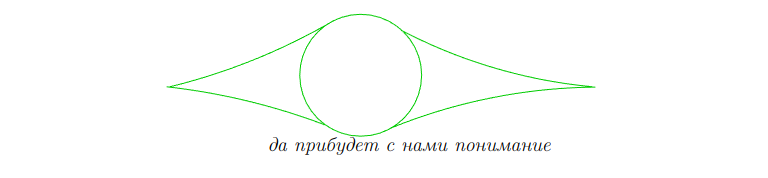
\includegraphics[width=13cm, height=3cm]{../img/ioda.png}
\end{center}

\section{Электроёмкость}
Экспериментально доказана следующая линейная зависимость:
\[q = C \phi\]

\define Здесь коэфициент C называется электроемкостью проводника.

Для сферы:
\[ C = 4 \pi \varepsilon_0 \varepsilon R\]
\begin{center}
    где $\varepsilon$ есть \textit{диэлектрическая проницаемость}
\end{center}
В системе СИ соотвественно: $[C = \frac{q}{\phi}] = \frac{\text{Кл}}{\text{В}} - \text{Фарад}$

\subsection{Конденсаторы}
Уединенные проводники, то есть те рядом с которыми нет других проводников, обладают малой емкостью.

Рассмотрим два проводника.Работа по перемещению от положительно заряженного проводника к отрицательно заряженному уменьшается, поскольку
такое перемещение совершается на r, а не на $\infty \Rightarrow$ уменьшается потенциал при сохранении заряда $\Rightarrow$
растет электроёмкость.

\define Устройство состоящее из таких проводников называется \textbf{конденсатором}.



\subsubsection{Плоский кондесатор}

\begin{center}
    \definecolor{ttttff}{rgb}{0.2,0.2,1}
    \definecolor{fftttt}{rgb}{1,0.2,0.2}
    \definecolor{qqccqq}{rgb}{0,0.8,0}
    \begin{tikzpicture}[line cap=round,line join=round,>=triangle 45,x=1.0cm,y=1.0cm]
        \clip(2.68,34.42) rectangle (9.54,41.25);
        \draw (4,23)-- (4,18);
        \draw [shift={(6.92,20.5)},color=qqccqq]  plot[domain=-1.51:1.51,variable=\t]({1*1.5*cos(\t r)+0*1.5*sin(\t r)},{0*1.5*cos(\t r)+1*1.5*sin(\t r)});
        \draw (7,22)-- (4.74,20.55);
        \draw (7,19)-- (4.74,20.55);
        \draw [color=fftttt](7.29,21.69) node[anchor=north west] {$+$};
        \draw [color=fftttt](7.58,21) node[anchor=north west] {$+$};
        \draw [color=fftttt](7.56,20.46) node[anchor=north west] {$+$};
        \draw [color=fftttt](7.41,20.04) node[anchor=north west] {$+$};
        \draw [color=fftttt](7.72,21.48) node[anchor=north west] {$+$};
        \draw [color=ttttff](5.16,20.94) node[anchor=north west] {$-$};
        \draw [color=ttttff](5.62,20.69) node[anchor=north west] {$-$};
        \draw [color=ttttff](5.54,21.27) node[anchor=north west] {$-$};
        \draw [shift={(4.28,20)},color=qqccqq]  plot[domain=0.67:1.69,variable=\t]({1*2.42*cos(\t r)+0*2.42*sin(\t r)},{0*2.42*cos(\t r)+1*2.42*sin(\t r)});
        \draw [shift={(4,18.79)},color=qqccqq]  plot[domain=0.95:1.57,variable=\t]({1*2.9*cos(\t r)+0*2.9*sin(\t r)},{0*2.9*cos(\t r)+1*2.9*sin(\t r)});
        \draw [shift={(4.47,21.39)},color=qqccqq]  plot[domain=4.44:5.4,variable=\t]({1*2.04*cos(\t r)+0*2.04*sin(\t r)},{0*2.04*cos(\t r)+1*2.04*sin(\t r)});
        \draw [shift={(4.92,20.88)},color=qqccqq]  plot[domain=4.29:5.52,variable=\t]({1*2.23*cos(\t r)+0*2.23*sin(\t r)},{0*2.23*cos(\t r)+1*2.23*sin(\t r)});
        \draw [color=qqccqq] (4.74,20.55)-- (4,20.57);
        \draw [color=fftttt] (4,41)-- (4,35);
        \draw [color=ttttff] (8,41)-- (8,35);
        \draw (3,38)-- (4,38);
        \draw (8,38)-- (9,38);
        \draw [->] (4,40) -- (7.74,40.02);
        \draw [->] (4,38.73) -- (7.74,38.75);
        \draw [->] (4,37.31) -- (7.64,37.37);
        \draw [->] (4,36.19) -- (7.7,36.25);
        \draw (5.85,41.18) node[anchor=north west] {$\vec E$};
        \draw [color=fftttt](3.54,41.16) node[anchor=north west] {$+$};
        \draw [color=ttttff](8.06,41.18) node[anchor=north west] {$-$};
        \draw (4.06,36.04) node[anchor=north west] {$\phi_1$};
        \draw (7.54,36.02) node[anchor=north west] {$\phi_2$};
    \end{tikzpicture}
\end{center}

\[q = C(\phi_1 - \phi_2) = CU\]

Далее: $Ed = U$, и в силу того что $E = \frac{\sigma}{\varepsilon \varepsilon_0}$

\[q = CEd = C\frac{\sigma}{\varepsilon \varepsilon_0} = C\frac{qd}{s\varepsilon \varepsilon_0} \Rightarrow 1 = C \frac{d}{s \varepsilon \varepsilon_0}\]

\[C = \frac{s\varepsilon_0\varepsilon}{d}\]

\begin{center}
    , где S- площадь пластины, d - расстояние между пластинами
    \newline
    \textbf{\textit{- электроемкость}}
\end{center}

Оптимальный способ увеличения электроемкости без увеличения размер пластины --- подбор других диэлектриков. то есть
изменение значения $\varepsilon$.

\define Диэлектрики удовлетворяющие свойствам:
\begin{enumerate}
    \item Высокая диэлектрическая проницаемость
    \item При исчезновении электрического поля у них остается некоторая остаточная поляризация.
\end{enumerate}
называются \textit{\textbf{сегнетоэлектриками}}.

\subsubsection{Цилиндрический кондесатор}

Вычислим заряд всего цилиндра с помощью площади боковой поверхности:
\[2 \pi R \cdot l \cdot \sigma = q \Rightarrow \sigma = \frac{q}{2 \pi R l}\]

\[\phi_1 - \phi_2 = \int_{r_1}^{r_2} \vec E d\vec r = \int_{r_1}^{r_2} \frac{\sigma R}{\varepsilon_0 \varepsilon} dr = \frac{\sigma R}{\varepsilon_0 \varepsilon}(ln r_2 - ln r_1)
    = \frac{\sigma R}{\varepsilon_0 \varepsilon} \cdot ln{|\frac{r_2}{r_1}|} = \frac{q \cdot R}{2 \pi R l \varepsilon_0 \varepsilon} ln{\frac{r_2}{r_1}}\]
Отсюда, в силу $q = C(\phi_1 - \phi_2) = CU \Rightarrow$:
\[C = \frac{\varepsilon \varepsilon_0 2 \pi l}{ln{\frac{r_2}{r_1}}}\]

Если $d = r_2 - r_1 << r_2$, то:
\[ln(1+ \frac{r_2 - r_1}{r_1}) \sim \frac{d}{r_1}\]
Тогда заменяя:
\[C = \frac{\varepsilon \varepsilon_0 2 \pi l r_1}{d} \approx \frac{\varepsilon \varepsilon_0 s}{d}\]
Равенство выше верно для разности размеров много меньше, чем радиус большего цилиндра.

\begin{center}
    \definecolor{ttttff}{rgb}{0.2,0.2,1}
    \definecolor{fftttt}{rgb}{1,0.2,0.2}
    \definecolor{qqccqq}{rgb}{0,0.8,0}
    \begin{tikzpicture}[line cap=round,line join=round,>=triangle 45,x=1.0cm,y=1.0cm]
        \clip(2.91,36.73) rectangle (10.28,42.08);
        \draw (4,23)-- (4,18);
        \draw [shift={(6.92,20.5)},color=qqccqq]  plot[domain=-1.51:1.51,variable=\t]({1*1.5*cos(\t r)+0*1.5*sin(\t r)},{0*1.5*cos(\t r)+1*1.5*sin(\t r)});
        \draw (7,22)-- (4.74,20.55);
        \draw (7,19)-- (4.74,20.55);
        \draw [color=fftttt](7.29,21.69) node[anchor=north west] {$+$};
        \draw [color=fftttt](7.58,21) node[anchor=north west] {$+$};
        \draw [color=fftttt](7.56,20.46) node[anchor=north west] {$+$};
        \draw [color=fftttt](7.41,20.04) node[anchor=north west] {$+$};
        \draw [color=fftttt](7.72,21.48) node[anchor=north west] {$+$};
        \draw [color=ttttff](5.16,20.94) node[anchor=north west] {$-$};
        \draw [color=ttttff](5.62,20.69) node[anchor=north west] {$-$};
        \draw [color=ttttff](5.54,21.27) node[anchor=north west] {$-$};
        \draw [shift={(4.28,20)},color=qqccqq]  plot[domain=0.67:1.69,variable=\t]({1*2.42*cos(\t r)+0*2.42*sin(\t r)},{0*2.42*cos(\t r)+1*2.42*sin(\t r)});
        \draw [shift={(4,18.79)},color=qqccqq]  plot[domain=0.95:1.57,variable=\t]({1*2.9*cos(\t r)+0*2.9*sin(\t r)},{0*2.9*cos(\t r)+1*2.9*sin(\t r)});
        \draw [shift={(4.47,21.39)},color=qqccqq]  plot[domain=4.44:5.4,variable=\t]({1*2.04*cos(\t r)+0*2.04*sin(\t r)},{0*2.04*cos(\t r)+1*2.04*sin(\t r)});
        \draw [shift={(4.92,20.88)},color=qqccqq]  plot[domain=4.29:5.52,variable=\t]({1*2.23*cos(\t r)+0*2.23*sin(\t r)},{0*2.23*cos(\t r)+1*2.23*sin(\t r)});
        \draw [color=qqccqq] (4.74,20.55)-- (4,20.57);
        \draw(5.65,39.21) circle (1.63cm);
        \draw [color=qqccqq] (5.6,39.21) circle (0.87cm);
        \draw (5.08,40.74)-- (7.76,41.47);
        \draw (7.27,39.41)-- (9,40);
        \draw [shift={(7.54,40.02)}] plot[domain=-0.02:1.42,variable=\t]({1*1.46*cos(\t r)+0*1.46*sin(\t r)},{0*1.46*cos(\t r)+1*1.46*sin(\t r)});
        \draw (6.12,37.64)-- (8.7,38.68);
        \draw [shift={(6.3,39.92)}] plot[domain=-0.48:0.03,variable=\t]({1*2.7*cos(\t r)+0*2.7*sin(\t r)},{0*2.7*cos(\t r)+1*2.7*sin(\t r)});
        \draw [->,color=qqccqq] (5.6,39.23) -- (5.79,40.06);
        \draw [->] (5.6,39.23) -- (7,38.28);
        \draw (5.27,40.02) node[anchor=north west] {$r_1$};
        \draw (6.58,39.12) node[anchor=north west] {$r_2$};
        \draw (7.85,40.31) node[anchor=north west] {$l$};
    \end{tikzpicture}
\end{center}

\subsubsection{Сферический конденсатор}
Рассмотрим сферический конденсатор:
\[C = \frac{4 \pi \varepsilon \varepsilon_0 R_1 R_2}{(R_1 - R_2)}\]
\begin{center}
    где $R_1 \approx R_2$
\end{center}
Если $d = R_1 -R_2 << R_2$, то можно использовать:
\[C = \frac{\varepsilon \varepsilon_0 s}{d}\]

\subsubsection{Соединение конденсаторов}

Предельное значение напряжения конденсатора $U_{max}$.

Если превысить это значение может случится так называемый \textit{пробой конденсаторов.}

Таким образом, получаем что у конденсатора можно выделить две характеристики: $U_{max}$ и $C$. Часто требуется использовать несколько
конденсаторов объединяя их в конденсаторные батареи.

\vspace{5px}

Соединения могут быть двух типов:
\begin{enumerate}
    \item \textit{\textbf{Параллельные:}}
          \begin{center}
              \definecolor{ttttff}{rgb}{0.2,0.2,1}
              \definecolor{fftttt}{rgb}{1,0.2,0.2}
              \definecolor{qqccqq}{rgb}{0,0.8,0}
              \begin{tikzpicture}[line cap=round,line join=round,>=triangle 45,x=1.0cm,y=1.0cm]
                  \clip(2.27,35.89) rectangle (7.89,41.18);
                  \draw (4,23)-- (4,18);
                  \draw [shift={(6.92,20.5)},color=qqccqq]  plot[domain=-1.51:1.51,variable=\t]({1*1.5*cos(\t r)+0*1.5*sin(\t r)},{0*1.5*cos(\t r)+1*1.5*sin(\t r)});
                  \draw (7,22)-- (4.74,20.55);
                  \draw (7,19)-- (4.74,20.55);
                  \draw [color=fftttt](7.29,21.69) node[anchor=north west] {$+$};
                  \draw [color=fftttt](7.58,21) node[anchor=north west] {$+$};
                  \draw [color=fftttt](7.56,20.46) node[anchor=north west] {$+$};
                  \draw [color=fftttt](7.41,20.04) node[anchor=north west] {$+$};
                  \draw [color=fftttt](7.72,21.48) node[anchor=north west] {$+$};
                  \draw [color=ttttff](5.16,20.94) node[anchor=north west] {$-$};
                  \draw [color=ttttff](5.62,20.69) node[anchor=north west] {$-$};
                  \draw [color=ttttff](5.54,21.27) node[anchor=north west] {$-$};
                  \draw [shift={(4.28,20)},color=qqccqq]  plot[domain=0.67:1.69,variable=\t]({1*2.42*cos(\t r)+0*2.42*sin(\t r)},{0*2.42*cos(\t r)+1*2.42*sin(\t r)});
                  \draw [shift={(4,18.79)},color=qqccqq]  plot[domain=0.95:1.57,variable=\t]({1*2.9*cos(\t r)+0*2.9*sin(\t r)},{0*2.9*cos(\t r)+1*2.9*sin(\t r)});
                  \draw [shift={(4.47,21.39)},color=qqccqq]  plot[domain=4.44:5.4,variable=\t]({1*2.04*cos(\t r)+0*2.04*sin(\t r)},{0*2.04*cos(\t r)+1*2.04*sin(\t r)});
                  \draw [shift={(4.92,20.88)},color=qqccqq]  plot[domain=4.29:5.52,variable=\t]({1*2.23*cos(\t r)+0*2.23*sin(\t r)},{0*2.23*cos(\t r)+1*2.23*sin(\t r)});
                  \draw [color=qqccqq] (4.74,20.55)-- (4,20.57);
                  \draw (3,40)-- (7,40);
                  \draw (7,39)-- (7,40);
                  \draw (3,39)-- (3,40);
                  \draw (2.5,39)-- (3.54,39);
                  \draw (6.6,38.98)-- (7.52,38.98);
                  \draw (5,40)-- (5,39);
                  \draw (4.56,38.98)-- (5.58,38.98);
                  \draw (2.5,38)-- (3.54,38);
                  \draw (3,38)-- (3,37);
                  \draw (3,37)-- (7,37);
                  \draw (7,38)-- (7,37);
                  \draw (6.62,37.98)-- (7.56,37.98);
                  \draw (4.56,37.98)-- (5.52,37.98);
                  \draw (5,37.98)-- (5,37);
                  \draw (5,40)-- (5,41);
                  \draw (5,37)-- (4.97,35.87);
                  \draw [color=fftttt](5.2,40.79) node[anchor=north west] {$+$};
                  \draw [color=ttttff](5.12,36.96) node[anchor=north west] {$-$};
                  \draw (2.79,38.89) node[anchor=north west] {$C_1$};
                  \draw (4.85,38.95) node[anchor=north west] {$C_2$};
                  \draw (5.81,38.96) node[anchor=north west] {$\dots$};
                  \draw (6.91,38.96) node[anchor=north west] {$C_n$};
                  \draw (2.52,39.83) node[anchor=north west] {$\phi_1$};
                  \draw (4.66,39.77) node[anchor=north west] {$\phi_1$};
                  \draw (6.56,39.71) node[anchor=north west] {$\phi_1$};
                  \draw (2.54,38.1) node[anchor=north west] {$\phi_2$};
                  \draw (4.56,38.04) node[anchor=north west] {$\phi_2$};
                  \draw (6.6,38.04) node[anchor=north west] {$\phi_2$};
              \end{tikzpicture}
          \end{center}
          \[U_1 = U_2 = \ldots = U_n = U\]
          \[q = \sum_{i = 1}^{n} q_i = \sum_{i = 1}^{n}(C_i \cdot U) = U \sum_{i = 1}^{n} C_i\]
          Для параллельного соединения:
          \[C = \sum_{i = 1}^{n} C_i\]
          При этом
          \[U_{max} = min_{(i = 1,n)} U_{i_{max}}\]
    \item \textit{\textbf{Последовательные}}
          \begin{center}
              \definecolor{ttttff}{rgb}{0.2,0.2,1}
              \definecolor{fftttt}{rgb}{1,0.2,0.2}
              \definecolor{qqccqq}{rgb}{0,0.8,0}
              \begin{tikzpicture}[line cap=round,line join=round,>=triangle 45,x=1.0cm,y=1.0cm]
                  \clip(2.61,54.88) rectangle (5.46,62.12);
                  \draw (4,23)-- (4,18);
                  \draw [shift={(6.92,20.5)},color=qqccqq]  plot[domain=-1.51:1.51,variable=\t]({1*1.5*cos(\t r)+0*1.5*sin(\t r)},{0*1.5*cos(\t r)+1*1.5*sin(\t r)});
                  \draw (7,22)-- (4.74,20.55);
                  \draw (7,19)-- (4.74,20.55);
                  \draw [color=fftttt](7.3,21.67) node[anchor=north west] {$+$};
                  \draw [color=fftttt](7.59,20.98) node[anchor=north west] {$+$};
                  \draw [color=fftttt](7.56,20.44) node[anchor=north west] {$+$};
                  \draw [color=fftttt](7.42,20.01) node[anchor=north west] {$+$};
                  \draw [color=fftttt](7.71,21.45) node[anchor=north west] {$+$};
                  \draw [color=ttttff](5.16,20.91) node[anchor=north west] {$-$};
                  \draw [color=ttttff](5.63,20.67) node[anchor=north west] {$-$};
                  \draw [color=ttttff](5.54,21.24) node[anchor=north west] {$-$};
                  \draw [shift={(4.28,20)},color=qqccqq]  plot[domain=0.67:1.69,variable=\t]({1*2.42*cos(\t r)+0*2.42*sin(\t r)},{0*2.42*cos(\t r)+1*2.42*sin(\t r)});
                  \draw [shift={(4,18.79)},color=qqccqq]  plot[domain=0.95:1.57,variable=\t]({1*2.9*cos(\t r)+0*2.9*sin(\t r)},{0*2.9*cos(\t r)+1*2.9*sin(\t r)});
                  \draw [shift={(4.47,21.39)},color=qqccqq]  plot[domain=4.44:5.4,variable=\t]({1*2.04*cos(\t r)+0*2.04*sin(\t r)},{0*2.04*cos(\t r)+1*2.04*sin(\t r)});
                  \draw [shift={(4.92,20.88)},color=qqccqq]  plot[domain=4.29:5.52,variable=\t]({1*2.23*cos(\t r)+0*2.23*sin(\t r)},{0*2.23*cos(\t r)+1*2.23*sin(\t r)});
                  \draw [color=qqccqq] (4.74,20.55)-- (4,20.57);
                  \draw (3,40)-- (7,40);
                  \draw (7,39)-- (7,40);
                  \draw (3,39)-- (3,40);
                  \draw (2.5,39)-- (3.54,39);
                  \draw (6.6,38.98)-- (7.52,38.98);
                  \draw (5,40)-- (5,39);
                  \draw (4.56,38.98)-- (5.58,38.98);
                  \draw (2.5,38)-- (3.54,38);
                  \draw (3,38)-- (3,37);
                  \draw (3,37)-- (7,37);
                  \draw (7,38)-- (7,37);
                  \draw (6.62,37.98)-- (7.56,37.98);
                  \draw (4.56,37.98)-- (5.52,37.98);
                  \draw (5,37.98)-- (5,37);
                  \draw (5,40)-- (5,41);
                  \draw (5,37)-- (4.97,35.87);
                  \draw (2.8,38.86) node[anchor=north west] {$C_1$};
                  \draw (4.85,38.93) node[anchor=north west] {$C_2$};
                  \draw (5.82,38.95) node[anchor=north west] {$\dots$};
                  \draw (6.91,38.95) node[anchor=north west] {$C_n$};
                  \draw (2.52,39.82) node[anchor=north west] {$\phi_1$};
                  \draw (4.66,39.75) node[anchor=north west] {$\phi_1$};
                  \draw (6.57,39.69) node[anchor=north west] {$\phi_1$};
                  \draw (2.54,38.08) node[anchor=north west] {$\phi_2$};
                  \draw (4.57,38.01) node[anchor=north west] {$\phi_2$};
                  \draw (6.6,38.01) node[anchor=north west] {$\phi_2$};
                  \draw (4,62)-- (4,61);
                  \draw [color=fftttt] (3,61)-- (5,61);
                  \draw [color=ttttff] (3,60)-- (5,60);
                  \draw (4,60)-- (4,59);
                  \draw [color=fftttt] (3,59)-- (5,59);
                  \draw [color=ttttff] (3,58)-- (5,58);
                  \draw (3.99,58)-- (4,57);
                  \draw [color=fftttt] (3,57)-- (5,57);
                  \draw [color=ttttff] (3,56)-- (5,56);
                  \draw (4,56)-- (4,55);
                  \draw [color=fftttt](2.92,61.69) node[anchor=north west] {$+$};
                  \draw [color=fftttt](3.16,59.54) node[anchor=north west] {$+$};
                  \draw [color=fftttt](3.2,57.56) node[anchor=north west] {$+$};
                  \draw [color=ttttff](3.03,60.56) node[anchor=north west] {$-$};
                  \draw [color=ttttff](2.97,58.65) node[anchor=north west] {$-$};
                  \draw [color=ttttff](3.03,56.6) node[anchor=north west] {$-$};
                  \draw (4.81,60.99) node[anchor=north west] {$C_1$};
                  \draw (4.88,59.97) node[anchor=north west] {$C_2$};
                  \draw (4.9,57.99) node[anchor=north west] {$C_3$};
                  \draw (4.9,55.89) node[anchor=north west] {$C_n$};
                  \draw (4.62,56.88) node[anchor=north west] {$\ldots$};
              \end{tikzpicture}
          \end{center}
          \[q_1 =q_2 = \ldots = q_n = q\]
          \[U = \frac{q}{C}\]
          \[U = \sum_{i = 1}^{n} U_i = \sum_{i=1}^{n} \frac{q}{C_i} \Rightarrow \frac{1}{C} = \sum_{i=1}^{n}\frac{1}{C_i}\]
          \begin{center}
              если все конденсаторы одинаковые
          \end{center}
          \[U_{max} = n \cdot U_{i_{max}}\]
          \begin{center}
              если ёмкость конденсаторов одинаковая
          \end{center}
\end{enumerate}

\section{Энергия электрического поля}
\subsection{Энергия системы зарядов}
Возьмем два заряда, $q_1$ $q_2$,

Обозначим потенциал создаваемый первым зарядом в точке $q_2$ назовем $\phi_2$, и наоборот потенциал вторым зарядом в точке $q_1$ назовем $\phi_1$.

Энергия взаимодействия зарядов:
\[W_{12} = \frac{1}{4 \pi \varepsilon_0} \frac{q_1 \cdot q_2}{r_{12}} = (\frac{1}{4 \pi \varepsilon_0} \frac{q_2}{r_{12}}) \cdot q_1\]
\[W_{12} = \phi_2 q_2 = \phi_1 q_1 = \frac{1}{2} (\phi_1 q_1 + \phi_2 q_2)\]

К этой системе добавим заряд $q_3$ и добавим обозначение $\phi_3$ - потенциал который создают заряды $q_1$ $q_2$ в точке $q_3$,
тогда выразим энергию заряда $q_3$ в этом поле:
\[W_3 = \phi_3 q_3 = \frac{1}{4 \pi \varepsilon_0} \cdot \frac{q_1 \cdot q_3}{r_{13}} + \frac{1}{4 \pi \varepsilon_0} \cdot \frac{q_2 \cdot q_3}{r_{23}}\]

Тогда можем получить полную формулу энергии трех зарядов в этой системе:
\[W = W_{12} + W_{13} + W_{23} = \frac{1}{4 \pi \varepsilon_0} (\frac{q_1 \cdot q_2}{r_{12}} + \frac{q_1 \cdot q_3}{r_{13}}+ \frac{q_2 \cdot q_3}{r_{23}}) = \]
\[ \frac{1}{2}\frac{1}{4 \pi \varepsilon_0}(\frac{q_1 \cdot q_2}{r_{12}} + \frac{q_1 \cdot q_3}{r_{13}}+ \frac{q_2 \cdot q_3}{r_{23}} + \frac{q_2 \cdot q_1}{r_{21}} + \frac{q_3 \cdot q_1}{r_{31}}+ \frac{q_3 \cdot q_2}{r_{32}}) = \]
\[ \frac{1}{2}(\frac{q_1}{4 \pi \varepsilon_0}(\frac{q_2}{r_{12}} + \frac{q_3}{r_{13}}) + \frac{q_2}{4 \pi \varepsilon_0}(\frac{q_1}{r_{12}} + \frac{q_3}{r_{13}}) + \frac{q_3}{4 \pi \varepsilon_0}(\frac{q_1}{r_{12}} + \frac{q_2}{r_{13}}) ) = \]
\[ \frac{1}{2} (q_1 \phi_1 + q_2 \phi_2  + q_3 \phi_3) \]

Продолжая аналогичным образом получим итоговую энергию системы зарядов:
\[W = \frac{1}{2} \sum_{i=1}^{N} \phi_i q_i\]

где потенциал $\phi_i$ создаваемый в точке $q_i$ всеми остальными зарядами

\subsection{Энергия заряженного проводника}
Возьмем проводник. Поскольку заряд распределен на поверхности проводника, так разобьем всю поверхность на маленькие кусочки.
Важно отметить что поверхность проводника есть эквипотенциальная поверхность, тогда посчитаем энергию зарядов на этих кусочках:
\[W = \frac{1}{2} \sum_{i=1}^{N} (\phi_i \Delta q_i) = \frac{1}{2} \sum_{i=1}^{N} (\phi \Delta q_i) =
    \frac{1}{2} \phi \sum_{i=1}^{N} (\Delta q_i) = \frac{1}{2} \phi q = \frac{1}{2} \phi^2 \cdot C = \frac{q^2}{2C}
\]
\subsection{Энергия заряженного кондесатора}

\[ W = \frac{1}{2}\phi_1 q + \frac{1}{2}\phi_2 -q = \frac{1}{2}q (\phi_1 - \phi_2) = \frac{1}{2} q \Delta \phi
    = \frac{1}{2} q U = \frac{1}{2} C U^2 =\frac{1}{2} \frac{q^2}{C}\]
\subsection{Энергия электрического поля}
Наличие диэлектрика влияет на общую энергию электрического поля.

Будем расматривать плоский конденсатор, подставим в эту формулы выражение для емкости:
\[ W = \frac{1}{2} C \cdot U^2 = \frac{1}{2} \frac{\varepsilon \varepsilon_0 S}{d} \cdot U^2 = \frac{1}{2} \frac{\varepsilon \varepsilon_0 S}{d} \cdot E^2 d^2 = \frac{1}{2}(\varepsilon \varepsilon_0 E^2) S \cdot d =
    \frac{\varepsilon \varepsilon_ 0 E^2}{2} \cdot V\]
\begin{center}
    где $V$ - объем конденсатора
\end{center}

Объемная плотность энергии электрического поля:
\[w = \frac{W}{V} = \frac{\varepsilon \varepsilon_ 0 E^2}{2} = \frac{D E}{2} = \frac{D^2}{2} \varepsilon \varepsilon_0\]
В анизотропных средах заметим что направления D и E не совпадают тогда берем скалярное поризведение векторов D и E:
\[w = \frac{\vec D \cdot \vec E}{2} = \frac{\vec E (\varepsilon_0 \vec E + \vec P)}{2} = \frac{\varepsilon_0 E^2}{2} + \frac{\vec E \vec P}{2}\]
\begin{center}
    $\frac{\varepsilon_0 E^2}{2}$ - энергия электрического поля в вакууме,
    \newline
    $\frac{\vec E \vec P}{2}$ - энергия поляризации
\end{center}

\section{Постоянный электрический ток}

\define \textbf{Электрическим током} называется упорядоченное движение заряженных частиц.

За направление тока принимается движения положительно заряженных частиц.

\define Такое движение принято характеризовать \textbf{силой тока}  --- заряд прошедший через сечение проводника за единицу времени.
\[i = \frac{dq}{dt} = \frac{dq ^{+}}{dt} + \frac{dq ^{-}}{dt}\]
\begin{center}
    --- сила переменного электрического тока.
\end{center}


Поскольку наши частицы есть свободные частицы, то движутся они хаотично. Тогда можем определить скорость хаотического движения зарядов $\vec v$,
а $\vec u$ - скрость упорядоченного движения заряда.

Рассматривая ток внутри материала вводят \textit{величину плотности тока.}

Сила тока величина \textit{скалярная}, плотность тока величина \textit{векторная} --- $\vec \iota = \frac{I}{S}$,
плотность тока всегда направлена по линии движения тока. S есть площадь перпендикулярная направлению тока.

\[i = \iint_{s} \vec \iota \cdot \vec n ds\]

\[\vec \iota = q \cdot n \cdot \vec u = q^{+} \cdot n^{+} \cdot \vec u^{+} + q^{-} \cdot n^{-} \cdot \vec u^{-}\]
В системе СИ:

[I] = А (Ампер)

В свою очередь, через Амперы может вычислить и другие величины:
\begin{center}
    Кл = $A \cdot c$
    В = $\frac{\text{Дж}}{\text{Кл}}$ = $\frac{\text{кг} \cdot \text{м}^2}{\text{A} \cdot \text{с}^2}$
\end{center}

\subsection{Электродвижущая сила}
Возьмем уединенный проводник и поместим его в электрическое поле. Движение частиц по такому проводнику будет недолгим.
\begin{center}
    \definecolor{zzttqq}{rgb}{0.6,0.2,0}
    \definecolor{ttttff}{rgb}{0.2,0.2,1}
    \definecolor{fftttt}{rgb}{1,0.2,0.2}
    \definecolor{qqccqq}{rgb}{0,0.8,0}
    \begin{tikzpicture}[line cap=round,line join=round,>=triangle 45,x=1.0cm,y=1.0cm]
        \clip(0.87,59.87) rectangle (9.6,61.9);
        \fill[color=zzttqq,fill=zzttqq,fill opacity=0.1] (1.98,61.55) -- (9,61.57) -- (9,61) -- (2,61) -- cycle;
        \draw (4,23)-- (4,18);
        \draw [shift={(6.92,20.5)},color=qqccqq]  plot[domain=-1.51:1.51,variable=\t]({1*1.5*cos(\t r)+0*1.5*sin(\t r)},{0*1.5*cos(\t r)+1*1.5*sin(\t r)});
        \draw (7,22)-- (4.74,20.55);
        \draw (7,19)-- (4.74,20.55);
        \draw [color=fftttt](7.3,21.67) node[anchor=north west] {$+$};
        \draw [color=fftttt](7.59,20.98) node[anchor=north west] {$+$};
        \draw [color=fftttt](7.56,20.44) node[anchor=north west] {$+$};
        \draw [color=fftttt](7.42,20.01) node[anchor=north west] {$+$};
        \draw [color=fftttt](7.71,21.45) node[anchor=north west] {$+$};
        \draw [color=ttttff](5.16,20.91) node[anchor=north west] {$-$};
        \draw [color=ttttff](5.63,20.67) node[anchor=north west] {$-$};
        \draw [color=ttttff](5.54,21.24) node[anchor=north west] {$-$};
        \draw [shift={(4.28,20)},color=qqccqq]  plot[domain=0.67:1.69,variable=\t]({1*2.42*cos(\t r)+0*2.42*sin(\t r)},{0*2.42*cos(\t r)+1*2.42*sin(\t r)});
        \draw [shift={(4,18.79)},color=qqccqq]  plot[domain=0.95:1.57,variable=\t]({1*2.9*cos(\t r)+0*2.9*sin(\t r)},{0*2.9*cos(\t r)+1*2.9*sin(\t r)});
        \draw [shift={(4.47,21.39)},color=qqccqq]  plot[domain=4.44:5.4,variable=\t]({1*2.04*cos(\t r)+0*2.04*sin(\t r)},{0*2.04*cos(\t r)+1*2.04*sin(\t r)});
        \draw [shift={(4.92,20.88)},color=qqccqq]  plot[domain=4.29:5.52,variable=\t]({1*2.23*cos(\t r)+0*2.23*sin(\t r)},{0*2.23*cos(\t r)+1*2.23*sin(\t r)});
        \draw [color=qqccqq] (4.74,20.55)-- (4,20.57);
        \draw (3,40)-- (7,40);
        \draw (7,39)-- (7,40);
        \draw (3,39)-- (3,40);
        \draw (2.5,39)-- (3.54,39);
        \draw (6.6,38.98)-- (7.52,38.98);
        \draw (5,40)-- (5,39);
        \draw (4.56,38.98)-- (5.58,38.98);
        \draw (2.5,38)-- (3.54,38);
        \draw (3,38)-- (3,37);
        \draw (3,37)-- (7,37);
        \draw (7,38)-- (7,37);
        \draw (6.62,37.98)-- (7.56,37.98);
        \draw (4.56,37.98)-- (5.52,37.98);
        \draw (5,37.98)-- (5,37);
        \draw (5,40)-- (5,41);
        \draw (5,37)-- (4.97,35.87);
        \draw (2.8,38.86) node[anchor=north west] {$C_1$};
        \draw (4.85,38.93) node[anchor=north west] {$C_2$};
        \draw (5.82,38.95) node[anchor=north west] {$\dots$};
        \draw (6.91,38.95) node[anchor=north west] {$C_n$};
        \draw (2.52,39.82) node[anchor=north west] {$\phi_1$};
        \draw (4.66,39.75) node[anchor=north west] {$\phi_1$};
        \draw (6.57,39.69) node[anchor=north west] {$\phi_1$};
        \draw (2.54,38.08) node[anchor=north west] {$\phi_2$};
        \draw (4.57,38.01) node[anchor=north west] {$\phi_2$};
        \draw (6.6,38.01) node[anchor=north west] {$\phi_2$};
        \draw [color=zzttqq] (1.98,61.55)-- (9,61.57);
        \draw [color=zzttqq] (9,61.57)-- (9,61);
        \draw [color=zzttqq] (9,61)-- (2,61);
        \draw [color=zzttqq] (2,61)-- (1.98,61.55);
        \draw (2,61.64) node[anchor=north west] {$-$};
        \draw (8.53,61.67) node[anchor=north west] {$+$};
        \draw [shift={(4.54,73.01)}] plot[domain=4.51:5.07,variable=\t]({1*12.81*cos(\t r)+0*12.81*sin(\t r)},{0*12.81*cos(\t r)+1*12.81*sin(\t r)});
        \draw [shift={(1.92,60.87)}] plot[domain=1.45:4.7,variable=\t]({1*0.4*cos(\t r)+0*0.4*sin(\t r)},{0*0.4*cos(\t r)+1*0.4*sin(\t r)});
        \draw [color=fftttt](6.43,60.94) node[anchor=north west] {$+$};
        \draw [color=fftttt](5.72,60.8) node[anchor=north west] {$+$};
        \draw [color=fftttt](4.62,60.73) node[anchor=north west] {$+$};
        \draw [color=fftttt](3.58,60.77) node[anchor=north west] {$+$};
        \draw [color=fftttt](2.59,60.86) node[anchor=north west] {$+$};
    \end{tikzpicture}
\end{center}
Так для того чтобы движение частиц продолжилось нужны посторонние силы, которые заставляют заряженные частицы переместиться в начало:

Эти сторонние силы совершают работу по переносу заряда.

\vspace{5px}

\define Величина равная работе сторонних сил, деленная на велиичну перенесенного заряда называется \textbf{электродвижующей силы.}

\[\mathscr{E} = \frac{A}{q}\]

В системе СИ: [$\mathscr{E}$] = В

Рассмотрим некоторый контур:
\begin{center}
    \definecolor{ttccqq}{rgb}{0.2,0.8,0}
    \begin{tikzpicture}[line cap=round,line join=round,>=triangle 45,x=1.0cm,y=1.0cm]
        \clip(6.11,10.59) rectangle (10.35,12.19);
        \fill[color=ttccqq,fill=ttccqq,fill opacity=0.1] (7,12) -- (9.5,12) -- (9.5,11.5) -- (7,11.5) -- cycle;
        \draw [color=ttccqq] (7,12)-- (9.5,12);
        \draw [color=ttccqq] (9.5,12)-- (9.5,11.5);
        \draw [color=ttccqq] (9.5,11.5)-- (7,11.5);
        \draw [color=ttccqq] (7,11.5)-- (7,12);
        \draw (9.5,11.75)-- (10,11.75);
        \draw (10,11.75)-- (10,11);
        \draw (10,11)-- (8.27,11);
        \draw (7,11.76)-- (6.5,11.76);
        \draw (6.5,11.76)-- (6.5,11);
        \draw (6.5,11)-- (8,11);
        \draw (8,11.15)-- (7.99,10.82);
        \draw (8.26,11.22)-- (8.25,10.71);
        \draw (7.7,11.51) node[anchor=north west] {$-$};
        \draw (8.18,11.54) node[anchor=north west] {$+$};
    \end{tikzpicture}
\end{center}

Посчитаем работу сторонних сил по такому замкнутому контуру:

\[A = \oint \vec F_{st} d \vec l + \oint \vec E d \vec l  = \oint \vec F_{st} d \vec l\]

Вводя напряженность поля создаваемого стороними силами:
\[\vec E_{st} = \frac{\vec F_{st}}{q}\]
Получаем что:
\[A = q \oint \vec E_{st} d \vec l \Rightarrow \]
\[\mathscr{E} = \oint \vec E_{st} dl\]

\vspace{6px}

Рассмотрим другой проводник на который действует ЭДС:

\begin{center}
    \definecolor{ttccqq}{rgb}{0.2,0.8,0}
    \begin{tikzpicture}[line cap=round,line join=round,>=triangle 45,x=1.5362991308223641cm,y=2.088068428879986cm]
        \clip(9.04,5.21) rectangle (12.77,6.12);
        \fill[color=ttccqq,fill=ttccqq,fill opacity=0.1] (7,12) -- (9.5,12) -- (9.5,11.5) -- (7,11.5) -- cycle;
        \fill[color=ttccqq,fill=ttccqq,fill opacity=0.1] (9.28,5.7) -- (9.29,5.5) -- (10.8,5.5) -- (10.8,5.71) -- cycle;
        \fill[color=ttccqq,fill=ttccqq,fill opacity=0.1] (11.02,5.72) -- (11.03,5.52) -- (12.53,5.52) -- (12.53,5.73) -- cycle;
        \draw [color=ttccqq] (7,12)-- (9.5,12);
        \draw [color=ttccqq] (9.5,12)-- (9.5,11.5);
        \draw [color=ttccqq] (9.5,11.5)-- (7,11.5);
        \draw [color=ttccqq] (7,11.5)-- (7,12);
        \draw (9.5,11.75)-- (10,11.75);
        \draw (10,11.75)-- (10,11);
        \draw (10,11)-- (8.27,11);
        \draw (7,11.76)-- (6.5,11.76);
        \draw (6.5,11.76)-- (6.5,11);
        \draw (6.5,11)-- (8,11);
        \draw (8,11.15)-- (7.99,10.82);
        \draw (8.26,11.22)-- (8.25,10.71);
        \draw (7.9,11.5) node[anchor=north west] {$-$};
        \draw (8.19,11.52) node[anchor=north west] {$+$};
        \draw [color=ttccqq] (9.28,5.7)-- (9.29,5.5);
        \draw [color=ttccqq] (9.29,5.5)-- (10.8,5.5);
        \draw [color=ttccqq] (10.8,5.5)-- (10.8,5.71);
        \draw [color=ttccqq] (10.8,5.71)-- (9.28,5.7);
        \draw [color=ttccqq] (11.02,5.72)-- (11.03,5.52);
        \draw [color=ttccqq] (11.03,5.52)-- (12.53,5.52);
        \draw [color=ttccqq] (12.53,5.52)-- (12.53,5.73);
        \draw [color=ttccqq] (12.53,5.73)-- (11.02,5.72);
        \draw (11.02,5.93)-- (11.01,5.32);
        \draw (9.18,5.55) node[anchor=north west] {$\phi_1$};
        \draw (9.17,6) node[anchor=north west] {$A$};
        \draw (12.44,6.02) node[anchor=north west] {$B$};
        \draw (12.4,5.58) node[anchor=north west] {$\phi_2$};
        \draw (10.72,6.18) node[anchor=north west] {$E$};
        \draw (10.8,5.8)-- (10.8,5.4);
    \end{tikzpicture}
\end{center}

Посчитаем работу всех силы произведенную на этом участке

\[A = \int_{a}^{b} \vec F_{st} d \vec l + \int_{a}^{b} \vec F d \vec l = q \int \vec E_{st} d \vec l + q \oint \vec E d \vec l = q \cdot \mathscr{E}_{ab} + q \cdot (\phi_1 - \phi_2)\]

\define Падением напряжения называется величина равная:
\[\frac{A}{q} = U = \mathscr{E}_{ab} + (\phi_1 - \phi_2)\]
В общем говоря, разность потенциалов и падение напряжение не одно и то же, они совпадают тогда и только тогда $\mathscr{E}_{ab}$ отсутствует.

\vspace{5px}

\define Проводник на котором нет ЭДС называется \textit{однородным}, если ЭДС имеется называется \textit{неоднородным.}

\subsection{Закон Ома сопротивления проводников}

Сила тока и приложенное напряжение(и разность потенциалов) в однородном проводнике вычисляется как:
\[I = \frac{U}{R}\]
\begin{center}
    где R - сопротивление проводника
\end{center}


Экспериментально было показано, что сопротивление зависит от площади, длины и свойств материала проводника, тогда верна формула:
\[R = \rho \frac{l}{s}\]
\begin{center}
    где $\rho$  называется \textit{удельным сопротивлением проводника}
\end{center}
\define Величина обратная к сопротивлению проводника: $\frac{1}{\rho} = \sigma$ называется \textbf{удельной проводимостью.}

\begin{center}

    \definecolor{ttccqq}{rgb}{0.2,0.8,0}
    \definecolor{ffqqqq}{rgb}{1,0,0}
    \begin{tikzpicture}[line cap=round,line join=round,>=triangle 45,x=2.5008306419693462cm,y=2.51583894838904cm]
        \clip(5.44,7.69) rectangle (8.11,9.01);
        \draw [color=ffqqqq,fill=ffqqqq,fill opacity=0.05] (6.13,8.22) ellipse (0.78cm and 0.79cm);
        \draw [color=ttccqq] (6,8.5)-- (7.3,8.82);
        \draw (6.17,7.91)-- (7.49,8.26);
        \draw [shift={(7.45,8.56)}] plot[domain=-1.42:2.08,variable=\t]({1*0.3*cos(\t r)+0*0.3*sin(\t r)},{0*0.3*cos(\t r)+1*0.3*sin(\t r)});
        \draw [color=ttccqq](6.59,9.01) node[anchor=north west] {$dl$};
        \draw [color=ffqqqq](5.98,8.37) node[anchor=north west] {$dS$};
    \end{tikzpicture}

\end{center}

Будем считать, что на $dl$ напряженность постоянна, тогда:

\[U = \vec E \cdot d \vec l\]

При малых значениях длины проводника можем вычислить:
\[I = \iota ds \]
\[ \iota ds = \frac{E dl}{\rho \frac{dl}{ds}} =  \frac{E}{\rho} ds \Rightarrow\]

\[\iota = \frac{E}{\rho}\]

\define Такую запись называют \textbf{диференциальной записью закона Ома}

Для металических проводников справедлива  зависимость сопротивления проводника от его температуры, тогда:

\[\rho = \rho_0 (1 + \alpha t)\]
\begin{center}
    где $\alpha = \frac{1}{273}$
\end{center}

Данная дифференциальная запись справедлива и для неоднородных проводнико с учетом наличия ЭДС , U воcпринимается как разность потенциалов $(U = \phi_1 - \phi_2)$, тогда
для неоднородных проводников справедливо:

\vspace{5px}

\makebox[\textwidth]{%
    \begin{minipage}{0.45\textwidth}
        \centering
        \textbf{Дифференциальная запись:}\\[2mm]
        $\displaystyle j = \frac{1}{\rho}\Bigl(\vec{E} + \vec{E}_{st}\Bigr)$
    \end{minipage}%
    \hfill
    \begin{minipage}{0.45\textwidth}
        \centering
        \textbf{Интегральная запись:}\\[2mm]
        $\displaystyle I = \frac{U}{R}$
    \end{minipage}%
}


\subsection{Закон Джоуля-Ленса}
Экспериментально было установлено, что при прохождении тока происходит выделение тепла проводниками, так вычислили количество тепловой энергии выделяемое проводником:

\[ Q = I^2 R t = U \cdot I \cdot t = \frac{U^2}{R} \cdot t\]
Данная формула верна для постоянного тока, температура проводника не меняется.

\vspace{5px}

Если ток переменный, то выделяем элементарное тепло при котором ток был постоянный:
\[dQ = i^2 \cdot R dt\]
Тогда:
\[Q = \int_{t_1}^{t_2} i^2 R dt\]
Снова рассмотрим малое время сечение:

\begin{center}

    \definecolor{ttccqq}{rgb}{0.2,0.8,0}
    \definecolor{ffqqqq}{rgb}{1,0,0}
    \begin{tikzpicture}[line cap=round,line join=round,>=triangle 45,x=2.5008306419693462cm,y=2.51583894838904cm]
        \clip(5.44,7.69) rectangle (8.11,9.01);
        \draw [color=ffqqqq,fill=ffqqqq,fill opacity=0.05] (6.13,8.22) ellipse (0.78cm and 0.79cm);
        \draw [color=ttccqq] (6,8.5)-- (7.3,8.82);
        \draw (6.17,7.91)-- (7.49,8.26);
        \draw [shift={(7.45,8.56)}] plot[domain=-1.42:2.08,variable=\t]({1*0.3*cos(\t r)+0*0.3*sin(\t r)},{0*0.3*cos(\t r)+1*0.3*sin(\t r)});
        \draw [color=ttccqq](6.59,9.01) node[anchor=north west] {$dl$};
        \draw [color=ffqqqq](5.98,8.37) node[anchor=north west] {$dS$};
    \end{tikzpicture}

\end{center}

Выделяем единицу длины проводника

\[dQ = (\iota ds)^2 \cdot \rho \cdot \frac{dl}{ds} dt  = \iota^2 \cdot \rho \cdot ds \cdot dl \cdot dt =\iota^2 \cdot \rho \cdot dV \cdot dt \]

\vspace{5px}

\define Величину $\frac{Q}{t} = N = UI$ называют мощностью тока.

\vspace{5px}

\define Удельная мощность тока есть мощность тока в единицу времени и единицу площади:

\[w = \frac{dQ}{dV \cdot dt} = \iota^2 \cdot \rho = \frac{E^2}{\rho}\]

\subsection{Закон Ома для замкнутой цепи}
\begin{center}

    \begin{tikzpicture}[line cap=round,line join=round,>=triangle 45,x=1.0cm,y=1.0cm]
        \clip(5.06,7.2) rectangle (8.32,8.92);
        \draw (6.5,8.5)-- (5.5,8.5);
        \draw (5.5,8.5)-- (5.5,7.5);
        \draw (5.5,7.5)-- (6.5,7.5);
        \draw (6.49,7.69)-- (6.49,7.33);
        \draw (6.49,7.33)-- (7.49,7.33);
        \draw (7.49,7.33)-- (7.49,7.69);
        \draw (6.49,7.69)-- (7.49,7.69);
        \draw (7.49,7.49)-- (8,7.5);
        \draw (8,7.5)-- (8,8.5);
        \draw (8,8.5)-- (6.64,8.49);
        \draw (6.64,8.79)-- (6.63,8.21);
        \draw (6.51,8.64)-- (6.51,8.32);
        \draw (6.71,7.75) node[anchor=north west] {$R$};
        \draw (6.41,8.32) node[anchor=north west] {$r$};
    \end{tikzpicture}

\end{center}

Посчитаем падение напряжение на этом замкнутом участке
\[U = \mathscr{E} + (\phi_2 - \phi_1)\]

\define Если 1 = 2 то падение будет численно равно ЭДС , тогда используя закон Ома получаем:
\[I = \frac{\mathscr{E}}{R + r}\]
\begin{center}
    называют \textbf{законом Ома для замкнутой цепи}
\end{center}


\subsection{Коэфициент полезного действия источника тока}
Рассмотрим замкнутую электрическую цепь:

\begin{center}

    \begin{tikzpicture}[line cap=round,line join=round,>=triangle 45,x=1.0cm,y=1.0cm]
        \clip(5.06,7.2) rectangle (8.32,8.92);
        \draw (6.5,8.5)-- (5.5,8.5);
        \draw (5.5,8.5)-- (5.5,7.5);
        \draw (5.5,7.5)-- (6.5,7.5);
        \draw (6.49,7.69)-- (6.49,7.33);
        \draw (6.49,7.33)-- (7.49,7.33);
        \draw (7.49,7.33)-- (7.49,7.69);
        \draw (6.49,7.69)-- (7.49,7.69);
        \draw (7.49,7.49)-- (8,7.5);
        \draw (8,7.5)-- (8,8.5);
        \draw (8,8.5)-- (6.64,8.49);
        \draw (6.64,8.79)-- (6.63,8.21);
        \draw (6.51,8.64)-- (6.51,8.32);
        \draw (6.71,7.75) node[anchor=north west] {$R$};
        \draw (6.41,8.32) node[anchor=north west] {$r$};
    \end{tikzpicture}

\end{center}

Согласно закону Ома
\[ U = IR = \frac{\mathscr{E}}{r+R} \cdot R \]
С другой стороны, посчитаем мощность тока выделяемая на этом участке:
\[P = \frac{\mathscr{E} \cdot R}{R+r} \cdot I\]
еще рассмотрим мощность источника тока
\[P_{\mathscr{E}} = \mathscr{E} \cdot I\]
Итого полезная мощность
\[\nu = \frac{P_R}{P_E} = \frac{R}{R+r}\]
\begin{center}
    где $r$ --- сопротивление источника тока и проводящих проводов, $R$ --- сопротивление прибора
\end{center}

\subsection{Разветвленные цепи. Правило Кирхгофа}
\begin{center}

    \definecolor{zzttqq}{rgb}{0.6,0.2,0}
    \definecolor{ttccqq}{rgb}{0.2,0.8,0}
    \begin{tikzpicture}[line cap=round,line join=round,>=triangle 45,x=3.962785066761555cm,y=4.7275299135392705cm]
        \clip(6.18,7.99) rectangle (8.88,10.14);
        \fill[color=zzttqq,fill=zzttqq,fill opacity=0.1] (6.68,9.26) -- (6.77,9.18) -- (6.65,9.06) -- (6.55,9.14) -- cycle;
        \fill[color=zzttqq,fill=zzttqq,fill opacity=0.1] (8.32,9.29) -- (8.2,9.2) -- (8.33,9.06) -- (8.46,9.16) -- cycle;
        \fill[color=zzttqq,fill=zzttqq,fill opacity=0.1] (7.12,8.47) -- (7.02,8.38) -- (7.19,8.27) -- (7.28,8.36) -- cycle;
        \fill[color=zzttqq,fill=zzttqq,fill opacity=0.1] (7.93,8.45) -- (8.02,8.37) -- (7.88,8.27) -- (7.81,8.35) -- cycle;
        \fill[color=zzttqq,fill=zzttqq,fill opacity=0.1] (7.54,9) -- (7.69,9) -- (7.68,9.2) -- (7.53,9.2) -- cycle;
        \draw (7.5,9.98)-- (7,9.5);
        \draw (7.5,9.98)-- (8,9.5);
        \draw (6.92,9.55)-- (7.06,9.43);
        \draw (8.09,9.57)-- (7.91,9.43);
        \draw (6.84,9.57)-- (7.08,9.35);
        \draw (8.16,9.55)-- (7.93,9.36);
        \draw (6.96,9.46)-- (6.72,9.22);
        \draw (8.05,9.46)-- (8.27,9.25);
        \draw [color=zzttqq] (6.68,9.26)-- (6.77,9.18);
        \draw [color=zzttqq] (6.77,9.18)-- (6.65,9.06);
        \draw [color=zzttqq] (6.65,9.06)-- (6.55,9.14);
        \draw [color=zzttqq] (6.55,9.14)-- (6.68,9.26);
        \draw [color=zzttqq] (8.32,9.29)-- (8.2,9.2);
        \draw [color=zzttqq] (8.2,9.2)-- (8.33,9.06);
        \draw [color=zzttqq] (8.33,9.06)-- (8.46,9.16);
        \draw [color=zzttqq] (8.46,9.16)-- (8.32,9.29);
        \draw (6.59,9.11)-- (6.37,8.9);
        \draw (8.38,9.1)-- (8.58,8.9);
        \draw (6.37,8.9)-- (6.8,8.6);
        \draw (8.58,8.9)-- (8.2,8.6);
        \draw (6.75,8.55)-- (6.86,8.68);
        \draw (6.96,8.7)-- (6.74,8.46);
        \draw (8.16,8.66)-- (8.25,8.54);
        \draw (8.1,8.68)-- (8.25,8.46);
        \draw (6.85,8.58)-- (7.08,8.43);
        \draw (8.18,8.57)-- (7.97,8.42);
        \draw [color=zzttqq] (7.12,8.47)-- (7.02,8.38);
        \draw [color=zzttqq] (7.02,8.38)-- (7.19,8.27);
        \draw [color=zzttqq] (7.19,8.27)-- (7.28,8.36);
        \draw [color=zzttqq] (7.28,8.36)-- (7.12,8.47);
        \draw [color=zzttqq] (7.93,8.45)-- (8.02,8.37);
        \draw [color=zzttqq] (8.02,8.37)-- (7.88,8.27);
        \draw [color=zzttqq] (7.88,8.27)-- (7.81,8.35);
        \draw [color=zzttqq] (7.81,8.35)-- (7.93,8.45);
        \draw (7.23,8.32)-- (7.6,8.2);
        \draw (7.84,8.31)-- (7.6,8.2);
        \draw (7.6,8.2)-- (7.6,9);
        \draw [color=zzttqq] (7.54,9)-- (7.69,9);
        \draw [color=zzttqq] (7.69,9)-- (7.68,9.2);
        \draw [color=zzttqq] (7.68,9.2)-- (7.53,9.2);
        \draw [color=zzttqq] (7.53,9.2)-- (7.54,9);
        \draw (7.5,9.98)-- (7.57,9.39);
        \draw (7.52,9.38)-- (7.65,9.39);
        \draw (7.48,9.34)-- (7.7,9.37);
        \draw (7.59,9.35)-- (7.6,9.2);
        \draw (6.61,9.23) node[anchor=north west] {$R_1$};
        \draw (7.11,8.45) node[anchor=north west] {$R_2$};
        \draw (7.88,8.45) node[anchor=north west] {$R_3$};
        \draw (8.29,9.26) node[anchor=north west] {$R_4$};
        \draw [color=ttccqq](7.39,10.16) node[anchor=north west] {$1$};
        \draw [color=ttccqq](6.31,9.12) node[anchor=north west] {$2$};
        \draw [color=ttccqq](7.57,8.21) node[anchor=north west] {$3$};
        \draw [color=ttccqq](8.59,9.11) node[anchor=north west] {$4$};
        \draw (6.78,9.7) node[anchor=north west] {$E_1$};
        \draw (6.88,8.8) node[anchor=north west] {$E_2$};
        \draw (8.09,8.77) node[anchor=north west] {$E_3$};
        \draw (7.86,9.46) node[anchor=north west] {$E_4$};
        \begin{scriptsize}
            \fill [color=ttccqq] (7.5,9.98) circle (1.5pt);
            \fill [color=ttccqq] (6.37,8.9) circle (1.5pt);
            \fill [color=ttccqq] (8.58,8.9) circle (1.5pt);
            \fill [color=ttccqq] (7.6,8.2) circle (1.5pt);
        \end{scriptsize}
    \end{tikzpicture}

\end{center}

\define Точка цепи в которой сходятся три и более проводников называется \textbf{узлом цепи}.

Будем на узлах считать входящий ток положительным, а выходящий - отрицательным.
\begin{itemize}
    \item \textbf{Первое правило Кирхгофа: } \textit{сумма токов входящих и выходящих из узлов равна нулю:}
          \[\sum_{k} I_k = 0\]
          Пройдем по цепи в порядке: 1, 2, 3, 4, 1 и посчитаем последовательно разности потенциалов:
          \[(\phi_1 - \phi_2) + E_1 = I_1 R_1\]
          \[(\phi_2 - \phi_3) + E_2 = I_2 R_2\]
          \[(\phi_3 - \phi_4) + E_3 = I_3 R_3\]
          \[(\phi_4 - \phi_1) + E_4 = I_4 R_4\]
    \item \textbf{Второе правило Кирхгофа: }
          \[\sum_{i=1}^{n} I_1 R_1 = \sum_{i = 1}^{n} E_1\]
          \begin{center}
              где n --- количество участков замкнутой цепи
          \end{center}
\end{itemize}

\begin{enumerate}
    \item Если направления обхода совпадает с направлением движение тока то ток положительный.
    \item Если направление обхода совпадает с направлением работы ЭДС то ЭДС положительное.
\end{enumerate}

\subsection{Взаимодействие токов}

Опытным путем было установлено, что сила взаимодействия между проводниками приходящаяся на единицу длины проводника равна:
\[f = k \cdot \frac{2 i_1 i_2}{b}\]
\begin{center}
    где b - расстояние между проводниками, $i_1$ и $i_2$ - сила тока соотвественно в первом и втором проводнике
\end{center}

В системе СИ коэффициент K обычно представляют в виде:
\[k = \frac{\mu_0}{4 \pi}\]
\begin{center}
    где $\mu_0$ магнитная постоянная, которая $\mu_0 = 4\pi \cdot 10^{-7} \frac{\text{Генри}}{\text{м}}$
\end{center}

\section{Магнитное поле}
\subsection{Понятие магнитного поля}
Для изучения магнитого поля используется рамка с током.

Магнитное поле оказывает на контур с током ориентирующее действие, а именно поворачивает.

Направление $\vec n$ выбирается по \textit{правилу буравчика}.
\begin{center}

    \definecolor{ttccqq}{rgb}{0.2,0.8,0}
    \begin{tikzpicture}[line cap=round,line join=round,>=triangle 45,x=2.416615769450932cm,y=3.0578913622465134cm]
        \clip(5.53,10.11) rectangle (8.35,11.57);
        \draw (6,11)-- (6,10.5);
        \draw (6,11)-- (7.5,11.5);
        \draw (7.5,11)-- (7.5,11.5);
        \draw (7.5,11)-- (6.97,10.79);
        \draw (6.97,10.79)-- (6.97,10.35);
        \draw (6,10.5)-- (6.78,10.76);
        \draw (6.78,10.76)-- (6.78,10.31);
        \draw (6.48,11.22)-- (6.39,11.13);
        \draw (6.39,11.13)-- (6.5,11.11);
        \draw (7.45,11.23)-- (7.5,11.34);
        \draw (7.5,11.34)-- (7.56,11.24);
        \draw (7.18,11.45)-- (7.06,11.35);
        \draw (7.06,11.35)-- (7.19,11.34);
        \draw (5.97,10.77)-- (6,10.7);
        \draw (6,10.7)-- (6.05,10.77);
        \draw (6.74,10.51)-- (6.78,10.44);
        \draw (6.78,10.44)-- (6.81,10.52);
        \draw (6.93,10.63)-- (6.97,10.7);
        \draw (6.97,10.7)-- (7,10.63);
        \draw [->,color=ttccqq] (6.85,11.05) -- (8.05,11.05);
        \draw [color=ttccqq](7.61,11.24) node[anchor=north west] {$\vec n$};
        \begin{scriptsize}
            \fill [color=ttccqq] (6.85,11.05) circle (1.5pt);
        \end{scriptsize}
    \end{tikzpicture}

\end{center}

\define Магнитный момент контура(рамки) $P_m = I \cdot S$ или в векторном виде: $\vec P_m = P_m \cdot \vec n$

Тогда направлением магнитного поля будет выбран вектор нормали $\vec n$.


Так как поле вращает рамку, то здесь применима не сила $\vec F$, а момент силы $\vec M$, выберем $\vec M_{max}$

\vspace{4px}

Тогда $\frac{M_{max}}{P_m} \approx B$ - магнитная индукция

\begin{enumerate}
    \item Направление совпадает с нормалью к рамке после поворота
    \item Величина равна максимальному моменту силы, действующей на рамку на магнитный момент самой рамки.
\end{enumerate}

\textbf{\textit{Вектор $\vec B$ магнитной индукции характеризует магнитное поле}}

\subsection{Закон Био-Савара-Лапласа}
Возьмем произвольный проводник с током:
\begin{center}

    \definecolor{fftttt}{rgb}{1,0.2,0.2}
    \definecolor{ttfftt}{rgb}{0.2,1,0.2}
    \begin{tikzpicture}[line cap=round,line join=round,>=triangle 45,x=2.3026959961987514cm,y=2.8657614186802514cm]
        \clip(4.16,4.37) rectangle (8.76,8.12);
        \fill[color=ttfftt,fill=ttfftt,fill opacity=0.1] (6.25,4.5) -- (7.72,6.84) -- (6.26,7.01) -- cycle;
        \draw [shift={(6.25,4.5)},color=fftttt,fill=fftttt,fill opacity=0.1] (0,0) -- (57.75:0.33) arc (57.75:89.85:0.33) -- cycle;
        \draw [rotate around={0:(6.27,7.02)},dash pattern=on 2pt off 2pt] (6.27,7.02) ellipse (3.69cm and 1.2cm);
        \draw [dash pattern=on 2pt off 2pt] (6.26,8.01)-- (6.25,4.5);
        \draw [dash pattern=on 2pt off 2pt] (6.25,4.5)-- (7.72,6.84);
        \draw [dash pattern=on 2pt off 2pt] (7.72,6.84)-- (6.26,7.01);
        \draw [->] (6.25,4.5) -- (6.25,5.48);
        \draw [->] (7.72,6.84) -- (8.23,7.21);
        \draw [dash pattern=on 2pt off 2pt,color=ttfftt] (6.25,4.5)-- (7.72,6.84);
        \draw [dash pattern=on 2pt off 2pt,color=ttfftt] (7.72,6.84)-- (6.26,7.01);
        \draw [dash pattern=on 2pt off 2pt,color=ttfftt] (6.26,7.01)-- (6.25,4.5);
        \draw [shift={(7.03,5.86)}] plot[domain=2.82:4.19,variable=\t]({1*1.57*cos(\t r)+0*1.57*sin(\t r)},{0*1.57*cos(\t r)+1*1.57*sin(\t r)});
        \draw [shift={(4.62,6.44)}] plot[domain=-0.09:1.62,variable=\t]({1*0.93*cos(\t r)+0*0.93*sin(\t r)},{0*0.93*cos(\t r)+1*0.93*sin(\t r)});
        \draw (4.57,7.36)-- (4.7,7.31);
        \draw (4.57,7.36)-- (4.71,7.42);
        \draw (7.91,7.14) node[anchor=north west] {$d \vec B$};
        \draw (4.79,7.74) node[anchor=north west] {$i$};
        \draw (5.87,5.37) node[anchor=north west] {$d \vec l$};
        \draw (6.97,5.65) node[anchor=north west] {$\vec r$};
        \draw [->] (6.25,4.5) -- (7.23,6.06);
        \draw (7.72,6.79) node[anchor=north west] {$A$};
        \begin{scriptsize}
            \fill [color=black] (7.72,6.84) circle (1.5pt);
            \fill [color=black] (6.26,7.01) circle (1.5pt);
            \draw[color=fftttt] (6.41,4.71) node {$\alpha$};
        \end{scriptsize}
    \end{tikzpicture}

\end{center}

Возьмем также небольшой участок $dl$, $r$ --- радиус-вектор точки.

Было получено следующее соотношение:
\[d\vec B = ki \cdot \frac{[d\vec l; \vec r]}{r^3}\]
\begin{center}
    где $d\vec B$ направлен по касательной к окружности
\end{center}
Величина:
\[dB = \frac{\mu_0}{4 \pi} \cdot \frac{i \cdot dl \cdot sin{\alpha}}{r^2}\]

Заменим $i \cdot d \vec l = \vec \iota \cdot s \cdot dl$,  а также $\iota = q \cdot n \cdot \vec V$

Внесем $\iota$ в векторное произведение:
\[d \vec B = \frac{\mu_0}{4\pi} \cdot \frac{[\vec V, \vec r]}{r^3} q \cdot n \cdot s \cdot dl\]
Разделим это на dN получим:
\[ \vec B = \frac{\mu_0}{4 \pi} \cdot q\frac{[\vec v, \vec r]}{r^3}\]
\begin{center}
    --- \textbf{\textit{магнитная индукция}}, которую создает в пространстве движущаяся заряженная частица в определенной точке.

    Формула справедлива для скоростей много меньших скорости света
\end{center}

\subsection{Поля прямого и кругового токов}
Возьмем ток, текущий по прямолинейному бесконечному проводнику.

\vspace{5px}

\define Ток текущий по прямолинейному беконечному проводнику называется \textbf{прямым током}.

\begin{center}

    \definecolor{wwqqff}{rgb}{0.4,0,1}
    \definecolor{qqccqq}{rgb}{0,0.8,0}
    \definecolor{qqqqff}{rgb}{0,0,1}
    \definecolor{fftttt}{rgb}{1,0.2,0.2}
    \definecolor{ttfftt}{rgb}{0.2,1,0.2}
    \begin{tikzpicture}[line cap=round,line join=round,>=triangle 45,x=0.7183182423273892cm,y=0.7351443650202202cm]
        \clip(7.68,16.78) rectangle (14.78,24.33);
        \fill[color=ttfftt,fill=ttfftt,fill opacity=0.1] (6.25,4.5) -- (7.72,6.84) -- (6.26,7.01) -- cycle;
        \draw [shift={(6.25,4.5)},color=fftttt,fill=fftttt,fill opacity=0.1] (0,0) -- (57.75:0.75) arc (57.75:89.85:0.75) -- cycle;
        \draw [shift={(14,23)},color=qqccqq,fill=qqccqq,fill opacity=0.1] (0,0) -- (-129.81:0.67) arc (-129.81:-90:0.67) -- cycle;
        \draw [shift={(9,17)},color=qqccqq,fill=qqccqq,fill opacity=0.1] (0,0) -- (50.19:0.75) arc (50.19:90:0.75) -- cycle;
        \draw [shift={(14,23)},color=wwqqff,fill=wwqqff,fill opacity=0.1] (0,0) -- (-149.04:0.5) arc (-149.04:-129.81:0.5) -- cycle;
        \draw [rotate around={0:(6.27,7.02)},dash pattern=on 1pt off 1pt] (6.27,7.02) ellipse (1.15cm and 0.31cm);
        \draw [dash pattern=on 1pt off 1pt] (6.26,8.01)-- (6.25,4.5);
        \draw [dash pattern=on 1pt off 1pt] (6.25,4.5)-- (7.72,6.84);
        \draw [dash pattern=on 1pt off 1pt] (7.72,6.84)-- (6.26,7.01);
        \draw [->] (6.25,4.5) -- (6.25,5.48);
        \draw [->] (7.72,6.84) -- (8.23,7.21);
        \draw [dash pattern=on 1pt off 1pt,color=ttfftt] (6.25,4.5)-- (7.72,6.84);
        \draw [dash pattern=on 1pt off 1pt,color=ttfftt] (7.72,6.84)-- (6.26,7.01);
        \draw [dash pattern=on 1pt off 1pt,color=ttfftt] (6.26,7.01)-- (6.25,4.5);
        \draw [shift={(7.03,5.86)}] plot[domain=2.82:4.19,variable=\t]({1*1.57*cos(\t r)+0*1.57*sin(\t r)},{0*1.57*cos(\t r)+1*1.57*sin(\t r)});
        \draw [shift={(4.62,6.44)}] plot[domain=-0.09:1.62,variable=\t]({1*0.93*cos(\t r)+0*0.93*sin(\t r)},{0*0.93*cos(\t r)+1*0.93*sin(\t r)});
        \draw (4.57,7.36)-- (4.7,7.31);
        \draw (4.57,7.36)-- (4.71,7.42);
        \draw (7.92,7.25) node[anchor=north west] {$d \vec B$};
        \draw (4.79,7.86) node[anchor=north west] {$i$};
        \draw (5.86,5.48) node[anchor=north west] {$d \vec l$};
        \draw (6.96,5.77) node[anchor=north west] {$\vec r$};
        \draw [->] (6.25,4.5) -- (7.23,6.06);
        \draw (7.72,6.74) node[anchor=north west] {$A$};
        \draw [->] (9,17) -- (9,24);
        \draw [->] (9,17) -- (9,20);
        \draw (9,17)-- (14,23);
        \draw [->,color=qqqqff] (11,23) -- (9,23);
        \draw [->,color=qqqqff] (11,23) -- (14,23);
        \draw [dash pattern=on 1pt off 1pt] (14,23)-- (9,20);
        \draw (9,20)-- (10.67,19);
        \draw [shift={(14,23)},color=wwqqff] (-149.04:0.5) arc (-149.04:-129.81:0.5);
        \draw [shift={(14,23)},color=wwqqff] (-149.04:0.42) arc (-149.04:-129.81:0.42);
        \draw [shift={(14,23)},color=wwqqff] (-149.04:0.33) arc (-149.04:-129.81:0.33);
        \draw [color=qqqqff](10.91,22.99) node[anchor=north west] {$b$};
        \draw (8.48,23.91) node[anchor=north west] {$i$};
        \draw (8.5,18.98) node[anchor=north west] {$d \vec l$};
        \draw [color=qqccqq](9.12,18.6) node[anchor=north west] {$\alpha$};
        \draw [color=qqccqq](13.45,22.56) node[anchor=north west] {$\alpha$};
        \draw (10,19.82) node[anchor=north west] {x};
        \begin{scriptsize}
            \draw[color=fftttt] (5.49,26.12) node {$\alpha$};
        \end{scriptsize}
    \end{tikzpicture}

\end{center}

Получим, что $r = \frac{b}{sin{\alpha}}$:
\[dl = \frac{rd\alpha}{sin{\alpha}} = \frac{bd\alpha}{sin{\alpha}^2}\]
Откуда:
\[dB = \frac{\mu_0}{4\pi} \cdot \frac{i \cdot b \cdot d\alpha \cdot sin{\alpha} }{sin{\alpha}^2 \cdot \frac{b^2}{sin{\alpha}^2}} = \frac{\mu_0}{4\pi} \cdot \frac{i \cdot sin{\alpha} d \alpha}{b}\]
Тогда
\[B = \int_{0}^{\pi} \frac{\mu_0}{4\pi} \frac{i \cdot sin{\alpha}}{b}  d \alpha =  \left. \frac{\mu_0}{4\pi} (- cos{\alpha}) \right|_{0}^{\pi} = \frac{\mu_0 i}{2 \pi b}\]

\[B = \frac{\mu_0 i}{2 \pi b}\]

\textbf{\textit{Линии магнитого поля замкнуты}}

\vspace{5px}

Рассмотрим ток, текущий по круговому проводнику:

\begin{center}

    \definecolor{qqwuqq}{rgb}{0,0.39,0}
    \definecolor{wwqqff}{rgb}{0.4,0,1}
    \definecolor{qqccqq}{rgb}{0,0.8,0}
    \definecolor{qqqqff}{rgb}{0,0,1}
    \definecolor{fftttt}{rgb}{1,0.2,0.2}
    \definecolor{ttfftt}{rgb}{0.2,1,0.2}
    \begin{tikzpicture}[line cap=round,line join=round,>=triangle 45,x=1.0cm,y=1.0cm]
        \clip(9.68,42.06) rectangle (14.49,46.36);
        \fill[color=ttfftt,fill=ttfftt,fill opacity=0.1] (6.25,4.5) -- (7.72,6.84) -- (6.26,7.01) -- cycle;
        \draw [shift={(6.25,4.5)},color=fftttt,fill=fftttt,fill opacity=0.1] (0,0) -- (57.75:0.36) arc (57.75:89.85:0.36) -- cycle;
        \draw [shift={(14,23)},color=qqccqq,fill=qqccqq,fill opacity=0.1] (0,0) -- (-129.81:0.32) arc (-129.81:-90:0.32) -- cycle;
        \draw [shift={(9,17)},color=qqccqq,fill=qqccqq,fill opacity=0.1] (0,0) -- (50.19:0.36) arc (50.19:90:0.36) -- cycle;
        \draw [shift={(14,23)},color=wwqqff,fill=wwqqff,fill opacity=0.1] (0,0) -- (-149.04:0.24) arc (-149.04:-129.81:0.24) -- cycle;
        \draw [shift={(14.01,44.36)},color=qqwuqq,fill=qqwuqq,fill opacity=0.1] (0,0) -- (117.44:0.24) arc (117.44:180.25:0.24) -- cycle;
        \draw [rotate around={0:(6.27,7.02)},dash pattern=on 1pt off 1pt] (6.27,7.02) ellipse (1.6cm and 0.42cm);
        \draw [dash pattern=on 1pt off 1pt] (6.26,8.01)-- (6.25,4.5);
        \draw [dash pattern=on 1pt off 1pt] (6.25,4.5)-- (7.72,6.84);
        \draw [dash pattern=on 1pt off 1pt] (7.72,6.84)-- (6.26,7.01);
        \draw [->] (6.25,4.5) -- (6.25,5.48);
        \draw [->] (7.72,6.84) -- (8.23,7.21);
        \draw [dash pattern=on 1pt off 1pt,color=ttfftt] (6.25,4.5)-- (7.72,6.84);
        \draw [dash pattern=on 1pt off 1pt,color=ttfftt] (7.72,6.84)-- (6.26,7.01);
        \draw [dash pattern=on 1pt off 1pt,color=ttfftt] (6.26,7.01)-- (6.25,4.5);
        \draw [shift={(7.03,5.86)}] plot[domain=2.82:4.19,variable=\t]({1*1.57*cos(\t r)+0*1.57*sin(\t r)},{0*1.57*cos(\t r)+1*1.57*sin(\t r)});
        \draw [shift={(4.62,6.44)}] plot[domain=-0.09:1.62,variable=\t]({1*0.93*cos(\t r)+0*0.93*sin(\t r)},{0*0.93*cos(\t r)+1*0.93*sin(\t r)});
        \draw (4.57,7.36)-- (4.7,7.31);
        \draw (4.57,7.36)-- (4.71,7.42);
        \draw (7.91,7.15) node[anchor=north west] {$d \vec B$};
        \draw (4.8,7.75) node[anchor=north west] {$i$};
        \draw (5.86,5.37) node[anchor=north west] {$d \vec l$};
        \draw (6.97,5.65) node[anchor=north west] {$\vec r$};
        \draw [->] (6.25,4.5) -- (7.23,6.06);
        \draw (7.72,6.79) node[anchor=north west] {$A$};
        \draw [->] (9,17) -- (9,24);
        \draw [->] (9,17) -- (9,20);
        \draw (9,17)-- (14,23);
        \draw [->,color=qqqqff] (11,23) -- (9,23);
        \draw [->,color=qqqqff] (11,23) -- (14,23);
        \draw [dash pattern=on 1pt off 1pt] (14,23)-- (9,20);
        \draw (9,20)-- (10.67,19);
        \draw [shift={(14,23)},color=wwqqff] (-149.04:0.24) arc (-149.04:-129.81:0.24);
        \draw [shift={(14,23)},color=wwqqff] (-149.04:0.2) arc (-149.04:-129.81:0.2);
        \draw [shift={(14,23)},color=wwqqff] (-149.04:0.16) arc (-149.04:-129.81:0.16);
        \draw [color=qqqqff](10.9,22.89) node[anchor=north west] {$b$};
        \draw (8.48,23.8) node[anchor=north west] {$i$};
        \draw (8.5,18.88) node[anchor=north west] {$d \vec l$};
        \draw [color=qqccqq](9.11,18.5) node[anchor=north west] {$\alpha$};
        \draw [color=qqccqq](13.45,22.46) node[anchor=north west] {$\alpha$};
        \draw (10.01,19.71) node[anchor=north west] {x};
        \draw [rotate around={-0.25:(11.95,44.33)}] (11.95,44.33) ellipse (2.06cm and 0.68cm);
        \draw (11.86,46.56)-- (11.83,41.25);
        \draw [->] (11.84,44.35) -- (11.86,46.01);
        \draw [->] (14.01,44.36) -- (13.86,44.99);
        \draw (11.84,44.35)-- (14.01,44.36);
        \draw (11.84,44.35)-- (10.5,44.83);
        \draw (11.17,44.88) node[anchor=north west] {$R$};
        \draw (12.74,44.43) node[anchor=north west] {$\vec r$};
        \draw (13.06,43.78)-- (13.2,43.79);
        \draw (13.2,43.79)-- (13.08,43.73);
        \draw (12.94,43.98) node[anchor=north west] {$i$};
        \draw (13.95,44.85) node[anchor=north west] {$d \vec l$};
        \draw (11.92,45.44) node[anchor=north west] {$\vec B $};
        \begin{scriptsize}
            \draw[color=fftttt] (9.37,46.85) node {$\alpha$};
        \end{scriptsize}
    \end{tikzpicture}

\end{center}

Тогда в центре:

\[B = \int_{C_l} \frac{\mu_0}{4\pi} \frac{i}{r^2} dl = \frac{\mu_0 i}{4 \pi r^2} \int_{C_l} dr = 2 pi \cdot \frac{\mu_0 i}{4 \pi r^2} = \frac{\mu_0 i}{2r}\]

\[B = \frac{\mu_0 i}{2r}\]
\subsection{Циркуляция вектора в поле соленоида}
\define \textbf{Циркуляцией} вектора магнитной индукции $\vec B$ называется:

\[\oint_{\zeta} \vec B d \vec l\]

Рассмотрим некоторый произвольный контур:

\begin{center}

    \definecolor{xdxdff}{rgb}{0.49,0.49,1}
    \definecolor{qqwuqq}{rgb}{0,0.39,0}
    \definecolor{wwqqff}{rgb}{0.4,0,1}
    \definecolor{qqccqq}{rgb}{0,0.8,0}
    \definecolor{qqqqff}{rgb}{0,0,1}
    \definecolor{fftttt}{rgb}{1,0.2,0.2}
    \definecolor{ttfftt}{rgb}{0.2,1,0.2}
    \begin{tikzpicture}[line cap=round,line join=round,>=triangle 45,x=1.0cm,y=1.0cm]
        \clip(11.77,56.32) rectangle (17.03,60.04);
        \fill[color=ttfftt,fill=ttfftt,fill opacity=0.1] (6.25,4.5) -- (7.72,6.84) -- (6.26,7.01) -- cycle;
        \draw [shift={(6.25,4.5)},color=fftttt,fill=fftttt,fill opacity=0.1] (0,0) -- (57.75:0.36) arc (57.75:89.85:0.36) -- cycle;
        \draw [shift={(14,23)},color=qqccqq,fill=qqccqq,fill opacity=0.1] (0,0) -- (-129.81:0.32) arc (-129.81:-90:0.32) -- cycle;
        \draw [shift={(9,17)},color=qqccqq,fill=qqccqq,fill opacity=0.1] (0,0) -- (50.19:0.36) arc (50.19:90:0.36) -- cycle;
        \draw [shift={(14,23)},color=wwqqff,fill=wwqqff,fill opacity=0.1] (0,0) -- (-149.04:0.24) arc (-149.04:-129.81:0.24) -- cycle;
        \draw [shift={(14.01,44.36)},color=qqwuqq,fill=qqwuqq,fill opacity=0.1] (0,0) -- (117.44:0.24) arc (117.44:180.25:0.24) -- cycle;
        \draw [shift={(14.91,59.59)},color=qqccqq,fill=qqccqq,fill opacity=0.1] (0,0) -- (-47.84:0.24) arc (-47.84:-3.25:0.24) -- cycle;
        \draw [shift={(13.5,58.5)},color=qqqqff,fill=qqqqff,fill opacity=0.1] (0,0) -- (-0.48:0.24) arc (-0.48:37.66:0.24) -- cycle;
        \draw [rotate around={0:(6.27,7.02)},dash pattern=on 1pt off 1pt] (6.27,7.02) ellipse (1.6cm and 0.42cm);
        \draw [dash pattern=on 1pt off 1pt] (6.26,8.01)-- (6.25,4.5);
        \draw [dash pattern=on 1pt off 1pt] (6.25,4.5)-- (7.72,6.84);
        \draw [dash pattern=on 1pt off 1pt] (7.72,6.84)-- (6.26,7.01);
        \draw [->] (6.25,4.5) -- (6.25,5.48);
        \draw [->] (7.72,6.84) -- (8.23,7.21);
        \draw [dash pattern=on 1pt off 1pt,color=ttfftt] (6.25,4.5)-- (7.72,6.84);
        \draw [dash pattern=on 1pt off 1pt,color=ttfftt] (7.72,6.84)-- (6.26,7.01);
        \draw [dash pattern=on 1pt off 1pt,color=ttfftt] (6.26,7.01)-- (6.25,4.5);
        \draw [shift={(7.03,5.86)}] plot[domain=2.82:4.19,variable=\t]({1*1.57*cos(\t r)+0*1.57*sin(\t r)},{0*1.57*cos(\t r)+1*1.57*sin(\t r)});
        \draw [shift={(4.62,6.44)}] plot[domain=-0.09:1.62,variable=\t]({1*0.93*cos(\t r)+0*0.93*sin(\t r)},{0*0.93*cos(\t r)+1*0.93*sin(\t r)});
        \draw (4.57,7.36)-- (4.7,7.31);
        \draw (4.57,7.36)-- (4.71,7.42);
        \draw (7.91,7.15) node[anchor=north west] {$d \vec B$};
        \draw (4.8,7.75) node[anchor=north west] {$i$};
        \draw (5.86,5.37) node[anchor=north west] {$d \vec l$};
        \draw (6.97,5.65) node[anchor=north west] {$\vec r$};
        \draw [->] (6.25,4.5) -- (7.23,6.06);
        \draw (7.72,6.79) node[anchor=north west] {$A$};
        \draw [->] (9,17) -- (9,24);
        \draw [->] (9,17) -- (9,20);
        \draw (9,17)-- (14,23);
        \draw [->,color=qqqqff] (11,23) -- (9,23);
        \draw [->,color=qqqqff] (11,23) -- (14,23);
        \draw [dash pattern=on 1pt off 1pt] (14,23)-- (9,20);
        \draw (9,20)-- (10.67,19);
        \draw [shift={(14,23)},color=wwqqff] (-149.04:0.24) arc (-149.04:-129.81:0.24);
        \draw [shift={(14,23)},color=wwqqff] (-149.04:0.2) arc (-149.04:-129.81:0.2);
        \draw [shift={(14,23)},color=wwqqff] (-149.04:0.16) arc (-149.04:-129.81:0.16);
        \draw [color=qqqqff](10.9,22.89) node[anchor=north west] {$b$};
        \draw (8.48,23.8) node[anchor=north west] {$i$};
        \draw (8.5,18.88) node[anchor=north west] {$d \vec l$};
        \draw [color=qqccqq](9.11,18.5) node[anchor=north west] {$\alpha$};
        \draw [color=qqccqq](13.45,22.46) node[anchor=north west] {$\alpha$};
        \draw (10.01,19.71) node[anchor=north west] {x};
        \draw [rotate around={-0.25:(11.95,44.33)}] (11.95,44.33) ellipse (2.06cm and 0.68cm);
        \draw (11.86,46.56)-- (11.83,41.25);
        \draw [->] (11.84,44.35) -- (11.86,46.01);
        \draw [->] (14.01,44.36) -- (13.86,44.99);
        \draw (11.84,44.35)-- (14.01,44.36);
        \draw (11.84,44.35)-- (10.5,44.83);
        \draw (11.17,44.88) node[anchor=north west] {$R$};
        \draw (12.74,44.43) node[anchor=north west] {$\vec r$};
        \draw (13.06,43.78)-- (13.2,43.79);
        \draw (13.2,43.79)-- (13.08,43.73);
        \draw (12.94,43.98) node[anchor=north west] {$i$};
        \draw (13.95,44.85) node[anchor=north west] {$d \vec l$};
        \draw (11.92,45.44) node[anchor=north west] {$\vec B $};
        \draw [shift={(13.08,58.42)}] plot[domain=1.65:4.15,variable=\t]({1*1.09*cos(\t r)+0*1.09*sin(\t r)},{0*1.09*cos(\t r)+1*1.09*sin(\t r)});
        \draw [shift={(13.06,54.8)}] plot[domain=0.76:1.77,variable=\t]({1*2.76*cos(\t r)+0*2.76*sin(\t r)},{0*2.76*cos(\t r)+1*2.76*sin(\t r)});
        \draw [shift={(13.93,58.36)}] plot[domain=-0.97:0.27,variable=\t]({1*2*cos(\t r)+0*2*sin(\t r)},{0*2*cos(\t r)+1*2*sin(\t r)});
        \draw [shift={(14.06,57.45)}] plot[domain=0.67:2.05,variable=\t]({1*2.31*cos(\t r)+0*2.31*sin(\t r)},{0*2.31*cos(\t r)+1*2.31*sin(\t r)});
        \draw [->] (14.91,59.59) -- (13.5,58.5);
        \draw [->,color=qqccqq] (14.91,59.59) -- (16.5,59.5);
        \draw [->] (14.91,59.59) -- (16.23,58.13);
        \draw [color=qqccqq](15.3,60.03) node[anchor=north west] {$d \vec l$};
        \draw (13.72,59.31) node[anchor=north west] {$\vec r$};
        \draw (15.9,59.15) node[anchor=north west] {$\vec B$};
        \draw [dash pattern=on 1pt off 1pt] (13.5,58.5)-- (15.92,58.48);
        \draw (14.83,59.05) node[anchor=north west] {$dl_B$};
        \begin{scriptsize}
            \draw[color=fftttt] (11.38,60.29) node {$\alpha$};
            \fill [color=xdxdff] (14.91,59.59) circle (1.5pt);
            \fill [color=qqqqff] (13.5,58.5) circle (1.5pt);
        \end{scriptsize}
    \end{tikzpicture}

\end{center}

\[\vec B d \vec l = B \cdot dl \cdot cos{d \alpha} = \frac{\mu_0 i}{2r \pi} \cdot r d \alpha = \frac{\mu_0 i}{2 \pi} d \alpha\]

Тогда:

\[\oint_{\zeta} \vec B d \vec l = \int_{0}^{2 \pi} \frac{\mu_0 i}{2 \pi} d \alpha = \mu_0 i \Rightarrow \]
\[\oint_{\zeta} \vec B d \vec l = \mu_0 i\]

Если внутри контура проходит несколько токов:
\[\oint_{\zeta} \vec B d \vec l = \mu_0 \sum_{k} i_k\]
Или:
\[\oint_{\zeta} \vec B d \vec l = \mu_0 \iint_{S} \vec \iota  \vec n dS\]

\define \textbf{Соленоид} --- стержень цилиндрической формы, с намотонной на него проволокой(проводником).

\vspace{5px}

Пустим по соленоиду ток:
\begin{center}
    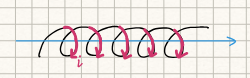
\includegraphics[width=6cm, height=2cm]{../img/soly.png}
\end{center}

\textit{Создаваемое магнитное поле будет направлено по оси соленоида.}

\vspace{5px}

Рассмотрим магнитное поле в других точках, будем считать что соленоид бесконечен:
\begin{enumerate}
    \item Возьмем два витка соленоида и рассмотрим такой рисунок
          \begin{center}
              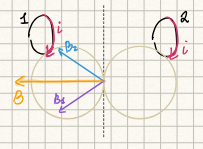
\includegraphics[width=6cm, height=4cm]{../img/soly_1.png}
          \end{center}
          \[|B_1| = |B_2| , \alpha = \beta \Rightarrow \vec B = \vec B_1 + \vec B_2\]
          \begin{center}
              где B || оси соленоида.
          \end{center}

    \item Возьмем замкнутый контур внутри соленоида
          \begin{center}
              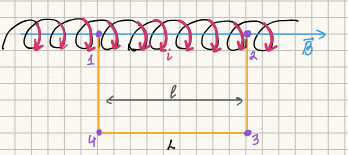
\includegraphics[width=9cm, height=4cm]{../img/soly_2.png}
          \end{center}
          \[ \oint_{\zeta} \vec B d \vec l = \int_{1,2} \vec B d \vec l + \int_{2,3} \vec B d \vec l + \int_{3,4} \vec B d \vec l + \int_{4,1} \vec B d \vec l\]

          \vspace{5px}

          Поскольку $\vec B \bot d \vec l \Rightarrow \int_{2,3} \vec B d \vec l = 0$ и $\int_{4,1} \vec B d \vec l = 0$,
          и при отдалении участка 3,4 от соленоида на бесконечности $\int_{3,4} \vec B d \vec l \to 0$ ,
          тогда:

          \[\oint_{\zeta} \vec B d \vec l = \int_{1,2} \vec B d \vec l \Rightarrow\]
          \begin{center}
              Из того что $\vec B \uparrow \uparrow \vec l \Rightarrow cos{\alpha} = 1$
          \end{center}
          \[B\int_{1,2} dl = Bl\]

    \item Пусть n - количество витков соленоида, приходящиея на единицу длины(n - плотность намотки).

          Тогда по теореме о циркуляции вектора $\vec B$:
          \[\oint_{\zeta} \vec B d \vec l = \mu_0 n i l\]
          Откуда
          \[B = \mu_0 n i\]
          \begin{center}
              --- внутри соленоида соответственно, вне соленоида $B = 0$
          \end{center}
          Во всех точках внутри соленоида поле будет одинаковым.
\end{enumerate}

\subsection{Магнитное поле в веществе}
Попадая в магнитное поле любое вещество приобретает магнитный момент(намагничивается) и создает вокруг себя собственное магнитное поле.

Пусть внешнее магнитное поле - $B_0$, а $\vec B^{\prime}$ - внутренне магнитное поле, тогда общее магнитное поле соотвественно:
\[\vec B = \vec B_0 + \vec B^{\prime}\]

Молекулярный ток:
\[P_m = i_m \cdot S\]
\begin{center}
    где $i_m$ - сила тока молекулы, $S$ - площадь контура вращения
\end{center}
Тогда вектор намагничивания:
\[\vec J = \frac{\sum_{\Delta V^{\prime}} \vec P_m}{\Delta V}\]

\subsection{Описание магнитного поля магнетика}
Возьмем замкнутую поверхность.

Очевидно. что $\oiint_{S} \vec B \vec n dS = 0$ поскольку линии замнуты, то есть при входе они обязательно выходят или \textit{количество линий входящих и выходящих одинаковое.}

Тогда с учетом $\vec B = \vec B_0 + \vec B^{\prime}$:
\[\oint_{\zeta} \vec B d \vec l = \oint_{\zeta} \vec B_0 d \vec l  + \oint_{\zeta} \vec B^{\prime} d \vec l = \mu_0 \sum i + \mu_0 \sum i_m \]

Возьмем маленький кусочек траектории $dl$, для упрощения будем считать, что все молекулярные точки имеют одинаковую площадь:
\begin{center}

    \definecolor{qqwuqq}{rgb}{0,0.39,0}
    \definecolor{wwqqff}{rgb}{0.4,0,1}
    \definecolor{qqccqq}{rgb}{0,0.8,0}
    \definecolor{qqqqff}{rgb}{0,0,1}
    \definecolor{fftttt}{rgb}{1,0.2,0.2}
    \definecolor{ttfftt}{rgb}{0.2,1,0.2}
    \begin{tikzpicture}[line cap=round,line join=round,>=triangle 45,x=1.3828442246291806cm,y=1.4011913919436727cm]
        \clip(13.14,68.48) rectangle (18.37,70.97);
        \fill[color=ttfftt,fill=ttfftt,fill opacity=0.1] (6.25,4.5) -- (7.72,6.84) -- (6.26,7.01) -- cycle;
        \draw [shift={(6.25,4.5)},color=fftttt,fill=fftttt,fill opacity=0.1] (0,0) -- (57.75:0.36) arc (57.75:89.85:0.36) -- cycle;
        \draw [shift={(14,23)},color=qqccqq,fill=qqccqq,fill opacity=0.1] (0,0) -- (-129.81:0.32) arc (-129.81:-90:0.32) -- cycle;
        \draw [shift={(9,17)},color=qqccqq,fill=qqccqq,fill opacity=0.1] (0,0) -- (50.19:0.36) arc (50.19:90:0.36) -- cycle;
        \draw [shift={(14,23)},color=wwqqff,fill=wwqqff,fill opacity=0.1] (0,0) -- (-149.04:0.24) arc (-149.04:-129.81:0.24) -- cycle;
        \draw [shift={(14.01,44.36)},color=qqwuqq,fill=qqwuqq,fill opacity=0.1] (0,0) -- (117.44:0.24) arc (117.44:180.25:0.24) -- cycle;
        \draw [shift={(14.91,59.59)},color=qqccqq,fill=qqccqq,fill opacity=0.1] (0,0) -- (-47.84:0.24) arc (-47.84:-3.25:0.24) -- cycle;
        \draw [shift={(13.5,58.5)},color=qqqqff,fill=qqqqff,fill opacity=0.1] (0,0) -- (-0.48:0.24) arc (-0.48:37.66:0.24) -- cycle;
        \draw [shift={(14.25,69.48)},color=qqwuqq,fill=qqwuqq,fill opacity=0.1] (0,0) -- (10.7:0.24) arc (10.7:43.65:0.24) -- cycle;
        \draw [rotate around={0:(6.27,7.02)},dash pattern=on 1pt off 1pt] (6.27,7.02) ellipse (2.22cm and 0.59cm);
        \draw [dash pattern=on 1pt off 1pt] (6.26,8.01)-- (6.25,4.5);
        \draw [dash pattern=on 1pt off 1pt] (6.25,4.5)-- (7.72,6.84);
        \draw [dash pattern=on 1pt off 1pt] (7.72,6.84)-- (6.26,7.01);
        \draw [->] (6.25,4.5) -- (6.25,5.48);
        \draw [->] (7.72,6.84) -- (8.23,7.21);
        \draw [dash pattern=on 1pt off 1pt,color=ttfftt] (6.25,4.5)-- (7.72,6.84);
        \draw [dash pattern=on 1pt off 1pt,color=ttfftt] (7.72,6.84)-- (6.26,7.01);
        \draw [dash pattern=on 1pt off 1pt,color=ttfftt] (6.26,7.01)-- (6.25,4.5);
        \draw [shift={(7.03,5.86)}] plot[domain=2.82:4.19,variable=\t]({1*1.57*cos(\t r)+0*1.57*sin(\t r)},{0*1.57*cos(\t r)+1*1.57*sin(\t r)});
        \draw [shift={(4.62,6.44)}] plot[domain=-0.09:1.62,variable=\t]({1*0.93*cos(\t r)+0*0.93*sin(\t r)},{0*0.93*cos(\t r)+1*0.93*sin(\t r)});
        \draw (4.57,7.36)-- (4.7,7.31);
        \draw (4.57,7.36)-- (4.71,7.42);
        \draw (7.91,7.15) node[anchor=north west] {$d \vec B$};
        \draw (4.8,7.75) node[anchor=north west] {$i$};
        \draw (5.86,5.37) node[anchor=north west] {$d \vec l$};
        \draw (6.97,5.65) node[anchor=north west] {$\vec r$};
        \draw [->] (6.25,4.5) -- (7.23,6.06);
        \draw (7.72,6.79) node[anchor=north west] {$A$};
        \draw [->] (9,17) -- (9,24);
        \draw [->] (9,17) -- (9,20);
        \draw (9,17)-- (14,23);
        \draw [->,color=qqqqff] (11,23) -- (9,23);
        \draw [->,color=qqqqff] (11,23) -- (14,23);
        \draw [dash pattern=on 1pt off 1pt] (14,23)-- (9,20);
        \draw (14,23)-- (14,17);
        \draw (9,20)-- (10.67,19);
        \draw [shift={(14,23)},color=wwqqff] (-149.04:0.24) arc (-149.04:-129.81:0.24);
        \draw [shift={(14,23)},color=wwqqff] (-149.04:0.2) arc (-149.04:-129.81:0.2);
        \draw [shift={(14,23)},color=wwqqff] (-149.04:0.16) arc (-149.04:-129.81:0.16);
        \draw [color=qqqqff](10.9,22.89) node[anchor=north west] {$b$};
        \draw (8.48,23.8) node[anchor=north west] {$i$};
        \draw (8.5,18.88) node[anchor=north west] {$d \vec l$};
        \draw [color=qqccqq](9.11,18.5) node[anchor=north west] {$\alpha$};
        \draw [color=qqccqq](13.45,22.46) node[anchor=north west] {$\alpha$};
        \draw (10.01,19.71) node[anchor=north west] {x};
        \draw [rotate around={-0.25:(11.95,44.33)}] (11.95,44.33) ellipse (2.85cm and 0.96cm);
        \draw [->] (11.84,44.35) -- (11.86,46.01);
        \draw [->] (14.01,44.36) -- (13.86,44.99);
        \draw (11.84,44.35)-- (14.01,44.36);
        \draw (11.84,44.35)-- (10.5,44.83);
        \draw (11.17,44.88) node[anchor=north west] {$R$};
        \draw (12.74,44.43) node[anchor=north west] {$\vec r$};
        \draw (13.06,43.78)-- (13.2,43.79);
        \draw (13.2,43.79)-- (13.08,43.73);
        \draw (12.94,43.98) node[anchor=north west] {$i$};
        \draw (13.95,44.85) node[anchor=north west] {$d \vec l$};
        \draw (11.92,45.44) node[anchor=north west] {$\vec B $};
        \draw [shift={(13.08,58.42)}] plot[domain=1.65:4.15,variable=\t]({1*1.09*cos(\t r)+0*1.09*sin(\t r)},{0*1.09*cos(\t r)+1*1.09*sin(\t r)});
        \draw [shift={(13.06,54.8)}] plot[domain=0.76:1.77,variable=\t]({1*2.76*cos(\t r)+0*2.76*sin(\t r)},{0*2.76*cos(\t r)+1*2.76*sin(\t r)});
        \draw [shift={(13.93,58.36)}] plot[domain=-0.97:0.27,variable=\t]({1*2*cos(\t r)+0*2*sin(\t r)},{0*2*cos(\t r)+1*2*sin(\t r)});
        \draw [shift={(14.06,57.45)}] plot[domain=0.67:2.05,variable=\t]({1*2.31*cos(\t r)+0*2.31*sin(\t r)},{0*2.31*cos(\t r)+1*2.31*sin(\t r)});
        \draw [->] (14.91,59.59) -- (13.5,58.5);
        \draw [->,color=qqccqq] (14.91,59.59) -- (16.5,59.5);
        \draw [->] (14.91,59.59) -- (16.23,58.13);
        \draw [color=qqccqq](15.3,60.03) node[anchor=north west] {$d \vec l$};
        \draw (13.72,59.31) node[anchor=north west] {$\vec r$};
        \draw (15.9,59.15) node[anchor=north west] {$\vec B$};
        \draw [dash pattern=on 1pt off 1pt] (13.5,58.5)-- (15.92,58.48);
        \draw (14.83,59.05) node[anchor=north west] {$dl_B$};
        \draw [rotate around={-55.56:(14.27,69.53)},dash pattern=on 1pt off 1pt] (14.27,69.53) ellipse (0.65cm and 0.46cm);
        \draw [rotate around={-64.94:(17.28,70.06)},dash pattern=on 1pt off 1pt] (17.28,70.06) ellipse (0.62cm and 0.42cm);
        \draw [dash pattern=on 1pt off 1pt] (14.07,69.95)-- (17.13,70.48);
        \draw [dash pattern=on 1pt off 1pt] (14.4,69.1)-- (17.4,69.63);
        \draw (14.25,69.48)-- (17.28,70.05);
        \draw [->] (14.25,69.48) -- (15.46,70.63);
        \draw (14.72,70.45) node[anchor=north west] {$\vec B$};
        \draw (15.78,69.78) node[anchor=north west] {$dl$};
        \begin{scriptsize}
            \draw[color=fftttt] (12.55,71.65) node {$\alpha$};
        \end{scriptsize}
    \end{tikzpicture}

\end{center}

Объем цилиндра: $dV_l = S_m \cdot dl \cdot cos{\alpha}$.

В самом цилиндре лежат центры молекул.

Обозначим за $n$ - концентрация, число молекул в единицу объема.

Тогда количество токов:
\[N_l = n \cdot dV_l = n \cdot S_m \cdot dl \cdot cos{\alpha}\]
Тогда:
\[\sum_{dl}i_m = n \cdot S_m \cdot dl \cdot cos{\alpha} \cdot i_m\]
С другой стороны:
\[S_m \cdot i_m = P_m\]
\begin{center}
    где $P_m \cdot n \cdot dl \cdot cos{\alpha}$ - модуль вектора намагниченности в проекци на $dl$
\end{center}
Тогда:
\[\sum_{dl} i_m = J \cdot dl \cdot cos{\alpha} = \vec J \cdot d \vec l \Rightarrow \sum i_m = \oint_{\zeta} \vec J \cdot d \vec l\]
Таким образм:
\[\oint_{\zeta} \vec B d \vec l = \mu_0 \sum i + \mu_0 \oint_{\zeta} \vec J \cdot d \vec l\]
Тогда:
\[\int_{\zeta}(\frac{\vec B}{\mu_0} - \vec J) d \vec l = \sum i\]

Вводится вспомагательная величина:
\[\vec H = \frac{\vec B}{\mu_0} - \vec J\]
\begin{center}
    --- \textit{\textbf{напряженность магнитного поля.}}

    Важно отметить, что $\vec H$ не учитывает молекулярные токи, поэтому $\vec H = \vec H_0$ - напряженность магнитного поля в вакууме.
\end{center}

\textit{\textbf{Теорема о циркуляции напряженности магнитного поля:}}
\[\oint_{\zeta} \vec H d \vec l = \sum i\]

Экспериментально было показано, что $\vec J = \chi \cdot \vec H \Rightarrow$:
\[\vec H(1+ \chi) = \frac{\vec B}{\mu_0} \Rightarrow \vec H = \frac{B}{\mu \mu_0}\]

Так $\chi$ может быть меньше 0 $\Rightarrow \mu $ может быть меньше единицы.

У некоторых веществ $\chi \neq const (\Rightarrow \mu \neq const )$ она зависит от магнитного поля.
В вакууме $\chi = 0, \mu = 1$.

Покажем, что $\vec H = \vec H_0$. Возьмем некоторый стержень и расположим его вдоль вектора магнитной индукции $\vec B_0$. Все молекулярные токи $i_m$ будут соориентированы перпендикулярно $\vec B$.

Заметим, что \textit{внутри} стрежня молекулярные токи $i_m$ компенсируются, а те которые вышли на границу ничем не компенсируются. Получается, что по контуру
циркулирует ток $I_1$, так как $I_1$ есть на протяжении всего стержня, то логично рассматривать его как соленоид.

\vspace{5px}

Выделим в соленоиде кусочек длины $dl$, посчитаем магнитный момент:
\[dp_m = S \cdot I_1 dl \Rightarrow dp_m = I_1 \cdot dv \Rightarrow \vec J = I_1 = \frac{dp_m}{dv}\]
\begin{center}
    --- это и есть вектор намагничивания $J$
\end{center}
Так подставим этот вектор $I_1 = J$, получим $\vec B^{\prime} = \mu_0 \cdot \vec J$, таким образом
\[\vec B = \vec B_0 + \vec B^{\prime} = \vec B_0 + \mu_0 \cdot \vec J\]
Из определения $\vec H = \frac{\vec B}{\mu_0} - \vec J$ :

\[\vec H = \frac{\vec B_0 + \mu_0 \cdot \vec J }{\mu_0} - \vec J\]
\[\vec H = \frac{\vec B_0}{\mu_0} = \vec H_0 \Rightarrow H = H_0\]

Таким образом. мы получили что $H$ в магнетике и в вакууме $H_0$ совпадают.

Отсюда вытекает:

\[
    \left\{
    \begin{aligned}
        \vec H   & = \frac{\vec B}{\mu \mu_0} \\
        \vec H_0 & = \frac{\vec B}{\mu_0}
    \end{aligned}
    \right.
    \quad \Rightarrow \quad
    \frac{B}{\mu} = B_0 \Rightarrow B = \mu \cdot B_0
\]
\begin{center}
    --- то есть $ \mu$ показывает во сколько раз изменяется магнитное поле в магнетике.
\end{center}

\textit{\textbf{Замечание:} Если магнитное поле расположено под углом, то так же как и электричске поле оно преломляется на границах.}
\subsection{Виды магнетиков}

\textit{\textbf{Классификация магнетиков}}
\begin{enumerate}
    \item Диамагнетики ($\chi < 0$, с порядком $10^{-8} \ldots 10^{-7}$)
    \item Парамагнетики ($\chi > 0$, с порядком $10^{-7} \ldots 10^{-4}$)
    \item Ферромагнетики ($\chi > 0$, с порядком $10^{3}$)
    \item Ферримагнетики
    \item Антиферромагнетики
\end{enumerate}
\begin{center}

    \definecolor{qqwuqq}{rgb}{0,0.39,0}
    \definecolor{wwqqff}{rgb}{0.4,0,1}
    \definecolor{qqccqq}{rgb}{0,0.8,0}
    \definecolor{qqqqff}{rgb}{0,0,1}
    \definecolor{fftttt}{rgb}{1,0.2,0.2}
    \definecolor{ttfftt}{rgb}{0.2,1,0.2}
    \begin{tikzpicture}[line cap=round,line join=round,>=triangle 45,x=4.437720328015432cm,y=5.287039467877825cm]
        \clip(17.15,83.57) rectangle (18.61,84.04);
        \fill[color=ttfftt,fill=ttfftt,fill opacity=0.1] (6.25,4.5) -- (7.72,6.84) -- (6.26,7.01) -- cycle;
        \draw [shift={(6.25,4.5)},color=fftttt,fill=fftttt,fill opacity=0.1] (0,0) -- (57.75:0.1) arc (57.75:89.85:0.1) -- cycle;
        \draw [shift={(14,23)},color=qqccqq,fill=qqccqq,fill opacity=0.1] (0,0) -- (-129.81:0.09) arc (-129.81:-90:0.09) -- cycle;
        \draw [shift={(9,17)},color=qqccqq,fill=qqccqq,fill opacity=0.1] (0,0) -- (50.19:0.1) arc (50.19:90:0.1) -- cycle;
        \draw [shift={(14,23)},color=wwqqff,fill=wwqqff,fill opacity=0.1] (0,0) -- (-149.04:0.07) arc (-149.04:-129.81:0.07) -- cycle;
        \draw [shift={(14.01,44.36)},color=qqwuqq,fill=qqwuqq,fill opacity=0.1] (0,0) -- (117.44:0.07) arc (117.44:180.25:0.07) -- cycle;
        \draw [shift={(14.91,59.59)},color=qqccqq,fill=qqccqq,fill opacity=0.1] (0,0) -- (-47.84:0.07) arc (-47.84:-3.25:0.07) -- cycle;
        \draw [shift={(13.5,58.5)},color=qqqqff,fill=qqqqff,fill opacity=0.1] (0,0) -- (-0.48:0.07) arc (-0.48:37.66:0.07) -- cycle;
        \draw [shift={(14.25,69.48)},color=qqwuqq,fill=qqwuqq,fill opacity=0.1] (0,0) -- (10.7:0.07) arc (10.7:43.65:0.07) -- cycle;
        \draw [rotate around={0:(6.27,7.02)},dash pattern=on 1pt off 1pt] (6.27,7.02) ellipse (7.12cm and 2.22cm);
        \draw [dash pattern=on 1pt off 1pt] (6.26,8.01)-- (6.25,4.5);
        \draw [dash pattern=on 1pt off 1pt] (6.25,4.5)-- (7.72,6.84);
        \draw [dash pattern=on 1pt off 1pt] (7.72,6.84)-- (6.26,7.01);
        \draw [->] (6.25,4.5) -- (6.25,5.48);
        \draw [->] (7.72,6.84) -- (8.23,7.21);
        \draw [dash pattern=on 1pt off 1pt,color=ttfftt] (6.25,4.5)-- (7.72,6.84);
        \draw [dash pattern=on 1pt off 1pt,color=ttfftt] (7.72,6.84)-- (6.26,7.01);
        \draw [dash pattern=on 1pt off 1pt,color=ttfftt] (6.26,7.01)-- (6.25,4.5);
        \draw [shift={(7.03,5.86)}] plot[domain=2.82:4.19,variable=\t]({1*1.57*cos(\t r)+0*1.57*sin(\t r)},{0*1.57*cos(\t r)+1*1.57*sin(\t r)});
        \draw [shift={(4.62,6.44)}] plot[domain=-0.09:1.62,variable=\t]({1*0.93*cos(\t r)+0*0.93*sin(\t r)},{0*0.93*cos(\t r)+1*0.93*sin(\t r)});
        \draw (4.57,7.36)-- (4.7,7.31);
        \draw (4.57,7.36)-- (4.71,7.42);
        \draw (7.91,7.08) node[anchor=north west] {$d \vec B$};
        \draw (4.8,7.68) node[anchor=north west] {$i$};
        \draw (5.87,5.31) node[anchor=north west] {$d \vec l$};
        \draw (6.97,5.59) node[anchor=north west] {$\vec r$};
        \draw [->] (6.25,4.5) -- (7.23,6.06);
        \draw (7.72,6.83) node[anchor=north west] {$A$};
        \draw [->] (9,17) -- (9,24);
        \draw [->] (9,17) -- (9,20);
        \draw (9,17)-- (14,23);
        \draw [->,color=qqqqff] (11,23) -- (9,23);
        \draw [->,color=qqqqff] (11,23) -- (14,23);
        \draw [dash pattern=on 1pt off 1pt] (14,23)-- (9,20);
        \draw (14,23)-- (14,17);
        \draw (9,20)-- (10.67,19);
        \draw [shift={(14,23)},color=wwqqff] (-149.04:0.07) arc (-149.04:-129.81:0.07);
        \draw [shift={(14,23)},color=wwqqff] (-149.04:0.06) arc (-149.04:-129.81:0.06);
        \draw [shift={(14,23)},color=wwqqff] (-149.04:0.05) arc (-149.04:-129.81:0.05);
        \draw [color=qqqqff](10.91,22.82) node[anchor=north west] {$b$};
        \draw (8.48,23.74) node[anchor=north west] {$i$};
        \draw (8.5,18.81) node[anchor=north west] {$d \vec l$};
        \draw [color=qqccqq](9.12,18.43) node[anchor=north west] {$\alpha$};
        \draw [color=qqccqq](13.45,22.38) node[anchor=north west] {$\alpha$};
        \draw (10,19.64) node[anchor=north west] {x};
        \draw [rotate around={-0.25:(11.95,44.33)}] (11.95,44.33) ellipse (9.15cm and 3.62cm);
        \draw [->] (11.84,44.35) -- (11.86,46.01);
        \draw [->] (14.01,44.36) -- (13.86,44.99);
        \draw (11.84,44.35)-- (14.01,44.36);
        \draw (11.84,44.35)-- (10.5,44.83);
        \draw (11.17,44.81) node[anchor=north west] {$R$};
        \draw (12.75,44.36) node[anchor=north west] {$\vec r$};
        \draw (13.06,43.78)-- (13.2,43.79);
        \draw (13.2,43.79)-- (13.08,43.73);
        \draw (12.93,43.91) node[anchor=north west] {$i$};
        \draw (13.94,44.78) node[anchor=north west] {$d \vec l$};
        \draw (11.92,45.37) node[anchor=north west] {$\vec B $};
        \draw [shift={(13.08,58.42)}] plot[domain=1.65:4.15,variable=\t]({1*1.09*cos(\t r)+0*1.09*sin(\t r)},{0*1.09*cos(\t r)+1*1.09*sin(\t r)});
        \draw [shift={(13.06,54.8)}] plot[domain=0.76:1.77,variable=\t]({1*2.76*cos(\t r)+0*2.76*sin(\t r)},{0*2.76*cos(\t r)+1*2.76*sin(\t r)});
        \draw [shift={(13.93,58.36)}] plot[domain=-0.97:0.27,variable=\t]({1*2*cos(\t r)+0*2*sin(\t r)},{0*2*cos(\t r)+1*2*sin(\t r)});
        \draw [shift={(14.06,57.45)}] plot[domain=0.67:2.05,variable=\t]({1*2.31*cos(\t r)+0*2.31*sin(\t r)},{0*2.31*cos(\t r)+1*2.31*sin(\t r)});
        \draw [->] (14.91,59.59) -- (13.5,58.5);
        \draw [->,color=qqccqq] (14.91,59.59) -- (16.5,59.5);
        \draw [->] (14.91,59.59) -- (16.23,58.13);
        \draw [color=qqccqq](15.3,59.96) node[anchor=north west] {$d \vec l$};
        \draw (13.72,59.24) node[anchor=north west] {$\vec r$};
        \draw (15.9,59.08) node[anchor=north west] {$\vec B$};
        \draw [dash pattern=on 1pt off 1pt] (13.5,58.5)-- (15.92,58.48);
        \draw (14.83,58.98) node[anchor=north west] {$dl_B$};
        \draw [rotate around={-55.56:(14.27,69.53)},dash pattern=on 1pt off 1pt] (14.27,69.53) ellipse (2.09cm and 1.73cm);
        \draw [rotate around={-64.94:(17.28,70.06)},dash pattern=on 1pt off 1pt] (17.28,70.06) ellipse (2cm and 1.58cm);
        \draw [dash pattern=on 1pt off 1pt] (14.07,69.95)-- (17.13,70.48);
        \draw [dash pattern=on 1pt off 1pt] (14.4,69.1)-- (17.4,69.63);
        \draw (14.25,69.48)-- (17.28,70.05);
        \draw [->] (14.25,69.48) -- (15.46,70.63);
        \draw (14.72,70.38) node[anchor=north west] {$\vec B$};
        \draw (15.78,69.71) node[anchor=north west] {$dl$};
        \draw [->] (17.2,83.8) -- (18.6,83.8);
        \draw(17.8,83.8) ellipse (0.89cm and 1.06cm);
        \draw (17.94,83.97)-- (17.95,83.93);
        \draw (17.95,83.93)-- (17.91,83.94);
        \draw (18.44,83.9) node[anchor=north west] {$\vec B$};
        \begin{scriptsize}
            \draw[color=fftttt] (16.97,84.44) node {$\alpha$};
        \end{scriptsize}
    \end{tikzpicture}

\end{center}
Электрон вращается вокруг ядра по некоторой окружности. Значит он обладает орбитальным моментом $p_m$. Но электрон также обладает собственным магнитным моментом --- спином($p_s$).
Складываяясь они влияют на магнитный момент молекулы.
\begin{itemize}
    \item Собственный магнитный момент есть у всех магнетиков за исключением диамагнетиков, то есть $p_s, p_m$ скомпенсировали друг друга. Диамагнетики намагничиваются против направления магнитного поля.

          --- \textit{\textbf{Явление диамагнетизма}} : происходит прецессия орбиты электрона, то есть она сама начинает вращаться. Это создает дополнительное смещение электрона.

    \item  У парамагнетиков все молекулы обладают магнитным моментом, но они перемешаны и в магнитном поле разворачиваются,
          создавая намагниченность, то есть без магнитного поля они друг друга компенсируют.

    \item Ферромагнетики обладают доменной структурой, то есть в некоторых локальнх областях магнитные моменты направлены в одну сторону. То ест всне магнитного поля они также
          не намагничиваются, но в магнитном поле они все стремятся развернутся в одну сторону, значительно усиливая магнитное поле.
          После снятия магнитного поля намагниченность ферромагнетиков уменьшается, но сохраняется, то есть обладают остаточной намагниченностью.У ферромагнетиков имеется точка Кюри. Магнетик
          перестает быть ферромагнетиком и становится парамагнетиком.
          \begin{center}

              \definecolor{qqwuqq}{rgb}{0,0.39,0}
              \definecolor{wwqqff}{rgb}{0.4,0,1}
              \definecolor{qqccqq}{rgb}{0,0.8,0}
              \definecolor{qqqqff}{rgb}{0,0,1}
              \definecolor{fftttt}{rgb}{1,0.2,0.2}
              \definecolor{ttfftt}{rgb}{0.2,1,0.2}
              \begin{tikzpicture}[line cap=round,line join=round,>=triangle 45,x=1.0cm,y=1.0cm]
                  \clip(7.59,90.95) rectangle (17.8,95.07);
                  \fill[color=ttfftt,fill=ttfftt,fill opacity=0.1] (6.25,4.5) -- (7.72,6.84) -- (6.26,7.01) -- cycle;
                  \draw [shift={(6.25,4.5)},color=fftttt,fill=fftttt,fill opacity=0.1] (0,0) -- (57.75:0.72) arc (57.75:89.85:0.72) -- cycle;
                  \draw [shift={(14,23)},color=qqccqq,fill=qqccqq,fill opacity=0.1] (0,0) -- (-129.81:0.64) arc (-129.81:-90:0.64) -- cycle;
                  \draw [shift={(9,17)},color=qqccqq,fill=qqccqq,fill opacity=0.1] (0,0) -- (50.19:0.72) arc (50.19:90:0.72) -- cycle;
                  \draw [shift={(14,23)},color=wwqqff,fill=wwqqff,fill opacity=0.1] (0,0) -- (-149.04:0.48) arc (-149.04:-129.81:0.48) -- cycle;
                  \draw [shift={(14.01,44.36)},color=qqwuqq,fill=qqwuqq,fill opacity=0.1] (0,0) -- (117.44:0.48) arc (117.44:180.25:0.48) -- cycle;
                  \draw [shift={(14.91,59.59)},color=qqccqq,fill=qqccqq,fill opacity=0.1] (0,0) -- (-47.84:0.48) arc (-47.84:-3.25:0.48) -- cycle;
                  \draw [shift={(13.5,58.5)},color=qqqqff,fill=qqqqff,fill opacity=0.1] (0,0) -- (-0.48:0.48) arc (-0.48:37.66:0.48) -- cycle;
                  \draw [shift={(14.25,69.48)},color=qqwuqq,fill=qqwuqq,fill opacity=0.1] (0,0) -- (10.7:0.48) arc (10.7:43.65:0.48) -- cycle;
                  \draw [rotate around={0:(6.27,7.02)},dash pattern=on 1pt off 1pt] (6.27,7.02) ellipse (1.6cm and 0.42cm);
                  \draw [dash pattern=on 1pt off 1pt] (6.26,8.01)-- (6.25,4.5);
                  \draw [dash pattern=on 1pt off 1pt] (6.25,4.5)-- (7.72,6.84);
                  \draw [dash pattern=on 1pt off 1pt] (7.72,6.84)-- (6.26,7.01);
                  \draw [->] (6.25,4.5) -- (6.25,5.48);
                  \draw [->] (7.72,6.84) -- (8.23,7.21);
                  \draw [dash pattern=on 1pt off 1pt,color=ttfftt] (6.25,4.5)-- (7.72,6.84);
                  \draw [dash pattern=on 1pt off 1pt,color=ttfftt] (7.72,6.84)-- (6.26,7.01);
                  \draw [dash pattern=on 1pt off 1pt,color=ttfftt] (6.26,7.01)-- (6.25,4.5);
                  \draw [shift={(7.03,5.86)}] plot[domain=2.82:4.19,variable=\t]({1*1.57*cos(\t r)+0*1.57*sin(\t r)},{0*1.57*cos(\t r)+1*1.57*sin(\t r)});
                  \draw [shift={(4.62,6.44)}] plot[domain=-0.09:1.62,variable=\t]({1*0.93*cos(\t r)+0*0.93*sin(\t r)},{0*0.93*cos(\t r)+1*0.93*sin(\t r)});
                  \draw (4.57,7.36)-- (4.7,7.31);
                  \draw (4.57,7.36)-- (4.71,7.42);
                  \draw (7.92,7.25) node[anchor=north west] {$d \vec B$};
                  \draw (4.8,7.84) node[anchor=north west] {$i$};
                  \draw (5.87,5.47) node[anchor=north west] {$d \vec l$};
                  \draw (6.97,5.75) node[anchor=north west] {$\vec r$};
                  \draw [->] (6.25,4.5) -- (7.23,6.06);
                  \draw (7.71,6.74) node[anchor=north west] {$A$};
                  \draw [->] (9,17) -- (9,24);
                  \draw [->] (9,17) -- (9,20);
                  \draw (9,17)-- (14,23);
                  \draw [->,color=qqqqff] (11,23) -- (9,23);
                  \draw [->,color=qqqqff] (11,23) -- (14,23);
                  \draw [dash pattern=on 1pt off 1pt] (14,23)-- (9,20);
                  \draw (14,23)-- (14,17);
                  \draw (9,20)-- (10.67,19);
                  \draw [shift={(14,23)},color=wwqqff] (-149.04:0.48) arc (-149.04:-129.81:0.48);
                  \draw [shift={(14,23)},color=wwqqff] (-149.04:0.4) arc (-149.04:-129.81:0.4);
                  \draw [shift={(14,23)},color=wwqqff] (-149.04:0.32) arc (-149.04:-129.81:0.32);
                  \draw [color=qqqqff](10.91,22.99) node[anchor=north west] {$b$};
                  \draw (8.48,23.89) node[anchor=north west] {$i$};
                  \draw (8.49,18.98) node[anchor=north west] {$d \vec l$};
                  \draw [color=qqccqq](9.11,18.59) node[anchor=north west] {$\alpha$};
                  \draw [color=qqccqq](13.44,22.54) node[anchor=north west] {$\alpha$};
                  \draw (10,19.8) node[anchor=north west] {x};
                  \draw [rotate around={-0.25:(11.95,44.33)}] (11.95,44.33) ellipse (2.06cm and 0.68cm);
                  \draw [->] (11.84,44.35) -- (11.86,46.01);
                  \draw [->] (14.01,44.36) -- (13.86,44.99);
                  \draw (11.84,44.35)-- (14.01,44.36);
                  \draw (11.84,44.35)-- (10.5,44.83);
                  \draw (11.17,44.98) node[anchor=north west] {$R$};
                  \draw (12.74,44.52) node[anchor=north west] {$\vec r$};
                  \draw (13.06,43.78)-- (13.2,43.79);
                  \draw (13.2,43.79)-- (13.08,43.73);
                  \draw (12.93,44.07) node[anchor=north west] {$i$};
                  \draw (13.95,44.95) node[anchor=north west] {$d \vec l$};
                  \draw (11.91,45.53) node[anchor=north west] {$\vec B $};
                  \draw [shift={(13.08,58.42)}] plot[domain=1.65:4.15,variable=\t]({1*1.09*cos(\t r)+0*1.09*sin(\t r)},{0*1.09*cos(\t r)+1*1.09*sin(\t r)});
                  \draw [shift={(13.06,54.8)}] plot[domain=0.76:1.77,variable=\t]({1*2.76*cos(\t r)+0*2.76*sin(\t r)},{0*2.76*cos(\t r)+1*2.76*sin(\t r)});
                  \draw [shift={(13.93,58.36)}] plot[domain=-0.97:0.27,variable=\t]({1*2*cos(\t r)+0*2*sin(\t r)},{0*2*cos(\t r)+1*2*sin(\t r)});
                  \draw [shift={(14.06,57.45)}] plot[domain=0.67:2.05,variable=\t]({1*2.31*cos(\t r)+0*2.31*sin(\t r)},{0*2.31*cos(\t r)+1*2.31*sin(\t r)});
                  \draw [->] (14.91,59.59) -- (13.5,58.5);
                  \draw [->,color=qqccqq] (14.91,59.59) -- (16.5,59.5);
                  \draw [->] (14.91,59.59) -- (16.23,58.13);
                  \draw [color=qqccqq](15.3,60.13) node[anchor=north west] {$d \vec l$};
                  \draw (13.71,59.41) node[anchor=north west] {$\vec r$};
                  \draw (15.89,59.25) node[anchor=north west] {$\vec B$};
                  \draw [dash pattern=on 1pt off 1pt] (13.5,58.5)-- (15.92,58.48);
                  \draw (14.83,59.14) node[anchor=north west] {$dl_B$};
                  \draw [rotate around={-55.56:(14.27,69.53)},dash pattern=on 1pt off 1pt] (14.27,69.53) ellipse (0.47cm and 0.33cm);
                  \draw [rotate around={-64.94:(17.28,70.06)},dash pattern=on 1pt off 1pt] (17.28,70.06) ellipse (0.45cm and 0.3cm);
                  \draw [dash pattern=on 1pt off 1pt] (14.07,69.95)-- (17.13,70.48);
                  \draw [dash pattern=on 1pt off 1pt] (14.4,69.1)-- (17.4,69.63);
                  \draw (14.25,69.48)-- (17.28,70.05);
                  \draw [->] (14.25,69.48) -- (15.46,70.63);
                  \draw (14.71,70.55) node[anchor=north west] {$\vec B$};
                  \draw (15.78,69.88) node[anchor=north west] {$dl$};
                  \draw [->] (17.2,83.8) -- (18.6,83.8);
                  \draw(17.8,83.8) circle (0.2cm);
                  \draw (17.94,83.97)-- (17.95,83.93);
                  \draw (17.95,83.93)-- (17.91,83.94);
                  \draw (18.44,84.06) node[anchor=north west] {$\vec B$};
                  \draw (8,94)-- (8,92);
                  \draw (8,92)-- (12,92);
                  \draw (12,92)-- (12,94);
                  \draw (12,94)-- (8,94);
                  \draw (13,94)-- (17,94);
                  \draw (17,92)-- (13,92);
                  \draw (13,94)-- (13,92);
                  \draw (17,94)-- (17,92);
                  \draw [shift={(8.13,94.91)}] plot[domain=4.64:5.79,variable=\t]({1*1.92*cos(\t r)+0*1.92*sin(\t r)},{0*1.92*cos(\t r)+1*1.92*sin(\t r)});
                  \draw [shift={(8.27,92.89)}] plot[domain=-0.71:0.5,variable=\t]({1*1.37*cos(\t r)+0*1.37*sin(\t r)},{0*1.37*cos(\t r)+1*1.37*sin(\t r)});
                  \draw [shift={(11.01,88.83)}] plot[domain=1.31:1.95,variable=\t]({1*3.91*cos(\t r)+0*3.91*sin(\t r)},{0*3.91*cos(\t r)+1*3.91*sin(\t r)});
                  \draw [shift={(11.75,93.81)}] plot[domain=2.95:4.07,variable=\t]({1*1.34*cos(\t r)+0*1.34*sin(\t r)},{0*1.34*cos(\t r)+1*1.34*sin(\t r)});
                  \draw (13,94)-- (13,92);
                  \draw (13,92)-- (17,92);
                  \draw (17,92)-- (17,94);
                  \draw (17,94)-- (13,94);
                  \draw [shift={(13.13,94.91)}] plot[domain=4.64:5.79,variable=\t]({1*1.92*cos(\t r)+0*1.92*sin(\t r)},{0*1.92*cos(\t r)+1*1.92*sin(\t r)});
                  \draw [shift={(13.27,92.89)}] plot[domain=-0.71:0.5,variable=\t]({1*1.37*cos(\t r)+0*1.37*sin(\t r)},{0*1.37*cos(\t r)+1*1.37*sin(\t r)});
                  \draw [shift={(16.01,88.83)}] plot[domain=1.31:1.95,variable=\t]({1*3.91*cos(\t r)+0*3.91*sin(\t r)},{0*3.91*cos(\t r)+1*3.91*sin(\t r)});
                  \draw [shift={(16.75,93.81)}] plot[domain=2.95:4.07,variable=\t]({1*1.34*cos(\t r)+0*1.34*sin(\t r)},{0*1.34*cos(\t r)+1*1.34*sin(\t r)});
                  \draw [->] (8.68,93.26) -- (8.24,93.7);
                  \draw [->] (9,93.53) -- (8.62,93.89);
                  \draw [->] (8.46,92.58) -- (9,92);
                  \draw [->] (8.87,92.75) -- (9.27,92.29);
                  \draw [->] (9.98,93.51) -- (10.01,92.8);
                  \draw [->] (10.2,93.51) -- (10.28,92.8);
                  \draw [->] (10.28,92.15) -- (11.04,92.48);
                  \draw [->] (10.89,92.15) -- (11.57,92.36);
                  \draw [->] (11.26,93.56) -- (11.61,92.96);
                  \draw [->] (11.57,93.7) -- (11.88,93.15);
                  \draw [->] (13.28,93.73) -- (14.18,93.75);
                  \draw [->] (13.17,93.45) -- (14.07,93.46);
                  \draw [->] (13.46,92.78) -- (14.36,92.8);
                  \draw [->] (13.44,92.44) -- (14.34,92.45);
                  \draw [->] (15.12,92.4) -- (16.02,92.42);
                  \draw [->] (15.12,92.17) -- (16.02,92.18);
                  \draw [->] (15.84,93.72) -- (16.75,93.73);
                  \draw [->] (15.89,93.42) -- (16.79,93.43);
                  \draw [->] (14.71,93.21) -- (15.33,93.22);
                  \draw [->] (14.75,92.91) -- (15.65,92.92);
                  \draw [->] (13,94.48) -- (17.01,94.46);
                  \draw (16.51,95.1) node[anchor=north west] {$B_0$};
                  \draw (9.27,92.05) node[anchor=north west] {$\vec B_0 = 0$};
                  \draw (14.6,92.01) node[anchor=north west] {$\vec B_0 \neq 0$};
                  \begin{scriptsize}
                      \draw[color=fftttt] (7.52,99.3) node {$\alpha$};
                  \end{scriptsize}
              \end{tikzpicture}

          \end{center}

    \item Ферримагнетики состоят из двух слоев --- из более намагниченного внешнего слоя и слабо намагниченного внутреннего слоя, направленного противоположно внешнему слою.
          \begin{center}

              \definecolor{qqwuqq}{rgb}{0,0.39,0}
              \definecolor{wwqqff}{rgb}{0.4,0,1}
              \definecolor{qqccqq}{rgb}{0,0.8,0}
              \definecolor{qqqqff}{rgb}{0,0,1}
              \definecolor{fftttt}{rgb}{1,0.2,0.2}
              \definecolor{ttfftt}{rgb}{0.2,1,0.2}
              \begin{tikzpicture}[line cap=round,line join=round,>=triangle 45,x=1.0cm,y=1.0cm]
                  \clip(12.47,111.74) rectangle (26.06,118.5);
                  \fill[color=ttfftt,fill=ttfftt,fill opacity=0.1] (6.25,4.5) -- (7.72,6.84) -- (6.26,7.01) -- cycle;
                  \draw [shift={(6.25,4.5)},color=fftttt,fill=fftttt,fill opacity=0.1] (0,0) -- (57.75:0.78) arc (57.75:89.85:0.78) -- cycle;
                  \draw [shift={(14,23)},color=qqccqq,fill=qqccqq,fill opacity=0.1] (0,0) -- (-129.81:0.7) arc (-129.81:-90:0.7) -- cycle;
                  \draw [shift={(9,17)},color=qqccqq,fill=qqccqq,fill opacity=0.1] (0,0) -- (50.19:0.78) arc (50.19:90:0.78) -- cycle;
                  \draw [shift={(14,23)},color=wwqqff,fill=wwqqff,fill opacity=0.1] (0,0) -- (-149.04:0.52) arc (-149.04:-129.81:0.52) -- cycle;
                  \draw [shift={(14.01,44.36)},color=qqwuqq,fill=qqwuqq,fill opacity=0.1] (0,0) -- (117.44:0.52) arc (117.44:180.25:0.52) -- cycle;
                  \draw [shift={(14.91,59.59)},color=qqccqq,fill=qqccqq,fill opacity=0.1] (0,0) -- (-47.84:0.52) arc (-47.84:-3.25:0.52) -- cycle;
                  \draw [shift={(13.5,58.5)},color=qqqqff,fill=qqqqff,fill opacity=0.1] (0,0) -- (-0.48:0.52) arc (-0.48:37.66:0.52) -- cycle;
                  \draw [shift={(14.25,69.48)},color=qqwuqq,fill=qqwuqq,fill opacity=0.1] (0,0) -- (10.7:0.52) arc (10.7:43.65:0.52) -- cycle;
                  \draw [rotate around={0:(6.27,7.02)},dash pattern=on 1pt off 1pt] (6.27,7.02) ellipse (1.6cm and 0.42cm);
                  \draw [dash pattern=on 1pt off 1pt] (6.26,8.01)-- (6.25,4.5);
                  \draw [dash pattern=on 1pt off 1pt] (6.25,4.5)-- (7.72,6.84);
                  \draw [dash pattern=on 1pt off 1pt] (7.72,6.84)-- (6.26,7.01);
                  \draw [->] (6.25,4.5) -- (6.25,5.48);
                  \draw [->] (7.72,6.84) -- (8.23,7.21);
                  \draw [dash pattern=on 1pt off 1pt,color=ttfftt] (6.25,4.5)-- (7.72,6.84);
                  \draw [dash pattern=on 1pt off 1pt,color=ttfftt] (7.72,6.84)-- (6.26,7.01);
                  \draw [dash pattern=on 1pt off 1pt,color=ttfftt] (6.26,7.01)-- (6.25,4.5);
                  \draw [shift={(7.03,5.86)}] plot[domain=2.82:4.19,variable=\t]({1*1.57*cos(\t r)+0*1.57*sin(\t r)},{0*1.57*cos(\t r)+1*1.57*sin(\t r)});
                  \draw [shift={(4.62,6.44)}] plot[domain=-0.09:1.62,variable=\t]({1*0.93*cos(\t r)+0*0.93*sin(\t r)},{0*0.93*cos(\t r)+1*0.93*sin(\t r)});
                  \draw (4.57,7.36)-- (4.7,7.31);
                  \draw (4.57,7.36)-- (4.71,7.42);
                  \draw (7.91,7.26) node[anchor=north west] {$d \vec B$};
                  \draw (4.79,7.87) node[anchor=north west] {$i$};
                  \draw (5.87,5.5) node[anchor=north west] {$d \vec l$};
                  \draw (6.97,5.76) node[anchor=north west] {$\vec r$};
                  \draw [->] (6.25,4.5) -- (7.23,6.06);
                  \draw (7.7,6.74) node[anchor=north west] {$A$};
                  \draw [->] (9,17) -- (9,24);
                  \draw [->] (9,17) -- (9,20);
                  \draw (9,17)-- (14,23);
                  \draw [->,color=qqqqff] (11,23) -- (9,23);
                  \draw [->,color=qqqqff] (11,23) -- (14,23);
                  \draw [dash pattern=on 1pt off 1pt] (14,23)-- (9,20);
                  \draw (14,23)-- (14,17);
                  \draw (9,20)-- (10.67,19);
                  \draw [shift={(14,23)},color=wwqqff] (-149.04:0.52) arc (-149.04:-129.81:0.52);
                  \draw [shift={(14,23)},color=wwqqff] (-149.04:0.44) arc (-149.04:-129.81:0.44);
                  \draw [shift={(14,23)},color=wwqqff] (-149.04:0.35) arc (-149.04:-129.81:0.35);
                  \draw [color=qqqqff](10.9,23.01) node[anchor=north west] {$b$};
                  \draw (8.48,23.91) node[anchor=north west] {$i$};
                  \draw (8.5,18.98) node[anchor=north west] {$d \vec l$};
                  \draw [color=qqccqq](9.11,18.62) node[anchor=north west] {$\alpha$};
                  \draw [color=qqccqq](13.45,22.57) node[anchor=north west] {$\alpha$};
                  \draw (10,19.82) node[anchor=north west] {x};
                  \draw [rotate around={-0.25:(11.95,44.33)}] (11.95,44.33) ellipse (2.06cm and 0.68cm);
                  \draw [->] (11.84,44.35) -- (11.86,46.01);
                  \draw [->] (14.01,44.36) -- (13.86,44.99);
                  \draw (11.84,44.35)-- (14.01,44.36);
                  \draw (11.84,44.35)-- (10.5,44.83);
                  \draw (11.17,44.99) node[anchor=north west] {$R$};
                  \draw (12.75,44.54) node[anchor=north west] {$\vec r$};
                  \draw (13.06,43.78)-- (13.2,43.79);
                  \draw (13.2,43.79)-- (13.08,43.73);
                  \draw (12.93,44.09) node[anchor=north west] {$i$};
                  \draw (13.94,44.96) node[anchor=north west] {$d \vec l$};
                  \draw (11.92,45.55) node[anchor=north west] {$\vec B $};
                  \draw [shift={(13.08,58.42)}] plot[domain=1.65:4.15,variable=\t]({1*1.09*cos(\t r)+0*1.09*sin(\t r)},{0*1.09*cos(\t r)+1*1.09*sin(\t r)});
                  \draw [shift={(13.06,54.8)}] plot[domain=0.76:1.77,variable=\t]({1*2.76*cos(\t r)+0*2.76*sin(\t r)},{0*2.76*cos(\t r)+1*2.76*sin(\t r)});
                  \draw [shift={(13.93,58.36)}] plot[domain=-0.97:0.27,variable=\t]({1*2*cos(\t r)+0*2*sin(\t r)},{0*2*cos(\t r)+1*2*sin(\t r)});
                  \draw [shift={(14.06,57.45)}] plot[domain=0.67:2.05,variable=\t]({1*2.31*cos(\t r)+0*2.31*sin(\t r)},{0*2.31*cos(\t r)+1*2.31*sin(\t r)});
                  \draw [->] (14.91,59.59) -- (13.5,58.5);
                  \draw [->,color=qqccqq] (14.91,59.59) -- (16.5,59.5);
                  \draw [->] (14.91,59.59) -- (16.23,58.13);
                  \draw [color=qqccqq](15.29,60.13) node[anchor=north west] {$d \vec l$};
                  \draw (13.71,59.42) node[anchor=north west] {$\vec r$};
                  \draw (15.9,59.26) node[anchor=north west] {$\vec B$};
                  \draw [dash pattern=on 1pt off 1pt] (13.5,58.5)-- (15.92,58.48);
                  \draw (14.82,59.16) node[anchor=north west] {$dl_B$};
                  \draw [rotate around={-55.56:(14.27,69.53)},dash pattern=on 1pt off 1pt] (14.27,69.53) ellipse (0.47cm and 0.33cm);
                  \draw [rotate around={-64.94:(17.28,70.06)},dash pattern=on 1pt off 1pt] (17.28,70.06) ellipse (0.45cm and 0.3cm);
                  \draw [dash pattern=on 1pt off 1pt] (14.07,69.95)-- (17.13,70.48);
                  \draw [dash pattern=on 1pt off 1pt] (14.4,69.1)-- (17.4,69.63);
                  \draw (14.25,69.48)-- (17.28,70.05);
                  \draw [->] (14.25,69.48) -- (15.46,70.63);
                  \draw (14.72,70.57) node[anchor=north west] {$\vec B$};
                  \draw (15.78,69.89) node[anchor=north west] {$dl$};
                  \draw [->] (17.2,83.8) -- (18.6,83.8);
                  \draw(17.8,83.8) circle (0.2cm);
                  \draw (17.94,83.97)-- (17.95,83.93);
                  \draw (17.95,83.93)-- (17.91,83.94);
                  \draw (18.43,84.09) node[anchor=north west] {$\vec B$};
                  \draw (8,94)-- (8,92);
                  \draw (8,92)-- (12,92);
                  \draw (12,92)-- (12,94);
                  \draw (12,94)-- (8,94);
                  \draw (13,94)-- (17,94);
                  \draw (17,92)-- (13,92);
                  \draw (13,94)-- (13,92);
                  \draw (17,94)-- (17,92);
                  \draw [shift={(8.13,94.91)}] plot[domain=4.64:5.79,variable=\t]({1*1.92*cos(\t r)+0*1.92*sin(\t r)},{0*1.92*cos(\t r)+1*1.92*sin(\t r)});
                  \draw [shift={(8.27,92.89)}] plot[domain=-0.71:0.5,variable=\t]({1*1.37*cos(\t r)+0*1.37*sin(\t r)},{0*1.37*cos(\t r)+1*1.37*sin(\t r)});
                  \draw [shift={(11.01,88.83)}] plot[domain=1.31:1.95,variable=\t]({1*3.91*cos(\t r)+0*3.91*sin(\t r)},{0*3.91*cos(\t r)+1*3.91*sin(\t r)});
                  \draw [shift={(11.75,93.81)}] plot[domain=2.95:4.07,variable=\t]({1*1.34*cos(\t r)+0*1.34*sin(\t r)},{0*1.34*cos(\t r)+1*1.34*sin(\t r)});
                  \draw (13,94)-- (13,92);
                  \draw (13,92)-- (17,92);
                  \draw (17,92)-- (17,94);
                  \draw (17,94)-- (13,94);
                  \draw [shift={(13.13,94.91)}] plot[domain=4.64:5.79,variable=\t]({1*1.92*cos(\t r)+0*1.92*sin(\t r)},{0*1.92*cos(\t r)+1*1.92*sin(\t r)});
                  \draw [shift={(13.27,92.89)}] plot[domain=-0.71:0.5,variable=\t]({1*1.37*cos(\t r)+0*1.37*sin(\t r)},{0*1.37*cos(\t r)+1*1.37*sin(\t r)});
                  \draw [shift={(16.01,88.83)}] plot[domain=1.31:1.95,variable=\t]({1*3.91*cos(\t r)+0*3.91*sin(\t r)},{0*3.91*cos(\t r)+1*3.91*sin(\t r)});
                  \draw [shift={(16.75,93.81)}] plot[domain=2.95:4.07,variable=\t]({1*1.34*cos(\t r)+0*1.34*sin(\t r)},{0*1.34*cos(\t r)+1*1.34*sin(\t r)});
                  \draw [->] (8.68,93.26) -- (8.24,93.7);
                  \draw [->] (9,93.53) -- (8.62,93.89);
                  \draw [->] (8.46,92.58) -- (9,92);
                  \draw [->] (8.87,92.75) -- (9.27,92.29);
                  \draw [->] (9.98,93.51) -- (10.01,92.8);
                  \draw [->] (10.2,93.51) -- (10.28,92.8);
                  \draw [->] (10.28,92.15) -- (11.04,92.48);
                  \draw [->] (10.89,92.15) -- (11.57,92.36);
                  \draw [->] (11.26,93.56) -- (11.61,92.96);
                  \draw [->] (11.57,93.7) -- (11.88,93.15);
                  \draw [->] (13.28,93.73) -- (14.18,93.75);
                  \draw [->] (13.17,93.45) -- (14.07,93.46);
                  \draw [->] (13.46,92.78) -- (14.36,92.8);
                  \draw [->] (13.44,92.44) -- (14.34,92.45);
                  \draw [->] (15.12,92.4) -- (16.02,92.42);
                  \draw [->] (15.12,92.17) -- (16.02,92.18);
                  \draw [->] (15.84,93.72) -- (16.75,93.73);
                  \draw [->] (15.89,93.42) -- (16.79,93.43);
                  \draw [->] (14.71,93.21) -- (15.33,93.22);
                  \draw [->] (14.75,92.91) -- (15.65,92.92);
                  \draw [->] (13,94.48) -- (17.01,94.46);
                  \draw (16.51,95.12) node[anchor=north west] {$B_0$};
                  \draw (9.28,92.07) node[anchor=north west] {$\vec B_0 = 0$};
                  \draw (14.6,92.03) node[anchor=north west] {$\vec B_0 \neq 0$};
                  \draw [line width=1.2pt] (13,117)-- (13,113);
                  \draw [line width=1.2pt] (17,113)-- (19,114);
                  \draw [line width=1.2pt] (19,114)-- (19,118);
                  \draw [line width=1.2pt] (19,118)-- (17,117);
                  \draw [line width=1.2pt] (17,117)-- (17,113);
                  \draw [line width=1.2pt] (13,117)-- (17,117);
                  \draw [line width=1.2pt] (13,113)-- (17,113);
                  \draw [line width=1.2pt] (13,117)-- (15,118);
                  \draw [line width=1.2pt] (19,118)-- (15,118);
                  \draw (13,113)-- (15,114);
                  \draw [dash pattern=on 1pt off 1pt] (15,118)-- (15,114);
                  \draw [dash pattern=on 1pt off 1pt] (15,114)-- (19,114);
                  \draw [color=qqccqq] (14.5,116)-- (15.28,116.37);
                  \draw [line width=1.2pt,color=qqccqq] (14.5,116)-- (14.5,114.5);
                  \draw [line width=1.2pt,color=qqccqq] (14.5,114.5)-- (16,114.5);
                  \draw [line width=1.2pt,color=qqccqq] (14.5,116)-- (16,116);
                  \draw [line width=1.2pt,color=qqccqq] (16,116)-- (16,114.5);
                  \draw [color=qqccqq] (16,116)-- (16.67,116.36);
                  \draw [color=qqccqq] (15.28,116.37)-- (16.67,116.36);
                  \draw [color=qqccqq] (15.28,116.37)-- (15.25,114.86);
                  \draw (14.5,114.5)-- (15.25,114.86);
                  \draw [color=qqccqq] (16.67,116.36)-- (16.66,114.86);
                  \draw [color=qqccqq] (16,114.5)-- (16.66,114.86);
                  \draw (16.66,114.86)-- (15.25,114.86);
                  \draw [color=qqccqq] (14.5,114.5)-- (13,113);
                  \draw [color=qqccqq] (14.5,116)-- (13,117);
                  \draw [dash pattern=on 1pt off 1pt,color=qqccqq] (15.28,116.37)-- (15,118);
                  \draw [color=qqccqq] (16,114.5)-- (17,113);
                  \draw [dash pattern=on 1pt off 1pt,color=qqccqq] (16.66,114.86)-- (19,114);
                  \draw [dash pattern=on 1pt off 1pt,color=qqccqq] (16.67,116.36)-- (19,118);
                  \draw [color=qqccqq] (16,116)-- (17,117);
                  \draw [dash pattern=on 1pt off 1pt,color=qqccqq] (15.25,114.86)-- (15,114);
                  \draw (20,117)-- (25,117);
                  \draw (20,115)-- (25,115);
                  \draw (25,117)-- (25,115);
                  \draw (20,117)-- (20,115);
                  \draw (21,117)-- (21,115);
                  \draw (22,117)-- (22,115);
                  \draw (23,117)-- (23,115);
                  \draw (24,117)-- (24,115);
                  \draw [->] (20.5,115.5) -- (20.5,116.65);
                  \draw [->] (22.51,115.52) -- (22.49,116.72);
                  \draw [->] (24.58,115.49) -- (24.56,116.76);
                  \draw [->,color=qqccqq] (21.44,116.2) -- (21.44,115.4);
                  \draw [->,color=qqccqq] (23.55,116.16) -- (23.59,115.42);
                  \begin{scriptsize}
                      \draw[color=fftttt] (11.98,120.82) node {$\alpha$};
                  \end{scriptsize}
              \end{tikzpicture}

          \end{center}

          Таким образом, они обладают разными по модулю магнитными моментами.

          Ферримагнетики могут быть диэлектриком и полупроводником.

    \item Антиферромагнетики также обладают доменной структурой, но их соседние молекулы противоположно направлены. При изменении внешнего магнитного поля изменяется сопротивление антиферромагнетика.
\end{itemize}

\subsection{Действие магнитного поля на токи и заряды}

Возьмем элемент проводника с током $dl$, на него соответственно действует сила $df$
\[d \vec f = ki \cdot [d \vec l, \vec B]\]

Тогда сила, действующая на единицу длины проводника:
\[d \vec f = i \cdot [d \vec l, \vec B]\]
\begin{center}
    --- \textit{\textbf{Закон Ампера}}
\end{center}
\subsubsection{Сила Лоренца}

Скажем, что $i = j \cdot S$, тогда
\[d \vec F = S \cdot dl \cdot [\vec j, \vec B] \Rightarrow\]
\begin{center}
    где $d \vec l$ и $ \vec j$ направлены в одну сторону
\end{center}
\[d \vec f = dV \cdot [\vec j, \vec B] \langle \text{в силу} \vec j = q \cdot n \cdot V \rangle \Rightarrow \]
\[d \vec f = q \cdot [\vec V, \vec B] n \cdot dV \Rightarrow \frac{df}{dN} = F_l = q[\vec V, \vec B]\]

Сила с которой магнитное поле действует на движущуюся заряженную частицу:
\[F_l = q[\vec V, \vec B]\]
\begin{center}
    --- \textit{\textbf{Сила Лоренца}}
\end{center}

где $\vec B$ - индукция магнитного поля, $\vec V$ - скорость частицы.

\subsection{Контур с током в магнитном поле}
Пусть имеется некоторый контур с током, направленным изначально вниз:
\begin{center}

    \definecolor{qqwuqq}{rgb}{0,0.39,0}
    \definecolor{wwqqff}{rgb}{0.4,0,1}
    \definecolor{qqccqq}{rgb}{0,0.8,0}
    \definecolor{qqqqff}{rgb}{0,0,1}
    \definecolor{fftttt}{rgb}{1,0.2,0.2}
    \definecolor{ttfftt}{rgb}{0.2,1,0.2}
    \begin{tikzpicture}[line cap=round,line join=round,>=triangle 45,x=1.0cm,y=1.0cm]
        \clip(23.95,149.63) rectangle (34.15,156.83);
        \fill[color=ttfftt,fill=ttfftt,fill opacity=0.1] (6.25,4.5) -- (7.72,6.84) -- (6.26,7.01) -- cycle;
        \draw [shift={(6.25,4.5)},color=fftttt,fill=fftttt,fill opacity=0.1] (0,0) -- (57.75:0.78) arc (57.75:89.85:0.78) -- cycle;
        \draw [shift={(14,23)},color=qqccqq,fill=qqccqq,fill opacity=0.1] (0,0) -- (-129.81:0.7) arc (-129.81:-90:0.7) -- cycle;
        \draw [shift={(9,17)},color=qqccqq,fill=qqccqq,fill opacity=0.1] (0,0) -- (50.19:0.78) arc (50.19:90:0.78) -- cycle;
        \draw [shift={(14,23)},color=wwqqff,fill=wwqqff,fill opacity=0.1] (0,0) -- (-149.04:0.52) arc (-149.04:-129.81:0.52) -- cycle;
        \draw [shift={(14.01,44.36)},color=qqwuqq,fill=qqwuqq,fill opacity=0.1] (0,0) -- (117.44:0.52) arc (117.44:180.25:0.52) -- cycle;
        \draw [shift={(14.91,59.59)},color=qqccqq,fill=qqccqq,fill opacity=0.1] (0,0) -- (-47.84:0.52) arc (-47.84:-3.25:0.52) -- cycle;
        \draw [shift={(13.5,58.5)},color=qqqqff,fill=qqqqff,fill opacity=0.1] (0,0) -- (-0.48:0.52) arc (-0.48:37.66:0.52) -- cycle;
        \draw [shift={(14.25,69.48)},color=qqwuqq,fill=qqwuqq,fill opacity=0.1] (0,0) -- (10.7:0.52) arc (10.7:43.65:0.52) -- cycle;
        \draw [shift={(25,153)},color=qqwuqq,fill=qqwuqq,fill opacity=0.1] (0,0) -- (45:0.52) arc (45:90:0.52) -- cycle;
        \draw [shift={(33,154)},color=qqwuqq,fill=qqwuqq,fill opacity=0.1] (0,0) -- (-135:0.52) arc (-135:-90:0.52) -- cycle;
        \draw [rotate around={0:(6.27,7.02)},dash pattern=on 1pt off 1pt] (6.27,7.02) ellipse (1.6cm and 0.42cm);
        \draw [dash pattern=on 1pt off 1pt] (6.26,8.01)-- (6.25,4.5);
        \draw [dash pattern=on 1pt off 1pt] (6.25,4.5)-- (7.72,6.84);
        \draw [dash pattern=on 1pt off 1pt] (7.72,6.84)-- (6.26,7.01);
        \draw [->] (6.25,4.5) -- (6.25,5.48);
        \draw [->] (7.72,6.84) -- (8.23,7.21);
        \draw [dash pattern=on 1pt off 1pt,color=ttfftt] (6.25,4.5)-- (7.72,6.84);
        \draw [dash pattern=on 1pt off 1pt,color=ttfftt] (7.72,6.84)-- (6.26,7.01);
        \draw [dash pattern=on 1pt off 1pt,color=ttfftt] (6.26,7.01)-- (6.25,4.5);
        \draw [shift={(7.03,5.86)}] plot[domain=2.82:4.19,variable=\t]({1*1.57*cos(\t r)+0*1.57*sin(\t r)},{0*1.57*cos(\t r)+1*1.57*sin(\t r)});
        \draw [shift={(4.62,6.44)}] plot[domain=-0.09:1.62,variable=\t]({1*0.93*cos(\t r)+0*0.93*sin(\t r)},{0*0.93*cos(\t r)+1*0.93*sin(\t r)});
        \draw (4.57,7.36)-- (4.7,7.31);
        \draw (4.57,7.36)-- (4.71,7.42);
        \draw (7.91,7.26) node[anchor=north west] {$d \vec B$};
        \draw (4.79,7.87) node[anchor=north west] {$i$};
        \draw (5.87,5.5) node[anchor=north west] {$d \vec l$};
        \draw (6.97,5.76) node[anchor=north west] {$\vec r$};
        \draw [->] (6.25,4.5) -- (7.23,6.06);
        \draw (7.7,6.74) node[anchor=north west] {$A$};
        \draw [->] (9,17) -- (9,24);
        \draw [->] (9,17) -- (9,20);
        \draw (9,17)-- (14,23);
        \draw [->,color=qqqqff] (11,23) -- (9,23);
        \draw [->,color=qqqqff] (11,23) -- (14,23);
        \draw [dash pattern=on 1pt off 1pt] (14,23)-- (9,20);
        \draw (14,23)-- (14,17);
        \draw (9,20)-- (10.67,19);
        \draw [shift={(14,23)},color=wwqqff] (-149.04:0.52) arc (-149.04:-129.81:0.52);
        \draw [shift={(14,23)},color=wwqqff] (-149.04:0.44) arc (-149.04:-129.81:0.44);
        \draw [shift={(14,23)},color=wwqqff] (-149.04:0.35) arc (-149.04:-129.81:0.35);
        \draw [color=qqqqff](10.9,23.01) node[anchor=north west] {$b$};
        \draw (8.48,23.91) node[anchor=north west] {$i$};
        \draw (8.5,18.98) node[anchor=north west] {$d \vec l$};
        \draw [color=qqccqq](9.11,18.62) node[anchor=north west] {$\alpha$};
        \draw [color=qqccqq](13.45,22.57) node[anchor=north west] {$\alpha$};
        \draw (10,19.82) node[anchor=north west] {x};
        \draw [rotate around={-0.25:(11.95,44.33)}] (11.95,44.33) ellipse (2.06cm and 0.68cm);
        \draw [->] (11.84,44.35) -- (11.86,46.01);
        \draw [->] (14.01,44.36) -- (13.86,44.99);
        \draw (11.84,44.35)-- (14.01,44.36);
        \draw (11.84,44.35)-- (10.5,44.83);
        \draw (11.17,44.99) node[anchor=north west] {$R$};
        \draw (12.75,44.54) node[anchor=north west] {$\vec r$};
        \draw (13.06,43.78)-- (13.2,43.79);
        \draw (13.2,43.79)-- (13.08,43.73);
        \draw (12.93,44.09) node[anchor=north west] {$i$};
        \draw (13.94,44.96) node[anchor=north west] {$d \vec l$};
        \draw (11.92,45.55) node[anchor=north west] {$\vec B $};
        \draw [shift={(13.08,58.42)}] plot[domain=1.65:4.15,variable=\t]({1*1.09*cos(\t r)+0*1.09*sin(\t r)},{0*1.09*cos(\t r)+1*1.09*sin(\t r)});
        \draw [shift={(13.06,54.8)}] plot[domain=0.76:1.77,variable=\t]({1*2.76*cos(\t r)+0*2.76*sin(\t r)},{0*2.76*cos(\t r)+1*2.76*sin(\t r)});
        \draw [shift={(13.93,58.36)}] plot[domain=-0.97:0.27,variable=\t]({1*2*cos(\t r)+0*2*sin(\t r)},{0*2*cos(\t r)+1*2*sin(\t r)});
        \draw [shift={(14.06,57.45)}] plot[domain=0.67:2.05,variable=\t]({1*2.31*cos(\t r)+0*2.31*sin(\t r)},{0*2.31*cos(\t r)+1*2.31*sin(\t r)});
        \draw [->] (14.91,59.59) -- (13.5,58.5);
        \draw [->,color=qqccqq] (14.91,59.59) -- (16.5,59.5);
        \draw [->] (14.91,59.59) -- (16.23,58.13);
        \draw [color=qqccqq](15.29,60.13) node[anchor=north west] {$d \vec l$};
        \draw (13.71,59.42) node[anchor=north west] {$\vec r$};
        \draw (15.9,59.26) node[anchor=north west] {$\vec B$};
        \draw [dash pattern=on 1pt off 1pt] (13.5,58.5)-- (15.92,58.48);
        \draw (14.82,59.16) node[anchor=north west] {$dl_B$};
        \draw [rotate around={-55.56:(14.27,69.53)},dash pattern=on 1pt off 1pt] (14.27,69.53) ellipse (0.47cm and 0.33cm);
        \draw [rotate around={-64.94:(17.28,70.06)},dash pattern=on 1pt off 1pt] (17.28,70.06) ellipse (0.45cm and 0.3cm);
        \draw [dash pattern=on 1pt off 1pt] (14.07,69.95)-- (17.13,70.48);
        \draw [dash pattern=on 1pt off 1pt] (14.4,69.1)-- (17.4,69.63);
        \draw (14.25,69.48)-- (17.28,70.05);
        \draw [->] (14.25,69.48) -- (15.46,70.63);
        \draw (14.72,70.57) node[anchor=north west] {$\vec B$};
        \draw (15.78,69.89) node[anchor=north west] {$dl$};
        \draw [->] (17.2,83.8) -- (18.6,83.8);
        \draw(17.8,83.8) circle (0.2cm);
        \draw (17.94,83.97)-- (17.95,83.93);
        \draw (17.95,83.93)-- (17.91,83.94);
        \draw (18.43,84.09) node[anchor=north west] {$\vec B$};
        \draw (8,94)-- (8,92);
        \draw (8,92)-- (12,92);
        \draw (12,92)-- (12,94);
        \draw (12,94)-- (8,94);
        \draw (13,94)-- (17,94);
        \draw (17,92)-- (13,92);
        \draw (13,94)-- (13,92);
        \draw (17,94)-- (17,92);
        \draw [shift={(8.13,94.91)}] plot[domain=4.64:5.79,variable=\t]({1*1.92*cos(\t r)+0*1.92*sin(\t r)},{0*1.92*cos(\t r)+1*1.92*sin(\t r)});
        \draw [shift={(8.27,92.89)}] plot[domain=-0.71:0.5,variable=\t]({1*1.37*cos(\t r)+0*1.37*sin(\t r)},{0*1.37*cos(\t r)+1*1.37*sin(\t r)});
        \draw [shift={(11.01,88.83)}] plot[domain=1.31:1.95,variable=\t]({1*3.91*cos(\t r)+0*3.91*sin(\t r)},{0*3.91*cos(\t r)+1*3.91*sin(\t r)});
        \draw [shift={(11.75,93.81)}] plot[domain=2.95:4.07,variable=\t]({1*1.34*cos(\t r)+0*1.34*sin(\t r)},{0*1.34*cos(\t r)+1*1.34*sin(\t r)});
        \draw (13,94)-- (13,92);
        \draw (13,92)-- (17,92);
        \draw (17,92)-- (17,94);
        \draw (17,94)-- (13,94);
        \draw [shift={(13.13,94.91)}] plot[domain=4.64:5.79,variable=\t]({1*1.92*cos(\t r)+0*1.92*sin(\t r)},{0*1.92*cos(\t r)+1*1.92*sin(\t r)});
        \draw [shift={(13.27,92.89)}] plot[domain=-0.71:0.5,variable=\t]({1*1.37*cos(\t r)+0*1.37*sin(\t r)},{0*1.37*cos(\t r)+1*1.37*sin(\t r)});
        \draw [shift={(16.01,88.83)}] plot[domain=1.31:1.95,variable=\t]({1*3.91*cos(\t r)+0*3.91*sin(\t r)},{0*3.91*cos(\t r)+1*3.91*sin(\t r)});
        \draw [shift={(16.75,93.81)}] plot[domain=2.95:4.07,variable=\t]({1*1.34*cos(\t r)+0*1.34*sin(\t r)},{0*1.34*cos(\t r)+1*1.34*sin(\t r)});
        \draw [->] (8.68,93.26) -- (8.24,93.7);
        \draw [->] (9,93.53) -- (8.62,93.89);
        \draw [->] (8.46,92.58) -- (9,92);
        \draw [->] (8.87,92.75) -- (9.27,92.29);
        \draw [->] (9.98,93.51) -- (10.01,92.8);
        \draw [->] (10.2,93.51) -- (10.28,92.8);
        \draw [->] (10.28,92.15) -- (11.04,92.48);
        \draw [->] (10.89,92.15) -- (11.57,92.36);
        \draw [->] (11.26,93.56) -- (11.61,92.96);
        \draw [->] (11.57,93.7) -- (11.88,93.15);
        \draw [->] (13.28,93.73) -- (14.18,93.75);
        \draw [->] (13.17,93.45) -- (14.07,93.46);
        \draw [->] (13.46,92.78) -- (14.36,92.8);
        \draw [->] (13.44,92.44) -- (14.34,92.45);
        \draw [->] (15.12,92.4) -- (16.02,92.42);
        \draw [->] (15.12,92.17) -- (16.02,92.18);
        \draw [->] (15.84,93.72) -- (16.75,93.73);
        \draw [->] (15.89,93.42) -- (16.79,93.43);
        \draw [->] (14.71,93.21) -- (15.33,93.22);
        \draw [->] (14.75,92.91) -- (15.65,92.92);
        \draw [->] (13,94.48) -- (17.01,94.46);
        \draw (16.51,95.12) node[anchor=north west] {$B_0$};
        \draw (9.28,92.07) node[anchor=north west] {$\vec B_0 = 0$};
        \draw (14.6,92.03) node[anchor=north west] {$\vec B_0 \neq 0$};
        \draw [line width=1.2pt] (13,117)-- (13,113);
        \draw [line width=1.2pt] (17,113)-- (19,114);
        \draw [line width=1.2pt] (19,114)-- (19,118);
        \draw [line width=1.2pt] (19,118)-- (17,117);
        \draw [line width=1.2pt] (17,117)-- (17,113);
        \draw [line width=1.2pt] (13,117)-- (17,117);
        \draw [line width=1.2pt] (13,113)-- (17,113);
        \draw [line width=1.2pt] (13,117)-- (15,118);
        \draw [line width=1.2pt] (19,118)-- (15,118);
        \draw (13,113)-- (15,114);
        \draw [dash pattern=on 1pt off 1pt] (15,118)-- (15,114);
        \draw [dash pattern=on 1pt off 1pt] (15,114)-- (19,114);
        \draw [color=qqccqq] (14.5,116)-- (15.28,116.37);
        \draw [line width=1.2pt,color=qqccqq] (14.5,116)-- (14.5,114.5);
        \draw [line width=1.2pt,color=qqccqq] (14.5,114.5)-- (16,114.5);
        \draw [line width=1.2pt,color=qqccqq] (14.5,116)-- (16,116);
        \draw [line width=1.2pt,color=qqccqq] (16,116)-- (16,114.5);
        \draw [color=qqccqq] (16,116)-- (16.67,116.36);
        \draw [color=qqccqq] (15.28,116.37)-- (16.67,116.36);
        \draw [color=qqccqq] (15.28,116.37)-- (15.25,114.86);
        \draw (14.5,114.5)-- (15.25,114.86);
        \draw [color=qqccqq] (16.67,116.36)-- (16.66,114.86);
        \draw [color=qqccqq] (16,114.5)-- (16.66,114.86);
        \draw (16.66,114.86)-- (15.25,114.86);
        \draw [color=qqccqq] (14.5,114.5)-- (13,113);
        \draw [color=qqccqq] (14.5,116)-- (13,117);
        \draw [dash pattern=on 1pt off 1pt,color=qqccqq] (15.28,116.37)-- (15,118);
        \draw [color=qqccqq] (16,114.5)-- (17,113);
        \draw [dash pattern=on 1pt off 1pt,color=qqccqq] (16.66,114.86)-- (19,114);
        \draw [dash pattern=on 1pt off 1pt,color=qqccqq] (16.67,116.36)-- (19,118);
        \draw [color=qqccqq] (16,116)-- (17,117);
        \draw [dash pattern=on 1pt off 1pt,color=qqccqq] (15.25,114.86)-- (15,114);
        \draw (20,117)-- (25,117);
        \draw (20,115)-- (25,115);
        \draw (25,117)-- (25,115);
        \draw (20,117)-- (20,115);
        \draw (21,117)-- (21,115);
        \draw (22,117)-- (22,115);
        \draw (23,117)-- (23,115);
        \draw (24,117)-- (24,115);
        \draw [->] (20.5,115.5) -- (20.5,116.65);
        \draw [->] (22.51,115.52) -- (22.49,116.72);
        \draw [->] (24.58,115.49) -- (24.56,116.76);
        \draw [->,color=qqccqq] (21.44,116.2) -- (21.44,115.4);
        \draw [->,color=qqccqq] (23.55,116.16) -- (23.59,115.42);
        \draw (25,156)-- (33,156);
        \draw (25,156)-- (25,151);
        \draw (33,156)-- (33,151);
        \draw (33,151)-- (25,151);
        \draw [dash pattern=on 1pt off 1pt] (29.01,156.46)-- (28.99,150.38);
        \draw [->] (25,150) -- (31,150);
        \draw [->] (32,151) -- (26,151);
        \draw [->] (33,155) -- (33,153);
        \draw [->] (27,156) -- (31,156);
        \draw [->] (25,153) -- (25,155);
        \draw (24.6,151.53) node[anchor=north west] {$1$};
        \draw (24.72,156.46) node[anchor=north west] {$2$};
        \draw (33.2,156.44) node[anchor=north west] {$3$};
        \draw (33.17,151.57) node[anchor=north west] {$4$};
        \draw (27.63,151.65) node[anchor=north west] {$b$};
        \draw [->,color=qqccqq] (25,153) -- (26,154);
        \draw [->,color=qqccqq] (33,154) -- (32,153);
        \draw [->,color=qqccqq] (33,151) -- (33,150);
        \draw [->,color=qqccqq] (25,151) -- (25,150);
        \draw (25.57,153.71) node[anchor=north west] {$\vec F_{1,2}$};
        \draw (31.78,154.18) node[anchor=north west] {$\vec F_{3,4}$};
        \draw (25.1,150.9) node[anchor=north west] {$M_{1,2}$};
        \draw (32.33,150.85) node[anchor=north west] {$M_{3,4}$};
        \draw (30.21,150.63) node[anchor=north west] {$\vec B$};
        \begin{scriptsize}
            \draw[color=fftttt] (22.7,157.79) node {$\alpha$};
        \end{scriptsize}
    \end{tikzpicture}

\end{center}
Используем закон Ампера:
\[F_{1,2} = i \cdot a \cdot b ; F_{3,4} = i \cdot a \cdot B\]
\[F_{2,3} = 0 ; F_{4,1} = 0\]
Силы стремятся повернуть контур вокруг оси, проходящей через центр:
\[M_{1,2} = F_{1,2} \cdot \frac{b}{2} ; M_{3,4} = F_{3,4} \cdot \frac{b}{2}\]
Тогда
\[M = M_{1,2} + M_{3,4} = i \cdot a \cdot b \cdot B = i \cdot S \cdot B = P_m \cdot B
    \Rightarrow B = \frac{M_{max}}{P_m}\]

\begin{center}

    \definecolor{qqwuqq}{rgb}{0,0.39,0}
    \definecolor{wwqqff}{rgb}{0.4,0,1}
    \definecolor{qqccqq}{rgb}{0,0.8,0}
    \definecolor{qqqqff}{rgb}{0,0,1}
    \definecolor{fftttt}{rgb}{1,0.2,0.2}
    \definecolor{ttfftt}{rgb}{0.2,1,0.2}
    \begin{tikzpicture}[line cap=round,line join=round,>=triangle 45,x=1.0cm,y=1.0cm]
        \clip(21.45,178.67) rectangle (36.92,184.28);
        \fill[color=ttfftt,fill=ttfftt,fill opacity=0.1] (6.25,4.5) -- (7.72,6.84) -- (6.26,7.01) -- cycle;
        \draw [shift={(6.25,4.5)},color=fftttt,fill=fftttt,fill opacity=0.1] (0,0) -- (57.75:0.69) arc (57.75:89.85:0.69) -- cycle;
        \draw [shift={(14,23)},color=qqccqq,fill=qqccqq,fill opacity=0.1] (0,0) -- (-129.81:0.61) arc (-129.81:-90:0.61) -- cycle;
        \draw [shift={(9,17)},color=qqccqq,fill=qqccqq,fill opacity=0.1] (0,0) -- (50.19:0.69) arc (50.19:90:0.69) -- cycle;
        \draw [shift={(14,23)},color=wwqqff,fill=wwqqff,fill opacity=0.1] (0,0) -- (-149.04:0.46) arc (-149.04:-129.81:0.46) -- cycle;
        \draw [shift={(14.01,44.36)},color=qqwuqq,fill=qqwuqq,fill opacity=0.1] (0,0) -- (117.44:0.46) arc (117.44:180.25:0.46) -- cycle;
        \draw [shift={(14.91,59.59)},color=qqccqq,fill=qqccqq,fill opacity=0.1] (0,0) -- (-47.84:0.46) arc (-47.84:-3.25:0.46) -- cycle;
        \draw [shift={(13.5,58.5)},color=qqqqff,fill=qqqqff,fill opacity=0.1] (0,0) -- (-0.48:0.46) arc (-0.48:37.66:0.46) -- cycle;
        \draw [shift={(14.25,69.48)},color=qqwuqq,fill=qqwuqq,fill opacity=0.1] (0,0) -- (10.7:0.46) arc (10.7:43.65:0.46) -- cycle;
        \draw [shift={(25,153)},color=qqwuqq,fill=qqwuqq,fill opacity=0.1] (0,0) -- (45:0.46) arc (45:90:0.46) -- cycle;
        \draw [shift={(33,154)},color=qqwuqq,fill=qqwuqq,fill opacity=0.1] (0,0) -- (-135:0.46) arc (-135:-90:0.46) -- cycle;
        \draw [rotate around={0:(6.27,7.02)},dash pattern=on 1pt off 1pt] (6.27,7.02) ellipse (1.6cm and 0.42cm);
        \draw [dash pattern=on 1pt off 1pt] (6.25,4.5)-- (7.72,6.84);
        \draw [dash pattern=on 1pt off 1pt] (7.72,6.84)-- (6.26,7.01);
        \draw [->] (6.25,4.5) -- (6.25,5.48);
        \draw [->] (7.72,6.84) -- (8.23,7.21);
        \draw [dash pattern=on 1pt off 1pt,color=ttfftt] (6.25,4.5)-- (7.72,6.84);
        \draw [dash pattern=on 1pt off 1pt,color=ttfftt] (7.72,6.84)-- (6.26,7.01);
        \draw [dash pattern=on 1pt off 1pt,color=ttfftt] (6.26,7.01)-- (6.25,4.5);
        \draw [shift={(7.03,5.86)}] plot[domain=2.82:4.19,variable=\t]({1*1.57*cos(\t r)+0*1.57*sin(\t r)},{0*1.57*cos(\t r)+1*1.57*sin(\t r)});
        \draw [shift={(4.62,6.44)}] plot[domain=-0.09:1.62,variable=\t]({1*0.93*cos(\t r)+0*0.93*sin(\t r)},{0*0.93*cos(\t r)+1*0.93*sin(\t r)});
        \draw (4.57,7.36)-- (4.7,7.31);
        \draw (4.57,7.36)-- (4.71,7.42);
        \draw (7.91,7.23) node[anchor=north west] {$d \vec B$};
        \draw (4.8,7.84) node[anchor=north west] {$i$};
        \draw (5.86,5.46) node[anchor=north west] {$d \vec l$};
        \draw (6.96,5.74) node[anchor=north west] {$\vec r$};
        \draw [->] (6.25,4.5) -- (7.23,6.06);
        \draw (7.71,6.74) node[anchor=north west] {$A$};
        \draw [->] (9,17) -- (9,24);
        \draw [->] (9,17) -- (9,20);
        \draw (9,17)-- (14,23);
        \draw [->,color=qqqqff] (11,23) -- (9,23);
        \draw [->,color=qqqqff] (11,23) -- (14,23);
        \draw [dash pattern=on 1pt off 1pt] (14,23)-- (9,20);
        \draw (14,23)-- (14,17);
        \draw (9,20)-- (10.67,19);
        \draw [shift={(14,23)},color=wwqqff] (-149.04:0.46) arc (-149.04:-129.81:0.46);
        \draw [shift={(14,23)},color=wwqqff] (-149.04:0.38) arc (-149.04:-129.81:0.38);
        \draw [shift={(14,23)},color=wwqqff] (-149.04:0.31) arc (-149.04:-129.81:0.31);
        \draw [color=qqqqff](10.91,22.97) node[anchor=north west] {$b$};
        \draw (8.49,23.89) node[anchor=north west] {$i$};
        \draw (8.5,18.96) node[anchor=north west] {$d \vec l$};
        \draw [color=qqccqq](9.11,18.58) node[anchor=north west] {$\alpha$};
        \draw [color=qqccqq](13.44,22.54) node[anchor=north west] {$\alpha$};
        \draw (10,19.8) node[anchor=north west] {x};
        \draw [rotate around={-0.25:(11.95,44.33)}] (11.95,44.33) ellipse (2.06cm and 0.68cm);
        \draw [->] (11.84,44.35) -- (11.86,46.01);
        \draw [->] (14.01,44.36) -- (13.86,44.99);
        \draw (11.84,44.35)-- (14.01,44.36);
        \draw (11.84,44.35)-- (10.5,44.83);
        \draw (11.17,44.97) node[anchor=north west] {$R$};
        \draw (12.74,44.51) node[anchor=north west] {$\vec r$};
        \draw (13.06,43.78)-- (13.2,43.79);
        \draw (13.2,43.79)-- (13.08,43.73);
        \draw (12.93,44.07) node[anchor=north west] {$i$};
        \draw (13.95,44.94) node[anchor=north west] {$d \vec l$};
        \draw (11.92,45.53) node[anchor=north west] {$\vec B $};
        \draw [shift={(13.08,58.42)}] plot[domain=1.65:4.15,variable=\t]({1*1.09*cos(\t r)+0*1.09*sin(\t r)},{0*1.09*cos(\t r)+1*1.09*sin(\t r)});
        \draw [shift={(13.06,54.8)}] plot[domain=0.76:1.77,variable=\t]({1*2.76*cos(\t r)+0*2.76*sin(\t r)},{0*2.76*cos(\t r)+1*2.76*sin(\t r)});
        \draw [shift={(13.93,58.36)}] plot[domain=-0.97:0.27,variable=\t]({1*2*cos(\t r)+0*2*sin(\t r)},{0*2*cos(\t r)+1*2*sin(\t r)});
        \draw [shift={(14.06,57.45)}] plot[domain=0.67:2.05,variable=\t]({1*2.31*cos(\t r)+0*2.31*sin(\t r)},{0*2.31*cos(\t r)+1*2.31*sin(\t r)});
        \draw [->] (14.91,59.59) -- (13.5,58.5);
        \draw [->,color=qqccqq] (14.91,59.59) -- (16.5,59.5);
        \draw [->] (14.91,59.59) -- (16.23,58.13);
        \draw [color=qqccqq](15.31,60.11) node[anchor=north west] {$d \vec l$};
        \draw (13.72,59.39) node[anchor=north west] {$\vec r$};
        \draw (15.9,59.24) node[anchor=north west] {$\vec B$};
        \draw [dash pattern=on 1pt off 1pt] (13.5,58.5)-- (15.92,58.48);
        \draw (14.83,59.14) node[anchor=north west] {$dl_B$};
        \draw [rotate around={-55.56:(14.27,69.53)},dash pattern=on 1pt off 1pt] (14.27,69.53) ellipse (0.47cm and 0.33cm);
        \draw [rotate around={-64.94:(17.28,70.06)},dash pattern=on 1pt off 1pt] (17.28,70.06) ellipse (0.45cm and 0.3cm);
        \draw [dash pattern=on 1pt off 1pt] (14.07,69.95)-- (17.13,70.48);
        \draw [dash pattern=on 1pt off 1pt] (14.4,69.1)-- (17.4,69.63);
        \draw (14.25,69.48)-- (17.28,70.05);
        \draw [->] (14.25,69.48) -- (15.46,70.63);
        \draw (14.73,70.54) node[anchor=north west] {$\vec B$};
        \draw (15.78,69.87) node[anchor=north west] {$dl$};
        \draw [->] (17.2,83.8) -- (18.6,83.8);
        \draw(17.8,83.8) circle (0.2cm);
        \draw (17.94,83.97)-- (17.95,83.93);
        \draw (17.95,83.93)-- (17.91,83.94);
        \draw (18.43,84.06) node[anchor=north west] {$\vec B$};
        \draw (8,94)-- (8,92);
        \draw (8,92)-- (12,92);
        \draw (12,92)-- (12,94);
        \draw (12,94)-- (8,94);
        \draw (13,94)-- (17,94);
        \draw (17,92)-- (13,92);
        \draw (13,94)-- (13,92);
        \draw (17,94)-- (17,92);
        \draw [shift={(8.13,94.91)}] plot[domain=4.64:5.79,variable=\t]({1*1.92*cos(\t r)+0*1.92*sin(\t r)},{0*1.92*cos(\t r)+1*1.92*sin(\t r)});
        \draw [shift={(8.27,92.89)}] plot[domain=-0.71:0.5,variable=\t]({1*1.37*cos(\t r)+0*1.37*sin(\t r)},{0*1.37*cos(\t r)+1*1.37*sin(\t r)});
        \draw [shift={(11.01,88.83)}] plot[domain=1.31:1.95,variable=\t]({1*3.91*cos(\t r)+0*3.91*sin(\t r)},{0*3.91*cos(\t r)+1*3.91*sin(\t r)});
        \draw [shift={(11.75,93.81)}] plot[domain=2.95:4.07,variable=\t]({1*1.34*cos(\t r)+0*1.34*sin(\t r)},{0*1.34*cos(\t r)+1*1.34*sin(\t r)});
        \draw (13,94)-- (13,92);
        \draw (13,92)-- (17,92);
        \draw (17,92)-- (17,94);
        \draw (17,94)-- (13,94);
        \draw [shift={(13.13,94.91)}] plot[domain=4.64:5.79,variable=\t]({1*1.92*cos(\t r)+0*1.92*sin(\t r)},{0*1.92*cos(\t r)+1*1.92*sin(\t r)});
        \draw [shift={(13.27,92.89)}] plot[domain=-0.71:0.5,variable=\t]({1*1.37*cos(\t r)+0*1.37*sin(\t r)},{0*1.37*cos(\t r)+1*1.37*sin(\t r)});
        \draw [shift={(16.01,88.83)}] plot[domain=1.31:1.95,variable=\t]({1*3.91*cos(\t r)+0*3.91*sin(\t r)},{0*3.91*cos(\t r)+1*3.91*sin(\t r)});
        \draw [shift={(16.75,93.81)}] plot[domain=2.95:4.07,variable=\t]({1*1.34*cos(\t r)+0*1.34*sin(\t r)},{0*1.34*cos(\t r)+1*1.34*sin(\t r)});
        \draw [->] (8.68,93.26) -- (8.24,93.7);
        \draw [->] (9,93.53) -- (8.62,93.89);
        \draw [->] (8.46,92.58) -- (9,92);
        \draw [->] (8.87,92.75) -- (9.27,92.29);
        \draw [->] (9.98,93.51) -- (10.01,92.8);
        \draw [->] (10.2,93.51) -- (10.28,92.8);
        \draw [->] (10.28,92.15) -- (11.04,92.48);
        \draw [->] (10.89,92.15) -- (11.57,92.36);
        \draw [->] (11.26,93.56) -- (11.61,92.96);
        \draw [->] (11.57,93.7) -- (11.88,93.15);
        \draw [->] (13.28,93.73) -- (14.18,93.75);
        \draw [->] (13.17,93.45) -- (14.07,93.46);
        \draw [->] (13.46,92.78) -- (14.36,92.8);
        \draw [->] (13.44,92.44) -- (14.34,92.45);
        \draw [->] (15.12,92.4) -- (16.02,92.42);
        \draw [->] (15.12,92.17) -- (16.02,92.18);
        \draw [->] (15.84,93.72) -- (16.75,93.73);
        \draw [->] (15.89,93.42) -- (16.79,93.43);
        \draw [->] (14.71,93.21) -- (15.33,93.22);
        \draw [->] (14.75,92.91) -- (15.65,92.92);
        \draw [->] (13,94.48) -- (17.01,94.46);
        \draw (16.51,95.09) node[anchor=north west] {$B_0$};
        \draw (9.28,92.05) node[anchor=north west] {$\vec B_0 = 0$};
        \draw (14.6,92.01) node[anchor=north west] {$\vec B_0 \neq 0$};
        \draw [line width=1.2pt] (13,117)-- (13,113);
        \draw [line width=1.2pt] (17,113)-- (19,114);
        \draw [line width=1.2pt] (19,114)-- (19,118);
        \draw [line width=1.2pt] (19,118)-- (17,117);
        \draw [line width=1.2pt] (17,117)-- (17,113);
        \draw [line width=1.2pt] (13,117)-- (17,117);
        \draw [line width=1.2pt] (13,113)-- (17,113);
        \draw [line width=1.2pt] (13,117)-- (15,118);
        \draw [line width=1.2pt] (19,118)-- (15,118);
        \draw (13,113)-- (15,114);
        \draw [dash pattern=on 1pt off 1pt] (15,118)-- (15,114);
        \draw [dash pattern=on 1pt off 1pt] (15,114)-- (19,114);
        \draw [color=qqccqq] (14.5,116)-- (15.28,116.37);
        \draw [line width=1.2pt,color=qqccqq] (14.5,116)-- (14.5,114.5);
        \draw [line width=1.2pt,color=qqccqq] (14.5,114.5)-- (16,114.5);
        \draw [line width=1.2pt,color=qqccqq] (14.5,116)-- (16,116);
        \draw [line width=1.2pt,color=qqccqq] (16,116)-- (16,114.5);
        \draw [color=qqccqq] (16,116)-- (16.67,116.36);
        \draw [color=qqccqq] (15.28,116.37)-- (16.67,116.36);
        \draw [color=qqccqq] (15.28,116.37)-- (15.25,114.86);
        \draw (14.5,114.5)-- (15.25,114.86);
        \draw [color=qqccqq] (16.67,116.36)-- (16.66,114.86);
        \draw [color=qqccqq] (16,114.5)-- (16.66,114.86);
        \draw (16.66,114.86)-- (15.25,114.86);
        \draw [color=qqccqq] (14.5,114.5)-- (13,113);
        \draw [color=qqccqq] (14.5,116)-- (13,117);
        \draw [dash pattern=on 1pt off 1pt,color=qqccqq] (15.28,116.37)-- (15,118);
        \draw [color=qqccqq] (16,114.5)-- (17,113);
        \draw [dash pattern=on 1pt off 1pt,color=qqccqq] (16.66,114.86)-- (19,114);
        \draw [dash pattern=on 1pt off 1pt,color=qqccqq] (16.67,116.36)-- (19,118);
        \draw [color=qqccqq] (16,116)-- (17,117);
        \draw [dash pattern=on 1pt off 1pt,color=qqccqq] (15.25,114.86)-- (15,114);
        \draw (20,117)-- (25,117);
        \draw (20,115)-- (25,115);
        \draw (25,117)-- (25,115);
        \draw (20,117)-- (20,115);
        \draw (21,117)-- (21,115);
        \draw (22,117)-- (22,115);
        \draw (23,117)-- (23,115);
        \draw (24,117)-- (24,115);
        \draw [->] (20.5,115.5) -- (20.5,116.65);
        \draw [->] (22.51,115.52) -- (22.49,116.72);
        \draw [->] (24.58,115.49) -- (24.56,116.76);
        \draw [->,color=qqccqq] (21.44,116.2) -- (21.44,115.4);
        \draw [->,color=qqccqq] (23.55,116.16) -- (23.59,115.42);
        \draw (25,156)-- (33,156);
        \draw (25,156)-- (25,151);
        \draw (33,156)-- (33,151);
        \draw (33,151)-- (25,151);
        \draw [dash pattern=on 1pt off 1pt] (29.01,156.46)-- (28.99,150.38);
        \draw [->] (25,150) -- (31,150);
        \draw [->] (32,151) -- (26,151);
        \draw [->] (33,155) -- (33,153);
        \draw [->] (27,156) -- (31,156);
        \draw [->] (25,153) -- (25,155);
        \draw (24.59,151.51) node[anchor=north west] {$1$};
        \draw (24.72,156.43) node[anchor=north west] {$2$};
        \draw (33.21,156.42) node[anchor=north west] {$3$};
        \draw (33.17,151.54) node[anchor=north west] {$4$};
        \draw (27.63,151.63) node[anchor=north west] {$b$};
        \draw [->,color=qqccqq] (25,153) -- (26,154);
        \draw [->,color=qqccqq] (33,154) -- (32,153);
        \draw [->,color=qqccqq] (33,151) -- (33,150);
        \draw [->,color=qqccqq] (25,151) -- (25,150);
        \draw (25.57,153.69) node[anchor=north west] {$\vec F_{1,2}$};
        \draw (31.78,154.14) node[anchor=north west] {$\vec F_{3,4}$};
        \draw (25.1,150.88) node[anchor=north west] {$M_{1,2}$};
        \draw (32.33,150.82) node[anchor=north west] {$M_{3,4}$};
        \draw (30.21,150.61) node[anchor=north west] {$\vec B$};
        \draw (23,183)-- (23,180);
        \draw (23,183)-- (28,183);
        \draw (28,183)-- (28,180);
        \draw (28,180)-- (23,180);
        \draw (31,183)-- (36,183);
        \draw (36,183)-- (36,180);
        \draw (31,183)-- (31,180);
        \draw (31,180)-- (36,180);
        \draw [->,color=qqccqq] (25.73,183) -- (25.77,184.02);
        \draw [->,color=qqccqq] (23,181) -- (22,181);
        \draw [->,color=qqccqq] (25,180) -- (25,179);
        \draw [->,color=qqccqq] (28,181) -- (29,181);
        \draw [->,color=qqccqq] (33.52,183) -- (33.52,181.93);
        \draw [->,color=qqccqq] (31,181) -- (32,181);
        \draw [->,color=qqccqq] (36,181) -- (34.7,180.99);
        \draw [->,color=qqccqq] (33.36,180) -- (33.36,181.17);
        \draw(24.36,181.47) circle (0.21cm);
        \draw (24.24,181.55)-- (24.44,181.41);
        \draw (24.46,181.57)-- (24.24,181.4);
        \draw [->] (23,180.5) -- (23,182.5);
        \draw [->] (26.5,180) -- (23.58,180);
        \draw [->] (28,182.5) -- (28,180.5);
        \draw [->] (24,183) -- (27.43,183);
        \draw (22.44,180.73) node[anchor=north west] {$1$};
        \draw (22.52,183.26) node[anchor=north west] {$2$};
        \draw (27.48,183.2) node[anchor=north west] {$3$};
        \draw (27.4,180.9) node[anchor=north west] {$4$};
        \draw (24.21,181.31) node[anchor=north west] {$\vec B$};
        \draw [color=qqccqq](25.39,183.81) node[anchor=north west] {$\vec F$};
        \draw [color=qqccqq](22.34,181.57) node[anchor=north west] {$\vec F$};
        \draw [color=qqccqq](25.13,179.78) node[anchor=north west] {$\vec F$};
        \draw [color=qqccqq](28.51,181.51) node[anchor=north west] {$\vec F$};
        \draw [color=qqccqq](31.32,181.69) node[anchor=north west] {$\vec F$};
        \draw [color=qqccqq](33,182.91) node[anchor=north west] {$\vec F$};
        \draw [color=qqccqq](33.55,180.91) node[anchor=north west] {$\vec F$};
        \draw [color=qqccqq](35.3,181.69) node[anchor=north west] {$\vec F$};
        \draw(32.08,181.58) circle (0.22cm);
        \draw (30.53,180.84) node[anchor=north west] {$1$};
        \draw (30.51,183.31) node[anchor=north west] {$2$};
        \draw (35.52,183.23) node[anchor=north west] {$3$};
        \draw (35.52,180.79) node[anchor=north west] {$4$};
        \draw (32.04,181.43) node[anchor=north west] {$\vec B$};
        \begin{scriptsize}
            \draw[color=fftttt] (20.75,186.16) node {$\alpha$};
            \fill [color=black] (32.09,181.6) circle (1.5pt);
        \end{scriptsize}
    \end{tikzpicture}
\end{center}
\subsection{Электромагнитная индукция}
\subsubsection{Закон электромагнитной индукции}
\textit{\textbf{Формулировка:} Во всяком замкнутом проводящем контуре, при изменении потока магнитной индукции через поверхность,
    ограниченную этим контуром возникает электрический ток, называемый \textbf{индукционным}}
\[\Phi_b = \iint_{S} \vec B \cdot \vec n dS\]
\begin{center}
    $[\Phi_b] = \text{Вб} = \text{Вебер}$
\end{center}
\subsubsection{Правило Ленца}
\textit{\textbf{Формулировка:} Индукционный ток всегда напрвлен так, чтобы противодействовать причине его вызывающей}

\vspace{5px}

При увеличении тока в реостате $\vec B$ растет и создается ток противоположного направления. Расчитаем ЭДС инукционного тока.

Пусть имеется проводник:
\begin{center}

    \definecolor{qqwuqq}{rgb}{0,0.39,0}
    \definecolor{wwqqff}{rgb}{0.4,0,1}
    \definecolor{qqccqq}{rgb}{0,0.8,0}
    \definecolor{qqqqff}{rgb}{0,0,1}
    \definecolor{fftttt}{rgb}{1,0.2,0.2}
    \definecolor{ttfftt}{rgb}{0.2,1,0.2}
    \begin{tikzpicture}[line cap=round,line join=round,>=triangle 45,x=1.0cm,y=1.0cm]
        \clip(24.3,200.64) rectangle (31.8,205.49);
        \fill[color=ttfftt,fill=ttfftt,fill opacity=0.1] (6.25,4.5) -- (7.72,6.84) -- (6.26,7.01) -- cycle;
        \draw [shift={(6.25,4.5)},color=fftttt,fill=fftttt,fill opacity=0.1] (0,0) -- (57.75:0.68) arc (57.75:89.85:0.68) -- cycle;
        \draw [shift={(14,23)},color=qqccqq,fill=qqccqq,fill opacity=0.1] (0,0) -- (-129.81:0.61) arc (-129.81:-90:0.61) -- cycle;
        \draw [shift={(9,17)},color=qqccqq,fill=qqccqq,fill opacity=0.1] (0,0) -- (50.19:0.68) arc (50.19:90:0.68) -- cycle;
        \draw [shift={(14,23)},color=wwqqff,fill=wwqqff,fill opacity=0.1] (0,0) -- (-149.04:0.46) arc (-149.04:-129.81:0.46) -- cycle;
        \draw [shift={(14.01,44.36)},color=qqwuqq,fill=qqwuqq,fill opacity=0.1] (0,0) -- (117.44:0.46) arc (117.44:180.25:0.46) -- cycle;
        \draw [shift={(14.91,59.59)},color=qqccqq,fill=qqccqq,fill opacity=0.1] (0,0) -- (-47.84:0.46) arc (-47.84:-3.25:0.46) -- cycle;
        \draw [shift={(13.5,58.5)},color=qqqqff,fill=qqqqff,fill opacity=0.1] (0,0) -- (-0.48:0.46) arc (-0.48:37.66:0.46) -- cycle;
        \draw [shift={(14.25,69.48)},color=qqwuqq,fill=qqwuqq,fill opacity=0.1] (0,0) -- (10.7:0.46) arc (10.7:43.65:0.46) -- cycle;
        \draw [shift={(25,153)},color=qqwuqq,fill=qqwuqq,fill opacity=0.1] (0,0) -- (45:0.46) arc (45:90:0.46) -- cycle;
        \draw [shift={(33,154)},color=qqwuqq,fill=qqwuqq,fill opacity=0.1] (0,0) -- (-135:0.46) arc (-135:-90:0.46) -- cycle;
        \draw [rotate around={0:(6.27,7.02)},dash pattern=on 1pt off 1pt] (6.27,7.02) ellipse (1.6cm and 0.42cm);
        \draw [dash pattern=on 1pt off 1pt] (6.25,4.5)-- (7.72,6.84);
        \draw [dash pattern=on 1pt off 1pt] (7.72,6.84)-- (6.26,7.01);
        \draw [->] (6.25,4.5) -- (6.25,5.48);
        \draw [->] (7.72,6.84) -- (8.23,7.21);
        \draw [dash pattern=on 1pt off 1pt,color=ttfftt] (6.25,4.5)-- (7.72,6.84);
        \draw [dash pattern=on 1pt off 1pt,color=ttfftt] (7.72,6.84)-- (6.26,7.01);
        \draw [dash pattern=on 1pt off 1pt,color=ttfftt] (6.26,7.01)-- (6.25,4.5);
        \draw [shift={(7.03,5.86)}] plot[domain=2.82:4.19,variable=\t]({1*1.57*cos(\t r)+0*1.57*sin(\t r)},{0*1.57*cos(\t r)+1*1.57*sin(\t r)});
        \draw [shift={(4.62,6.44)}] plot[domain=-0.09:1.62,variable=\t]({1*0.93*cos(\t r)+0*0.93*sin(\t r)},{0*0.93*cos(\t r)+1*0.93*sin(\t r)});
        \draw (4.57,7.36)-- (4.7,7.31);
        \draw (4.57,7.36)-- (4.71,7.42);
        \draw (7.91,7.24) node[anchor=north west] {$d \vec B$};
        \draw (4.8,7.83) node[anchor=north west] {$i$};
        \draw (5.86,5.46) node[anchor=north west] {$d \vec l$};
        \draw (6.97,5.74) node[anchor=north west] {$\vec r$};
        \draw [->] (6.25,4.5) -- (7.23,6.06);
        \draw (7.71,6.75) node[anchor=north west] {$A$};
        \draw [->] (9,17) -- (9,24);
        \draw [->] (9,17) -- (9,20);
        \draw (9,17)-- (14,23);
        \draw [->,color=qqqqff] (11,23) -- (9,23);
        \draw [->,color=qqqqff] (11,23) -- (14,23);
        \draw [dash pattern=on 1pt off 1pt] (14,23)-- (9,20);
        \draw (14,23)-- (14,17);
        \draw (9,20)-- (10.67,19);
        \draw [shift={(14,23)},color=wwqqff] (-149.04:0.46) arc (-149.04:-129.81:0.46);
        \draw [shift={(14,23)},color=wwqqff] (-149.04:0.38) arc (-149.04:-129.81:0.38);
        \draw [shift={(14,23)},color=wwqqff] (-149.04:0.3) arc (-149.04:-129.81:0.3);
        \draw [color=qqqqff](10.9,22.97) node[anchor=north west] {$b$};
        \draw (8.49,23.88) node[anchor=north west] {$i$};
        \draw (8.5,18.96) node[anchor=north west] {$d \vec l$};
        \draw [color=qqccqq](9.11,18.58) node[anchor=north west] {$\alpha$};
        \draw [color=qqccqq](13.44,22.53) node[anchor=north west] {$\alpha$};
        \draw (10.01,19.8) node[anchor=north west] {x};
        \draw [rotate around={-0.25:(11.95,44.33)}] (11.95,44.33) ellipse (2.06cm and 0.68cm);
        \draw [->] (11.84,44.35) -- (11.86,46.01);
        \draw [->] (14.01,44.36) -- (13.86,44.99);
        \draw (11.84,44.35)-- (14.01,44.36);
        \draw (11.84,44.35)-- (10.5,44.83);
        \draw (11.18,44.96) node[anchor=north west] {$R$};
        \draw (12.74,44.51) node[anchor=north west] {$\vec r$};
        \draw (13.06,43.78)-- (13.2,43.79);
        \draw (13.2,43.79)-- (13.08,43.73);
        \draw (12.94,44.07) node[anchor=north west] {$i$};
        \draw (13.94,44.93) node[anchor=north west] {$d \vec l$};
        \draw (11.92,45.53) node[anchor=north west] {$\vec B $};
        \draw [shift={(13.08,58.42)}] plot[domain=1.65:4.15,variable=\t]({1*1.09*cos(\t r)+0*1.09*sin(\t r)},{0*1.09*cos(\t r)+1*1.09*sin(\t r)});
        \draw [shift={(13.06,54.8)}] plot[domain=0.76:1.77,variable=\t]({1*2.76*cos(\t r)+0*2.76*sin(\t r)},{0*2.76*cos(\t r)+1*2.76*sin(\t r)});
        \draw [shift={(13.93,58.36)}] plot[domain=-0.97:0.27,variable=\t]({1*2*cos(\t r)+0*2*sin(\t r)},{0*2*cos(\t r)+1*2*sin(\t r)});
        \draw [shift={(14.06,57.45)}] plot[domain=0.67:2.05,variable=\t]({1*2.31*cos(\t r)+0*2.31*sin(\t r)},{0*2.31*cos(\t r)+1*2.31*sin(\t r)});
        \draw [->] (14.91,59.59) -- (13.5,58.5);
        \draw [->,color=qqccqq] (14.91,59.59) -- (16.5,59.5);
        \draw [->] (14.91,59.59) -- (16.23,58.13);
        \draw [color=qqccqq](15.31,60.12) node[anchor=north west] {$d \vec l$};
        \draw (13.71,59.39) node[anchor=north west] {$\vec r$};
        \draw (15.9,59.24) node[anchor=north west] {$\vec B$};
        \draw [dash pattern=on 1pt off 1pt] (13.5,58.5)-- (15.92,58.48);
        \draw (14.84,59.13) node[anchor=north west] {$dl_B$};
        \draw [rotate around={-55.56:(14.27,69.53)},dash pattern=on 1pt off 1pt] (14.27,69.53) ellipse (0.47cm and 0.33cm);
        \draw [rotate around={-64.94:(17.28,70.06)},dash pattern=on 1pt off 1pt] (17.28,70.06) ellipse (0.45cm and 0.3cm);
        \draw [dash pattern=on 1pt off 1pt] (14.07,69.95)-- (17.13,70.48);
        \draw [dash pattern=on 1pt off 1pt] (14.4,69.1)-- (17.4,69.63);
        \draw (14.25,69.48)-- (17.28,70.05);
        \draw [->] (14.25,69.48) -- (15.46,70.63);
        \draw (14.72,70.54) node[anchor=north west] {$\vec B$};
        \draw (15.78,69.87) node[anchor=north west] {$dl$};
        \draw [->] (17.2,83.8) -- (18.6,83.8);
        \draw(17.8,83.8) circle (0.2cm);
        \draw (17.94,83.97)-- (17.95,83.93);
        \draw (17.95,83.93)-- (17.91,83.94);
        \draw (18.44,84.05) node[anchor=north west] {$\vec B$};
        \draw (8,94)-- (8,92);
        \draw (8,92)-- (12,92);
        \draw (12,92)-- (12,94);
        \draw (12,94)-- (8,94);
        \draw (13,94)-- (17,94);
        \draw (17,92)-- (13,92);
        \draw (13,94)-- (13,92);
        \draw (17,94)-- (17,92);
        \draw [shift={(8.13,94.91)}] plot[domain=4.64:5.79,variable=\t]({1*1.92*cos(\t r)+0*1.92*sin(\t r)},{0*1.92*cos(\t r)+1*1.92*sin(\t r)});
        \draw [shift={(8.27,92.89)}] plot[domain=-0.71:0.5,variable=\t]({1*1.37*cos(\t r)+0*1.37*sin(\t r)},{0*1.37*cos(\t r)+1*1.37*sin(\t r)});
        \draw [shift={(11.01,88.83)}] plot[domain=1.31:1.95,variable=\t]({1*3.91*cos(\t r)+0*3.91*sin(\t r)},{0*3.91*cos(\t r)+1*3.91*sin(\t r)});
        \draw [shift={(11.75,93.81)}] plot[domain=2.95:4.07,variable=\t]({1*1.34*cos(\t r)+0*1.34*sin(\t r)},{0*1.34*cos(\t r)+1*1.34*sin(\t r)});
        \draw (13,94)-- (13,92);
        \draw (13,92)-- (17,92);
        \draw (17,92)-- (17,94);
        \draw (17,94)-- (13,94);
        \draw [shift={(13.13,94.91)}] plot[domain=4.64:5.79,variable=\t]({1*1.92*cos(\t r)+0*1.92*sin(\t r)},{0*1.92*cos(\t r)+1*1.92*sin(\t r)});
        \draw [shift={(13.27,92.89)}] plot[domain=-0.71:0.5,variable=\t]({1*1.37*cos(\t r)+0*1.37*sin(\t r)},{0*1.37*cos(\t r)+1*1.37*sin(\t r)});
        \draw [shift={(16.01,88.83)}] plot[domain=1.31:1.95,variable=\t]({1*3.91*cos(\t r)+0*3.91*sin(\t r)},{0*3.91*cos(\t r)+1*3.91*sin(\t r)});
        \draw [shift={(16.75,93.81)}] plot[domain=2.95:4.07,variable=\t]({1*1.34*cos(\t r)+0*1.34*sin(\t r)},{0*1.34*cos(\t r)+1*1.34*sin(\t r)});
        \draw [->] (8.68,93.26) -- (8.24,93.7);
        \draw [->] (9,93.53) -- (8.62,93.89);
        \draw [->] (8.46,92.58) -- (9,92);
        \draw [->] (8.87,92.75) -- (9.27,92.29);
        \draw [->] (9.98,93.51) -- (10.01,92.8);
        \draw [->] (10.2,93.51) -- (10.28,92.8);
        \draw [->] (10.28,92.15) -- (11.04,92.48);
        \draw [->] (10.89,92.15) -- (11.57,92.36);
        \draw [->] (11.26,93.56) -- (11.61,92.96);
        \draw [->] (11.57,93.7) -- (11.88,93.15);
        \draw [->] (13.28,93.73) -- (14.18,93.75);
        \draw [->] (13.17,93.45) -- (14.07,93.46);
        \draw [->] (13.46,92.78) -- (14.36,92.8);
        \draw [->] (13.44,92.44) -- (14.34,92.45);
        \draw [->] (15.12,92.4) -- (16.02,92.42);
        \draw [->] (15.12,92.17) -- (16.02,92.18);
        \draw [->] (15.84,93.72) -- (16.75,93.73);
        \draw [->] (15.89,93.42) -- (16.79,93.43);
        \draw [->] (14.71,93.21) -- (15.33,93.22);
        \draw [->] (14.75,92.91) -- (15.65,92.92);
        \draw [->] (13,94.48) -- (17.01,94.46);
        \draw (16.51,95.08) node[anchor=north west] {$B_0$};
        \draw (9.28,92.04) node[anchor=north west] {$\vec B_0 = 0$};
        \draw (14.59,92) node[anchor=north west] {$\vec B_0 \neq 0$};
        \draw [line width=1.2pt] (13,117)-- (13,113);
        \draw [line width=1.2pt] (17,113)-- (19,114);
        \draw [line width=1.2pt] (19,114)-- (19,118);
        \draw [line width=1.2pt] (19,118)-- (17,117);
        \draw [line width=1.2pt] (17,117)-- (17,113);
        \draw [line width=1.2pt] (13,117)-- (17,117);
        \draw [line width=1.2pt] (13,113)-- (17,113);
        \draw [line width=1.2pt] (13,117)-- (15,118);
        \draw [line width=1.2pt] (19,118)-- (15,118);
        \draw (13,113)-- (15,114);
        \draw [dash pattern=on 1pt off 1pt] (15,118)-- (15,114);
        \draw [dash pattern=on 1pt off 1pt] (15,114)-- (19,114);
        \draw [color=qqccqq] (14.5,116)-- (15.28,116.37);
        \draw [line width=1.2pt,color=qqccqq] (14.5,116)-- (14.5,114.5);
        \draw [line width=1.2pt,color=qqccqq] (14.5,114.5)-- (16,114.5);
        \draw [line width=1.2pt,color=qqccqq] (14.5,116)-- (16,116);
        \draw [line width=1.2pt,color=qqccqq] (16,116)-- (16,114.5);
        \draw [color=qqccqq] (16,116)-- (16.67,116.36);
        \draw [color=qqccqq] (15.28,116.37)-- (16.67,116.36);
        \draw [color=qqccqq] (15.28,116.37)-- (15.25,114.86);
        \draw (14.5,114.5)-- (15.25,114.86);
        \draw [color=qqccqq] (16.67,116.36)-- (16.66,114.86);
        \draw [color=qqccqq] (16,114.5)-- (16.66,114.86);
        \draw (16.66,114.86)-- (15.25,114.86);
        \draw [color=qqccqq] (14.5,114.5)-- (13,113);
        \draw [color=qqccqq] (14.5,116)-- (13,117);
        \draw [dash pattern=on 1pt off 1pt,color=qqccqq] (15.28,116.37)-- (15,118);
        \draw [color=qqccqq] (16,114.5)-- (17,113);
        \draw [dash pattern=on 1pt off 1pt,color=qqccqq] (16.66,114.86)-- (19,114);
        \draw [dash pattern=on 1pt off 1pt,color=qqccqq] (16.67,116.36)-- (19,118);
        \draw [color=qqccqq] (16,116)-- (17,117);
        \draw [dash pattern=on 1pt off 1pt,color=qqccqq] (15.25,114.86)-- (15,114);
        \draw (20,117)-- (25,117);
        \draw (20,115)-- (25,115);
        \draw (25,117)-- (25,115);
        \draw (20,117)-- (20,115);
        \draw (21,117)-- (21,115);
        \draw (22,117)-- (22,115);
        \draw (23,117)-- (23,115);
        \draw (24,117)-- (24,115);
        \draw [->] (20.5,115.5) -- (20.5,116.65);
        \draw [->] (22.51,115.52) -- (22.49,116.72);
        \draw [->] (24.58,115.49) -- (24.56,116.76);
        \draw [->,color=qqccqq] (21.44,116.2) -- (21.44,115.4);
        \draw [->,color=qqccqq] (23.55,116.16) -- (23.59,115.42);
        \draw (25,156)-- (33,156);
        \draw (25,156)-- (25,151);
        \draw (33,156)-- (33,151);
        \draw (33,151)-- (25,151);
        \draw [dash pattern=on 1pt off 1pt] (29.01,156.46)-- (28.99,150.38);
        \draw [->] (25,150) -- (31,150);
        \draw [->] (32,151) -- (26,151);
        \draw [->] (33,155) -- (33,153);
        \draw [->] (27,156) -- (31,156);
        \draw [->] (25,153) -- (25,155);
        \draw (24.6,151.5) node[anchor=north west] {$1$};
        \draw (24.72,156.44) node[anchor=north west] {$2$};
        \draw (33.2,156.42) node[anchor=north west] {$3$};
        \draw (33.17,151.54) node[anchor=north west] {$4$};
        \draw (27.62,151.62) node[anchor=north west] {$b$};
        \draw [->,color=qqccqq] (25,153) -- (26,154);
        \draw [->,color=qqccqq] (33,154) -- (32,153);
        \draw [->,color=qqccqq] (33,151) -- (33,150);
        \draw [->,color=qqccqq] (25,151) -- (25,150);
        \draw (25.57,153.69) node[anchor=north west] {$\vec F_{1,2}$};
        \draw (31.77,154.14) node[anchor=north west] {$\vec F_{3,4}$};
        \draw (25.1,150.88) node[anchor=north west] {$M_{1,2}$};
        \draw (32.33,150.83) node[anchor=north west] {$M_{3,4}$};
        \draw (30.21,150.6) node[anchor=north west] {$\vec B$};
        \draw (23,183)-- (23,180);
        \draw (23,183)-- (28,183);
        \draw (28,183)-- (28,180);
        \draw (28,180)-- (23,180);
        \draw (31,183)-- (36,183);
        \draw (36,183)-- (36,180);
        \draw (31,183)-- (31,180);
        \draw (31,180)-- (36,180);
        \draw [->,color=qqccqq] (25.73,183) -- (25.77,184.02);
        \draw [->,color=qqccqq] (23,181) -- (22,181);
        \draw [->,color=qqccqq] (25,180) -- (25,179);
        \draw [->,color=qqccqq] (28,181) -- (29,181);
        \draw [->,color=qqccqq] (33.52,183) -- (33.52,181.93);
        \draw [->,color=qqccqq] (31,181) -- (32,181);
        \draw [->,color=qqccqq] (36,181) -- (34.7,180.99);
        \draw [->,color=qqccqq] (33.36,180) -- (33.36,181.17);
        \draw(24.36,181.47) circle (0.21cm);
        \draw (24.24,181.55)-- (24.44,181.41);
        \draw (24.46,181.57)-- (24.24,181.4);
        \draw [->] (23,180.5) -- (23,182.5);
        \draw [->] (26.5,180) -- (23.58,180);
        \draw [->] (28,182.5) -- (28,180.5);
        \draw [->] (24,183) -- (27.43,183);
        \draw (22.45,180.73) node[anchor=north west] {$1$};
        \draw (22.52,183.27) node[anchor=north west] {$2$};
        \draw (27.47,183.21) node[anchor=north west] {$3$};
        \draw (27.41,180.9) node[anchor=north west] {$4$};
        \draw (24.21,181.31) node[anchor=north west] {$\vec B$};
        \draw [color=qqccqq](25.39,183.82) node[anchor=north west] {$\vec F$};
        \draw [color=qqccqq](22.34,181.57) node[anchor=north west] {$\vec F$};
        \draw [color=qqccqq](25.12,179.78) node[anchor=north west] {$\vec F$};
        \draw [color=qqccqq](28.52,181.51) node[anchor=north west] {$\vec F$};
        \draw [color=qqccqq](31.33,181.69) node[anchor=north west] {$\vec F$};
        \draw [color=qqccqq](33,182.91) node[anchor=north west] {$\vec F$};
        \draw [color=qqccqq](33.55,180.92) node[anchor=north west] {$\vec F$};
        \draw [color=qqccqq](35.29,181.69) node[anchor=north west] {$\vec F$};
        \draw(32.08,181.58) circle (0.22cm);
        \draw (30.53,180.83) node[anchor=north west] {$1$};
        \draw (30.51,183.3) node[anchor=north west] {$2$};
        \draw (35.52,183.24) node[anchor=north west] {$3$};
        \draw (35.51,180.79) node[anchor=north west] {$4$};
        \draw (32.04,181.43) node[anchor=north west] {$\vec B$};
        \draw (25,205)-- (28,205);
        \draw (25,201)-- (28,201);
        \draw (25,205)-- (25,201);
        \draw (28,205)-- (28,201);
        \draw(25.43,204.44) circle (0.29cm);
        \draw (25.27,204.62)-- (25.56,204.28);
        \draw (25.56,204.66)-- (25.28,204.29);
        \draw(26.51,204.47) circle (0.29cm);
        \draw (26.41,204.67)-- (26.7,204.33);
        \draw (26.67,204.68)-- (26.39,204.32);
        \draw(27.29,204.48) circle (0.29cm);
        \draw (27.14,204.67)-- (27.42,204.33);
        \draw (27.42,204.7)-- (27.14,204.34);
        \draw(25.49,203.53) circle (0.29cm);
        \draw (25.34,203.72)-- (25.63,203.38);
        \draw (25.62,203.75)-- (25.34,203.39);
        \draw(26.42,203.54) circle (0.29cm);
        \draw (26.27,203.73)-- (26.56,203.39);
        \draw (26.55,203.76)-- (26.27,203.4);
        \draw(27.49,203.5) circle (0.29cm);
        \draw (27.34,203.69)-- (27.63,203.35);
        \draw (27.62,203.72)-- (27.35,203.36);
        \draw(25.58,202.46) circle (0.29cm);
        \draw (25.43,202.65)-- (25.71,202.31);
        \draw (25.71,202.68)-- (25.43,202.32);
        \draw(26.5,202.47) circle (0.29cm);
        \draw (26.35,202.66)-- (26.63,202.32);
        \draw (26.63,202.69)-- (26.35,202.33);
        \draw(27.48,202.42) circle (0.29cm);
        \draw (27.33,202.61)-- (27.62,202.27);
        \draw (27.61,202.64)-- (27.33,202.28);
        \draw(25.55,201.48) circle (0.29cm);
        \draw (25.39,201.66)-- (25.68,201.32);
        \draw (25.68,201.7)-- (25.4,201.33);
        \draw(26.42,201.48) circle (0.29cm);
        \draw (26.27,201.66)-- (26.56,201.32);
        \draw (26.55,201.7)-- (26.27,201.33);
        \draw(27.46,201.45) circle (0.29cm);
        \draw (27.31,201.63)-- (27.6,201.29);
        \draw (27.59,201.67)-- (27.31,201.3);
        \draw (28,205)-- (30,205);
        \draw (28,201)-- (30,201);
        \draw [->] (31,203) -- (31,205);
        \draw [->] (31,203) -- (31,201);
        \draw [->] (28,203) -- (29,203);
        \draw (29,205)-- (29,201);
        \draw [dash pattern=on 1pt off 1pt] (30,205)-- (30.73,205);
        \draw [dash pattern=on 1pt off 1pt] (30,201)-- (30.73,200.99);
        \draw [->,color=qqccqq] (29.3,203.04) -- (29.32,204.61);
        \draw [->] (28.12,203.32) -- (28.14,204.51);
        \draw (28.46,203.56) node[anchor=north west] {$\vec v$};
        \draw (29.4,204.23) node[anchor=north west] {$\vec E$};
        \draw (28.4,201.57) node[anchor=north west] {$dS$};
        \draw (25.79,205.06) node[anchor=north west] {$\vec B$};
        \draw (31.28,203.45) node[anchor=north west] {$l$};
        \draw (28.2,204.26) node[anchor=north west] {$i$};
        \begin{scriptsize}
            \draw[color=fftttt] (18.86,210.15) node {$\alpha$};
        \end{scriptsize}
    \end{tikzpicture}

\end{center}
Поскольку l есть подвижный участок, то на электроны участка будет действовать сила Лоренца:
\[F_l = e \cdot v \cdot B \Rightarrow E_st = v \cdot B\]
\[\mathscr{E} = \int_{I} \vec E_st \cdot d \vec l = E \cdot l\]
\begin{center}
    при постоянной скорости
\end{center}

Подставим скорость v:
\[\mathscr{E} = v \cdot B \cdot l = \frac{dS}{dt} \cdot l \cdot \vec B = \frac{dS}{dt} \cdot \vec B = \langle B \cdot S - \text{поток В через площадь} S \rangle \Rightarrow\]
\[\mathscr{E} = - \frac{d \Phi_B}{dt}\]
\begin{center}
    --- \textit{\textbf{ЭДС индукции}}
\end{center}

Для потока вектора магнитной индукции, $[\Phi_B] = \text{Вебер(Вб)}$

\subsubsection{Явление самоиндукции}

Любой контур с током создает магнитный поток $\psi$- поток магнитный индукцией пронизывающий контур создаваемый самим током. Когда ток постоянный , $\psi$ тоже постоянна, если же переменный
то $\psi$ меняется и возникает индукционный ток и эдс индукции в самом контуре. Такое явление называется являнием самоиндукции.

Ток самоиндукции будет влиять на исходный ток. Ток магнитной индукции пропорционален силе исходного тока, то и поток вектора магнитной индукции пси пропорционален силе тока.
\[ \psi = L \cdot i\]
\begin{center}
    --- коэффициент $\L$ называют индуктивностью тока.
\end{center}

Индуктивность тока не зависит от силы тока, только в том случае нет вблизи ферромагнетиков.Л константа только в том случае если контур жесткий и нет вблизи ферромагнетиков, в
любом другом случае зависит от силы тока.

Пример:
\[L_{sol} = \mu \mu_0 \frac{N^2 \cdot s}{l}\]
\begin{center}
    где $N$ - число витков соленоида, $s$ - площадь сечения, $l$ - длина соленоида
\end{center}

Учитывая $\psi = L \cdot i$ и $\mathscr{E} = - \frac{d \Phi_B}{dt}$ можем получить ЭДС самоиндукции:

\[\mathscr{E} = - \frac{d \Psi}{dt} = - (\frac{dL}{dt} \cdot i + L \cdot \frac{di}{dt}) = - (\frac{dL}{dt}\cdot i + L)\cdot \frac{di}{dt} \]
В том случае когда $L$ константа:
\[\mathscr{E} =  - L \cdot \frac{di}{dt}\]

В системе СИ: $[L] = \text{Генри(Гн)}$

про влиянии самоиндукции что плавно угасает и возникает


\subsection{Ток при замыкании цепи}

\[I_0 = \frac{\mathscr{E}}{R}\--- \text{Изначальный ток} \]

Ток уменьшается и поток уменьшается и ЭДС индукции стремится его поддержать, то из закона Ома у нас получается, причем в этом случае у нас будет ЭДС именно самоиндукции:
\[i \cdot R = \mathscr{E} = L \frac{di}{dt} \Rightarrow \]
\[L \frac{di}{dt} + iR = 0  (\text{Начальное условие:} i(0) = I_0) \Rightarrow\]

\[i = I_0 \cdot e ^{- \frac{R}{L}t}\]
То есть когда мы выключаем ток, эдс создает индукционный ток, который направлен противоположно то есть уменьшая ток.

\subsection{При замыкании}

\[i \cdot R = \mathscr{E} + \mathscr{E_s} = L \frac{di}{dt}  + \mathscr{E} \Rightarrow \]
\[L \frac{di}{dt} + iR = \mathscr{E} (\text{Начальное условие:} i(0) = I_0) \Rightarrow\]
\[i = I_0(1 - e ^{- \frac{R}{L}t})\]

То есть при включении тока также нам препятсвует ЭДС индукции и получается ток набирает свою силу равномерно.

\subsection{Движение заряженной частицы в магнитном поле}

Пусть магнитное поле направлено от себя, пусть заряенная частица положительная и скорость частицы перпендикулярна веткору магнитной индукции. Сила Лоренца действующая на частицу
будет направлена вверх. Из-за перпендикулрности вектора силы лоренца частица будет двигаться по окружности причем против часовой стрелки, отрицательная частица по часовой стрелке.

Пусть у нас есть вектор В и заряженная частица будет двигаться со скоростью по вектору В, причем сила Лоренца не будет действовать поскольку веткорное произведение будет
 давать ноль из-за сонаправленности векторов.

Энергия частицы не будет меняться, поскольку работа над частицей совершаться не будет, поскольку вектор скорости будет перпендикулярен вектору силы Лоренца, следовательно
скалярное произведение будет равно нулю.

Рассмотрим движение частицы под углом.Вектор В разложим на составляющие: перпендикулярную и параллельную. На перпендикулярную будет действовать сила Лоренца поскольку по одной
составляющей будет действовать вдоль, а по другой по окружности то движение частицы будет направлено по спирали, отрицательная частица будет закручиваться в другую сторону.

\section{Электромагнитное поле}

\subsection{Вихревое электрическое поле}

Рассмотрим случай, когда будет меняться ветокр магнитной индукции.Так при изменении магниной индукции появится и самоиндукция, следовательно и ЭДС индукции.
ЭДС индукции появилось так что возникает электрическое поле, котрое связано с появлением индукционного тока.

\[\mathscr{E} = \int_{\zeta} \vec E d \vec l\]
\[\mathscr{E} = - \frac{\Phi_B}{dt} = -\frac{d}{dt} \iint_{\zeta} \vec B \cdot \vec n ds \Rightarrow\]

\[\oint_{\zeta} \vec E d \vec l = -\frac{d}{dt} \iint_{\zeta} \vec B \cdot \vec n ds \Rightarrow\]
Поскольку ничто другое кроме ветора магнитной индукции не меняется, то:
\[ \oint_{\zeta} \vec E d \vec l = - \iint_{\zeta} \frac{d \vec B}{dt} \cdot \vec n ds\]

Такое поля называется вихревым, причем оно не стаицонарное, посокльку работа по замкнутуму контуру не равна нулю.Вихревое поле возникает в любом случае при наличии переменного магнитного поля.
В общем говоря при на личии таких двух полей, общее магнитное поле будет вычисляться как: $E = \vec E _q + \vec E_B$
\[\oint_{\zeta} = - \iint_{\zeta} \frac{d \vec B}{dt} \cdot \vec n ds\]

\textbf{\textit{Переменное магнитное поле порождает в пространстве вихревое электрическое поле.}}


\subsection{Ток смещения}
Максвелл предположил что порождаемое электрическое поле должно в свою очередь порождать магнитное поле.

Пусть у нас имеется конденсатор, по этому конденсатору циркулирует переменный электрический ток. Максвелл ввел в рассмотрение так называемый ток смещения, условно пердполагая
что между пластинами конденсатора возникает ток. Соотвественно, мгновенное значение силы тока: $i = \frac{dq}{dt} \Rightarrow j = \frac{i}{s} = \frac{dq}{dS} = \frac{d \sigma}{dt}$.

Поле возникающее между обкладками можно характеризовать через ... .Пусть известно что напряженность тока $E = \frac{\sigma}{\epsilon \epsilon_0} \Rightarrow \epsilon \epsilon_0 E = \sigma (D = \sigma)a$

\[j = \frac{d D}{dt}\]

Тогда полный ток: $\vec j_{pol} = \vec j + \vec j_{smes} = \vec j + \frac{d \vec D}{dt}$

\[ \oint_{\zeta} = \vec H d \vec l = \iint_S (\vec j + \frac{d \vec D}{dt}) \langle \text{В силу того, что:} \oint_{\zeta} \vec B d \vec l = \mu_0 \sum i \rangle = \iint_S \vec j_{pol} \cdot \vec n dS =
\iint_S (\vec j + \vec D) \vec n dS \]

Тогда:

\[ \oint_{\zeta} \vec H d \vec l = \iint_S (\vec j + \frac{d \vec D}{dt}) \cdot \vec n dS \]

\subsection{Электромагнитное поле}
\begin{enumerate}
    \item Переменное магнитное поле порождает электрическое поле
     \[ \oint_{\zeta} \vec E d \vec l = - \iint_S \frac{\delta \vec B}{\delta t} \cdot n dS\]
    \item Линии магнтного поля замкнуты 
    \[ \oiint_S \vec B \cdot \vec n dS = 0 \]
    \item Магнитное поле порождается либо токами проводимости либо переменным электрическим током
    \[ \oint_{\zeta} \vec H d \vec l = \iint_S (\vec j + \deriv{\vec D}{t}) n dS\]
    \item Теорема Гаусса
    \[ \oiint_S \vec D \cdot \vec n dS = \iiint_V \rho_q dV\]
\end{enumerate}
\subsection{Уравнения Максвелла(Интегральная форма)}
Такие уравнения можно переписать в дифференциальной форме
\begin{enumerate}
    \item Применим формулу Стокса
    \[ \iint_S rot \vec E \cdot \vec n dS = - \iint_S \deriv{\vec B}{t} \cdot \vec n dS \Rightarrow \]
    \[1. rot(\vec E) + \deriv{B}{t} = 0\]
    \[3. rot(\vec H) = \vec j + \deriv{D}{t}\]
    \item Применим формулу Гауса Остроградского
    \[2. div(B) = 0\]
    \[3. div(D) = \rho_q\]
    \item К этим уровням добавляют еще 3:
    \[5. \vec D = \epsilon \epsilon_0 \vec E\]
    \[6. \vec B = \mu \mu_0 \vec H\]
    \[7. \vec j = \frac{1}{\rho} \vec E\]
\end{enumerate}
Уранения 1 - 7 составляют полную систему уравнений электродинамики.


\end{document}

